% ==============================================================================
% Modelo para Monografia de Projeto de Graduação - Ciência da Computação (em Português)
% Prof. Vítor E. Silva Souza - NEMO/UFES :: DI/UFES :: PPGI/UFES
% Com adaptações feitas pelo Colegiado de Engenharia de Computação / CT / UFES e pela profª. Monalessa Perini Barcellos (NEMO/UFES).
%
%
% Baseado em abtex2-modelo-trabalho-academico.tex, v-1.9.2 laurocesar
% Copyright 2012-2014 by abnTeX2 group at http://abntex2.googlecode.com/ 
%
% This work may be distributed and/or modified under the conditions of the LaTeX 
% Project Public License, either version 1.3 of this license or (at your option) 
% any later version. The latest version of this license is in
% http://www.latex-project.org/lppl.txt.
%
% IMPORTANTE:
% Instruções encontram-se espalhadas pelo documento. Para facilitar sua leitura,
% tais instruções são precedidas por (*) -- utilize a função localizar do seu
% editor para passar por todas elas.
% ==============================================================================

% Usa o estilo abntex2, configurando detalhes de formatação e hifenização.
\documentclass[
	12pt,				% Tamanho da fonte.
	openright,			% Capítulos começam em página ímpar (insere página vazia caso preciso).
	oneside,			% Para impressão em verso e anverso. Oposto a oneside.
	a4paper,			% Tamanho do papel.
	english,			% Idioma adicional para hifenização.
	french,				% Idioma adicional para hifenização.
	spanish,			% Idioma adicional para hifenização.
	brazil				% O último idioma é o principal do documento.
	]{abntex2}



%%% Importação de pacotes. %%%

% Conserta o erro "No room for a new \count". 
% O comando \reserveinserts deve ser comentado ou não, dependendo da versão do LaTeX.
\usepackage{etex}
%\reserveinserts{28}

% Usa a fonte Latin Modern.
\usepackage{lmodern}

% Seleção de códigos de fonte.
\usepackage[T1]{fontenc}

% Codificação do documento em Unicode.
\usepackage[utf8]{inputenc}

% Usado pela ficha catalográfica.
\usepackage{lastpage}

% Indenta o primeiro parágrafo de cada seção.
\usepackage{indentfirst}

% Controle das cores.
\usepackage[usenames,dvipsnames]{xcolor}

% Inclusão de gráficos.
\usepackage{graphicx}

% Posicionamento de elementos.
\usepackage{float}

% Tabularx package: melhor controle de leiaute de tabelas.
\usepackage{tabularx}
\usepackage{multirow}
\usepackage{hhline}

% Inclusão de páginas em PDF diretamente no documento (para uso nos apêndices).
\usepackage{pdfpages}

% Para melhorias de justificação.
\usepackage{microtype}

% Citações padrão ABNT.
\usepackage[brazilian,hyperpageref]{backref}
\usepackage[alf]{abntex2cite}	
\renewcommand{\backrefpagesname}{Citado na(s) página(s):~}		% Usado sem a opção hyperpageref de backref.
\renewcommand{\backref}{}										% Texto padrão antes do número das páginas.
\renewcommand*{\backrefalt}[4]{									% Define os textos da citação.
	\ifcase #1
		Nenhuma citação no texto.
	\or
		Citado na página #2.
	\else
		Citado #1 vezes nas páginas #2.
	\fi}

% \rm is deprecated and should not be used in a LaTeX2e document
% http://tex.stackexchange.com/questions/151897/always-textrm-never-rm-a-counterexample
\renewcommand{\rm}{\textrm}

% Inclusão de símbolos não padrão.
\usepackage{amssymb}
\usepackage{eurosym}

% Para utilizar \eqref para referenciar equações.
\usepackage{amsmath}

% Permite mostrar figuras muito largas em modo paisagem com \begin{sidewaysfigure} ao invés de \begin{figure}.
\usepackage{rotating}

% Permite customizar listas enumeradas/com marcadores.
\usepackage{enumitem}

% Permite inserir hiperlinks com \url{}.
\usepackage{bigfoot}
\usepackage{hyperref}

% Permite usar o comando \hl{} para evidenciar texto com fundo amarelo. Útil para chamar atenção a itens a fazer.
\usepackage{soulutf8}

% Colorinlistoftodos package: to insert colored comments so authors can collaborate on the content.
\usepackage[colorinlistoftodos, textwidth=20mm, textsize=footnotesize]{todonotes}
\newcommand{\sophie}[1]{\todo[author=\textbf{Sophie},color=green!30,caption={},inline]{#1}}
\newcommand{\vitor}[1]{\todo[author=\textbf{Vítor},color=red!30,caption={},inline]{#1}}

% Permite inserir espaço em branco condicional (incluído no texto final só se necessário) em macros.
\usepackage{xspace}

% Permite incluir listagens de código com o comando \lstinputlisting{}.
\usepackage{listings}
\usepackage{caption}
\DeclareCaptionFont{white}{\color{white}}
\DeclareCaptionFormat{listing}{\colorbox{gray}{\parbox{\textwidth}{#1#2#3}}}
\captionsetup[lstlisting]{format=listing,labelfont=white,textfont=white}
\renewcommand{\lstlistingname}{Listagem}
\definecolor{mygray}{rgb}{0.5,0.5,0.5}
\lstset{
	basicstyle=\scriptsize,
	breaklines=true,
	numbers=left,
	numbersep=5pt,
	numberstyle=\tiny\color{mygray}, 
	rulecolor=\color{black},
	showstringspaces=false,
	tabsize=2,
    inputencoding=utf8,
    extendedchars=true,
    literate=%
    {é}{{\'{e}}}1
    {è}{{\`{e}}}1
    {ê}{{\^{e}}}1
    {ë}{{\¨{e}}}1
    {É}{{\'{E}}}1
    {Ê}{{\^{E}}}1
    {û}{{\^{u}}}1
    {ù}{{\`{u}}}1
    {â}{{\^{a}}}1
    {à}{{\`{a}}}1
    {á}{{\'{a}}}1
    {ã}{{\~{a}}}1
    {Á}{{\'{A}}}1
    {Â}{{\^{A}}}1
    {Ã}{{\~{A}}}1
    {ç}{{\c{c}}}1
    {Ç}{{\c{C}}}1
    {õ}{{\~{o}}}1
    {ó}{{\'{o}}}1
    {ô}{{\^{o}}}1
    {Õ}{{\~{O}}}1
    {Ó}{{\'{O}}}1
    {Ô}{{\^{O}}}1
    {î}{{\^{i}}}1
    {Î}{{\^{I}}}1
    {í}{{\'{i}}}1
    {Í}{{\~{Í}}}1
}



%%% Definição de variáveis. %%%

% (*) Substituir os textos abaixo com as informações apropriadas.
\titulo{Aplicação do método FrameWeb no desenvolvimento de um sistema de informação utilizando o framework Next.js}
\autor{Sophie Dilhon Gama}
\local{Vitória, ES}
\data{\the\year}
\orientador{Prof. Dr. Vítor E. Silva Souza}
\instituicao{
  Universidade Federal do Espírito Santo -- UFES
  \par
  Centro Tecnológico
  \par
  Colegiado do Curso de Ciência da Computação}
\tipotrabalho{Monografia (PG)}

% Preâmbulo (tipo do trabalho, objetivo, nome da instituição, área de concentração, etc.).
\preambulo{Monografia apresentada ao Curso de Ciência da Computação do Centro Tecnológico da Universidade Federal do Espírito Santo, como requisito parcial para obtenção do Grau de Bacharel em Ciência da Computação.}

% Macros específicas do trabalho.
% (*) Inclua aqui termos que são utilizados muitas vezes e que demandam formatação especial.
% Os exemplos abaixo incluem i* (substituindo o asterisco por uma estrela) e Java com TM em superscript.
% Use sempre \xspace para que o LaTeX inclua espaço em branco após a macro somente quando necessário.
\newcommand{\istar}{\textit{i}$^\star$\xspace}
\newcommand{\java}{Java\texttrademark\xspace}
\newcommand{\latex}{\LaTeX\xspace}




%%% Configurações finais de aparência. %%%

% Altera o aspecto da cor azul.
\definecolor{blue}{RGB}{41,5,195}

% Informações do PDF.
\makeatletter
\hypersetup{
	pdftitle={\@title}, 
	pdfauthor={\@author},
	pdfsubject={\imprimirpreambulo},
	pdfcreator={LaTeX with abnTeX2},
	pdfkeywords={abnt}{latex}{abntex}{abntex2}{trabalho acadêmico}, 
	colorlinks=true,				% Colore os links (ao invés de usar caixas).
	linkcolor=blue,					% Cor dos links.
	citecolor=blue,					% Cor dos links na bibliografia.
	filecolor=magenta,				% Cor dos links de arquivo.
	urlcolor=blue,					% Cor das URLs.
	bookmarksdepth=4
}
\makeatother

% Espaçamentos entre linhas e parágrafos.
\setlength{\parindent}{1.3cm}
\setlength{\parskip}{0.2cm}



%%% Páginas iniciais do documento: capa, folha de rosto, ficha, resumo, tabelas, etc. %%%

% Compila o índice.
\makeindex

% Inicia o documento.
\begin{document}

% Brasão da instituição.
\begin{figure}
	\centering
	
\includegraphics[width=.20\textwidth]{figuras/brasao.jpg} 
	\label{fig-brasao}
\end{figure}

\begin{center}
	\textbf{\textsf{UNIVERSIDADE FEDERAL DO ESPÍRITO SANTO}}
	
	\textbf{\textsf{CENTRO TECNOLÓGICO}}
	
	\textbf{\textsf{COLEGIADO DO CURSO DE CIÊNCIA DA COMPUTAÇÃO}}
	
	\large{\textbf{\textsf{  }}}
	
	\large{\textbf{\textsf{  }}}
\end{center}

% Retira espaço extra obsoleto entre as frases.
\frenchspacing

% Capa do trabalho.
\imprimircapa

% Folha de rosto (o * indica que haverá a ficha bibliográfica).
\imprimirfolhaderosto*


% Ficha catalográfica.
% (*) Escolher entre as versões de ficha catalográfica abaixo (comente aquela que não quiser usar).

% Versão 1: caso a biblioteca da sua universidade lhe forneça um PDF (adequar o nome do arquivo).
% \begin{fichacatalografica}
%     \includepdf{include-fichacatalografica.pdf}
% \end{fichacatalografica}

% Versão 2: caso você tenha que inserir sua própria ficha catalográfica.
% (*) Neste caso, preencher palavras-chave e adicione co-orientador (se houver).
\begin{fichacatalografica}
	\vspace*{\fill}
	\hrule
	\begin{center}
	\begin{minipage}[c]{12.5cm}
	
	\imprimirautor
	
	\hspace{0.5cm} \imprimirtitulo  / \imprimirautor. --
	\imprimirlocal, \imprimirdata-
	
	\hspace{0.5cm} \pageref{LastPage} p. : il. (algumas color.) ; 30 cm.\\
	
	\hspace{0.5cm} \imprimirorientadorRotulo~\imprimirorientador\\
	
	\hspace{0.5cm}
	\parbox[t]{\textwidth}{\imprimirtipotrabalho~--~\imprimirinstituicao,
	\imprimirdata.}\\
	
	\hspace{0.5cm}
		1. Palavra-chave1.
		2. Palavra-chave2.
		I. Souza, Vítor Estêvão Silva.
		II. Universidade Federal do Espírito Santo.
		IV. \imprimirtitulo \\ 			
	
	\hspace{8.75cm} CDU 02:141:005.7\\
	
	\end{minipage}
	\end{center}
	\hrule
\end{fichacatalografica}


% Folha de aprovação.
% (*) Escolher entre as versões de ficha catalográfica abaixo (comente aquela que não quiser usar).

% Versão 1: cópia digitalizada da folha de aprovação assinada pela banca.
% \includepdf{include-folhadeaprovacao.pdf}

% Versão 2: folha de aprovação em branco.
% (*) Ajustar a data e os nomes dos participantes da banca.
\begin{folhadeaprovacao}
  \begin{center}
    {\ABNTEXchapterfont\large\imprimirautor}
    \vspace*{\fill}\vspace*{\fill}
    \begin{center}
      \ABNTEXchapterfont\bfseries\Large\imprimirtitulo
    \end{center}
    \vspace*{\fill}
    \hspace{.45\textwidth}
    \begin{minipage}{.5\textwidth}
        \imprimirpreambulo
    \end{minipage}%
    \vspace*{\fill}
   \end{center}
   Trabalho aprovado. \imprimirlocal, (dia) de (mês) de (ano):
   \assinatura{\textbf{\imprimirorientador} \\ Orientador} 
   \assinatura{\textbf{Nome do Membro da Banca} \\ Nome da Instituição}
   \assinatura{\textbf{Nome do Membro da Banca} \\ Nome da Instituição}
   %\assinatura{\textbf{Nome do Membro da Banca} \\ Nome da Instituição}
   %\assinatura{\textbf{Nome do Membro da Banca} \\ Nome da Instituição}
   \begin{center}
    \vspace*{0.5cm}
    {\large\imprimirlocal}
    \par
    {\large\imprimirdata}
    \vspace*{1cm}
  \end{center}  
\end{folhadeaprovacao}


% Dedicatória.
% (*) Escrever dedicatória ou remover/comentar seção.
\begin{dedicatoria}
   \vspace*{\fill}
   \centering
   \noindent
   \textit{Lorem ipsum dolor sit amet, consectetur adipiscing elit. Duis malesuada laoreet leo at interdum. Nullam neque eros, dignissim sed ipsum sed, sagittis laoreet nisi.} \vspace*{\fill}
\end{dedicatoria}


% Agradecimentos.
% (*) Escrever agradecimentos ou remover/comentar seção.
\begin{agradecimentos}
Lorem ipsum dolor sit amet, consectetur adipiscing elit. Duis malesuada laoreet leo at interdum. Nullam neque eros, dignissim sed ipsum sed, sagittis laoreet nisi. Duis a pulvinar nisl. Aenean varius nisl eu magna facilisis porttitor. Cum sociis natoque penatibus et magnis dis parturient montes, nascetur ridiculus mus. Ut mattis tortor nisi, facilisis molestie arcu hendrerit sed. Donec placerat velit at odio dignissim luctus. Suspendisse potenti. Integer tristique mattis arcu, ut venenatis nulla tempor non. Donec at tincidunt nulla. Cras ac dignissim neque. Morbi in odio nulla. Donec posuere sem finibus, auctor nisl eu, posuere nisl. Duis sit amet neque id massa vehicula commodo dapibus eu elit. Sed nec leo eu sem viverra aliquet. Nam at nunc nec massa rutrum aliquam sed ac ante.

Vivamus nec quam iaculis, tempus ipsum eu, cursus ante. Phasellus cursus euismod auctor. Fusce luctus mauris id tortor cursus, volutpat cursus lacus ornare. Proin tristique metus sed est semper, id finibus neque efficitur. Cras venenatis augue ac venenatis mollis. Maecenas nec tellus quis libero consequat suscipit. Aliquam enim leo, pretium non elementum sit amet, vestibulum ut diam. Maecenas vitae diam ligula.

Fusce ac pretium leo, in convallis augue. Mauris pulvinar elit rhoncus velit auctor finibus. Praesent et commodo est, eu luctus arcu. Vivamus ut porta tortor, eget facilisis ex. Nunc aliquet tristique mauris id sollicitudin. Donec quis commodo metus, sit amet accumsan nibh. Cum sociis natoque penatibus et magnis dis parturient montes, nascetur ridiculus mus.
\end{agradecimentos}


% Epígrafe.
% (*) Escrever epígrafe ou remover/comentar seção.
\begin{epigrafe}
    \vspace*{\fill}
	\begin{flushright}
		\textit{``Lorem ipsum dolor sit amet, consectetur adipiscing elit. \\
		Duis malesuada laoreet leo at interdum. Nullam neque eros, dignissim \\
		sed ipsum sed, sagittis laoreet nisi.\\
		(Lipsum generator)}
	\end{flushright}
\end{epigrafe}


% Resumo em português.
% (*) Escrever resumo e palavras-chave.
\setlength{\absparsep}{18pt}
\begin{resumo}
Lorem ipsum dolor sit amet, consectetur adipiscing elit. Duis malesuada laoreet leo at interdum. Nullam neque eros, dignissim sed ipsum sed, sagittis laoreet nisi. Duis a pulvinar nisl. Aenean varius nisl eu magna facilisis porttitor. Cum sociis natoque penatibus et magnis dis parturient montes, nascetur ridiculus mus. Ut mattis tortor nisi, facilisis molestie arcu hendrerit sed. Donec placerat velit at odio dignissim luctus. Suspendisse potenti. Integer tristique mattis arcu, ut venenatis nulla tempor non. Donec at tincidunt nulla. Cras ac dignissim neque. Morbi in odio nulla. Donec posuere sem finibus, auctor nisl eu, posuere nisl. Duis sit amet neque id massa vehicula commodo dapibus eu elit. Sed nec leo eu sem viverra aliquet. Nam at nunc nec massa rutrum aliquam sed ac ante.

Vivamus nec quam iaculis, tempus ipsum eu, cursus ante. Phasellus cursus euismod auctor. Fusce luctus mauris id tortor cursus, volutpat cursus lacus ornare. Proin tristique metus sed est semper, id finibus neque efficitur. Cras venenatis augue ac venenatis mollis. Maecenas nec tellus quis libero consequat suscipit. Aliquam enim leo, pretium non elementum sit amet, vestibulum ut diam. Maecenas vitae diam ligula.

Fusce ac pretium leo, in convallis augue. Mauris pulvinar elit rhoncus velit auctor finibus. Praesent et commodo est, eu luctus arcu. Vivamus ut porta tortor, eget facilisis ex. Nunc aliquet tristique mauris id sollicitudin. Donec quis commodo metus, sit amet accumsan nibh. Cum sociis natoque penatibus et magnis dis parturient montes, nascetur ridiculus mus.

Duis elementum dictum tristique. Integer mattis libero sit amet pretium euismod. Curabitur auctor eu augue ut ornare. Integer bibendum eros ullamcorper rhoncus convallis. Pellentesque non pretium ligula, sit amet bibendum eros. Nam venenatis ex felis, quis blandit nunc auctor sit amet. Maecenas ut eros pharetra, lobortis neque id, fermentum arcu. Cras neque dui, rhoncus feugiat leo id, semper facilisis lorem. Fusce non ex turpis. Nullam venenatis sed ligula ac lacinia.

\textbf{Palavras-chaves}: Engenharia Web. FrameWeb. Next.js. Typescript.
\end{resumo}

% Insere lista de ilustrações.
\pdfbookmark[0]{\listfigurename}{lof}
\listoffigures*
\cleardoublepage

% % Insere lista de tabelas.
\pdfbookmark[0]{\listtablename}{lot}
\listoftables*
\cleardoublepage

% Lista de abreviaturas e siglas.
% (*) Preencher com as siglas usadas ao longo do texto e seus significados.
\begin{siglas}
	\item[FrameWeb] Framework-based Design Method for Web Engineering
  \item[UML] Unified Modeling Language
  \item[SCAP] Sistema de Controle de Afastamento de Professores
  \item[SPA] Single Page Application 
  \item[DOM] Document Object Model
  \item[ORM] Object Relational Mapping
  \item[MVC] Model-View-Controller
  \item[OO] Orientado à Objeto  
\end{siglas}

% % Insere o sumário.
% \pdfbookmark[0]{\contentsname}{toc}
% \tableofcontents*
% \cleardoublepage



%%% Início da parte de conteúdo do documento. %%%

% Marca o início dos elementos textuais.
\textual

% Inclusão dos capítulos.
% (*) Para facilitar a organização, os capítulos foram divididos em arquivo separados e colocados dentro da.
% pasta capitulos/. Caso o aluno prefira trabalhar com um só arquivo, basta substituir os comandos \include 
% pelos conteúdos dos arquivos que estão sendo incluídos, excluindo a pasta capitulos/ em seguida.
% ==============================================================================
% TCC - Nome do Aluno
% Capítulo 1 - Introdução
% ==============================================================================
\chapter{Introdução}
\label{sec-intro}

O advento da Internet e da \textit{World Wide Web} (WWW), na década de 80, trouxe uma nova
forma de comunicação e interação entre as pessoas. O crescimento da \textit{Web} ocorreu de forma tão
rápida que, em pouco tempo, ela se tornou uma plataforma essencial para os negócios, comércios
e outros setores da sociedade. Nesse contexto, emerge na \textit{Web} uma variedade de aplicações
complexas e de grande porte, os chamados \textit{WebApps}, que no entanto, não eram desenvolvidas com o apoio de
metodologias e processos bem definidos.

\vitor{Adicionar uma citação bibliográfica ao final do parágrafo acima que embase a informação de que surgem os WebApp e no início não eram desenvolvidos com métodos/processos bem definidos.}

Surge então a necessidade de adaptar métodos da Engenharia de Software ao desenvolvimento
das \textit{WebApps}, de forma a construir soluções eficazes e garantir a qualidade e a manutenibilidade 
dos sistemas~\cite{beder:2017}. A Engenharia \textit{Web} pode ser definida como o uso de 
princípios científicos, de engenharia, de gerência e abordagens sistemáticas para o desenvolvimento,
implantação e manutenção de aplicações \textit{Web} de alta qualidade~\cite{murugesan:2001}.

Ao final dos anos 90 a ideia de \textit{frameworks Web} começou a ser popularizada, reunindo 
várias bibliotecas úteis para desenvolvimento \textit{Web} em uma única \textit{stack} de \textit{software}
para os desenvolvedores utilizarem e agilizarem o processo de desenvolvimento. A maioria dos
\textit{frameworks Web} são baseados na arquitetura Model View Controller (MVC), alguns exemplos
são o Ruby on Rails,\footnote{\url{https://rubyonrails.org}} Django,\footnote{\url{https://www.djangoproject.com}} 
Laravel,\footnote{\url{https://laravel.com}} Spring MVC,\footnote{\url{https://spring.io}} entre outros.

Apesar do crescimento no uso dos \textit{frameworks Web}, não havia um método da Engenharia \textit{Web} 
voltado exclusivamente para o desenvolvimento de sistemas que os utilizassem, nesse contexto, em sua 
tese de mestrado, \citeonline{souza:2007} propôs o FrameWeb, método para o projeto de sistemas de 
informação \textit{Web} baseado em \textit{frameworks}. Objetivando o aumento da produtividade da 
equipe de desenvolvimento.

O método FrameWeb vem sendo evoluído nos últimos anos e, como parte de sua avaliação, diferentes implementações de um mesmo sistema de informação Web chamado SCAP (Sistema de Controle de Afastamento de Professores) --- uma \textit{WebApp} que auxilia o controle de afastamento de professores do Departamento de Informática (DI) pela Internet --- foram desenvolvidas, aplicando-se o método. 
Neste trabalho, será aplicado o método FrameWeb em uma nova implementação do SCAP, 
utilizando o \textit{framework} Next.js que, diferente da grande maioria dos trabalhos anteriores, 
não é um \textit{framework} baseado em MVC.


\section{Motivação e Justificativa}
\label{sec-intro-motjus}

O sistema SCAP surge da necessidade de facilitar e agilizar o processo de requisição de afastamento de 
professores do Departamento de Informática da UFES. Originalmente, o processo é realizado 
de forma manual, com o envio de uma série de e-mails, o que faz com que este seja um processo lento.

\vitor{Acho que a motivação deveria girar em torno da aplicação do método FrameWeb e não no desenvolvimento do SCAP, que não será de fato usado na prática (e se fosse, poderia já ter sido usada uma das implementações anteriores). No cap. 4 do TCC do Danilo (\url{https://bitbucket.org/vitorsouza-students/pg-2022-danilo-gomes/src/main/pg-monografia/capitulos/ch4-avaliacao.tex}) tem uma lista de trabalhos anteriores que desenvolveram o SCAP, com citações bibliográficas (você pode copiar no BibTeX dele as fontes). Note que o Angular já foi usado, então nem todas as implementações anteriores são baseadas em MVC. Daí justifique seu TCC neste contexto de experimentação do FrameWeb com diferentes frameworks.}

Em outros trabalhos este sistema foi implementado utilizando diferentes \textit{frameworks} e o método FrameWeb, a fim de analisar a aplicação do método em diferentes contextos, por exemplo: Java EE 7~\cite{duarte:2014}, VRaptor 4~\cite{prado:2015}, Angular~\cite{gomes:2022}, etc. 
Este trabalho tem como motivação utilizar o \textit{framework} Next.js, seguindo o método FrameWeb~\cite{souza:2007}. Com a finalidade de contribuir para a avaliação do método com um novo conjunto de \textit{frameworks}.


%%% Início de seção. %%%
\section{Objetivos}
\label{sec-intro-obj}

Este trabalho tem como objetivo geral aplicar o método FrameWeb~\cite{souza:2007} em uma nova implementação do SCAP (Sistema de Controle de Afastamento de Professores),
baseando-se nos requisitos levantados por \citeonline{duarte:2014} e \citeonline{prado:2015}. Será utilizado o \textit{framework} Next.js, de forma a contribuir com a análise do método FrameWeb, assim como em sua evolução.

Para isso, faz-se necessária a definição de objetivos específicos que, juntos, auxiliam na conclusão do objetivo geral, sendo eles:
\begin{itemize}
    \item Compreender o método FrameWeb;
    \item Analisar os requisitos da aplicação SCAP;
    \item Implementar a aplicação SCAP utilizando o \textit{framework} Next.js e o método FrameWeb.
\end{itemize}


%%% Início de seção. %%%
\section{Método de Desenvolvimento do Trabalho}
\label{sec-intro-met}

Para que os objetivos apresentados na seção anterior sejam satisfeitos, os seguintes passos devem ser seguidos:

\begin{itemize}
    \item Conduzir estudo abrangente da bibliografia disponível sobre o FrameWeb~\cite{souza:2007,souza:2020};
    \item Revisar e compreender os requisitos da aplicação SCAP levantados por \citeonline{duarte:2014} e \citeonline{prado:2015};
    \item Estudar padrões de arquitetura, em específico MVC e MVVM, assim como os \textit{frameworks} baseados em tais padrões, e \textit{frameworks} SPA;
    \item Elaborar os modelos FrameWeb e gerar o Documento de Projeto, considerando o \textit{frameworks} escolhido para a implementação;
    \item Implementar o sistema SCAP, a partir dos requisitos já levantados e do Documento de Projeto gerado, utilizando o \textit{framework} Next.js;
    \item Redigir a monografia utilizando o \textit{template} abnTeX\footnote{\url{https://www.abntex.net.br/}} para a escrita em \latex\footnote{\url{https://www.latex-project.org/}} seguindo os requisitos das normas da ABNT (Associação Brasileira de Normas Técnicas).
\end{itemize}


%%% Início de seção. %%%
\section{Cronograma}
\label{sec-intro-crono}

\begin{itemize}
\item Atividade 1: Revisão bibliográfica sobre o método FrameWeb e \textit{frameworks} baseados em MVC e MVVM;
\item Atividade 2: Estudo dos requisitos da aplicação SCAP;
\item Atividade 3: Escrita do anteprojeto a partir dos resultados obtidos nas atividades 1 e 2;
\item Atividade 4: Produção do documento de Projeto, segundo método FrameWeb;
\item Atividade 5: Desenvolvimento da aplicação SCAP com o \textit{framework} Next.js;
\item Atividade 6: Escrita do Trabalho de Conclusão de Curso, apresentando os resultados obtidos e a produção desenvolvida;
\item Atividade 7: Apresentação do trabalho para a banca avaliadora.
\end{itemize}

\begin{table}[h]
\centering
\begin{tabular}{c|c|c|c|c|c|}
\cline{2-6}
\multicolumn{1}{l|}{} & \textbf{Agosto} & \textbf{Setembro} & \textbf{Outubro} & \textbf{Novembro} & \textbf{Dezembro} \\ \hline
\multicolumn{1}{|c|}{\textbf{Atividade 1}} & x &   &   &   &   \\ \hline
\multicolumn{1}{|c|}{\textbf{Atividade 2}} & x &   &   &   &   \\ \hline
\multicolumn{1}{|c|}{\textbf{Atividade 3}} & x & x &   &   &   \\ \hline
\multicolumn{1}{|c|}{\textbf{Atividade 4}} &   & x & x &   &   \\ \hline
\multicolumn{1}{|c|}{\textbf{Atividade 5}} &   &   & x & x &   \\ \hline
\multicolumn{1}{|c|}{\textbf{Atividade 6}} &   &   & x & x & x \\ \hline
\multicolumn{1}{|c|}{\textbf{Atividade 7}} &   &   &   &   & x \\ \hline
\end{tabular}
\end{table}
% ==============================================================================
% PG - Sophie Dilhon
% Capítulo 2 - Referencial Teórico
% ==============================================================================
\chapter{Referencial Teórico e Tecnologias Utilizadas}
\label{chap-referencial}

% Este capítulo deve apresentar os aspectos relativos ao conteúdo teórico relevante para o trabalho.  Incluirá conhecimento adquirido a partir de livros, artigos, relatórios técnicos, dissertações, teses e outros materiais bibliográficos.  O capítulo deve apresentar, além do referencial teórico, informações sobre as tecnologias utilizadas no trabalho. O capítulo deve ter cerca de 12-15 páginas e deve demonstrar conhecimento básico da literatura técnico-científica sobre o tema abordado no trabalho.


Neste capítulo serão apresentados os referenciais teóricos utilizados para o desenvolvimento
deste trabalho. A Seção \ref{sec-fundteo-engsoft} aborda os conceitos da Engenharia de Software,
em seguida, o método FrameWeb é explicado na Seção \ref{sec-fundteo-frameweb}
e, por fim, as categorias de \textit{frameworks} suportadas pelo método, assim como o \textit{framework}
utilizado neste trabalho são apresentados na Seção \ref{sec-fundteo-framework}.


%%%%%%%%% Início de seção. %%%%%%%%%
\section{Engenharia de Software}
\label{sec-fundteo-engsoft}

A Engenharia de Software é uma área da computação que se preocupa com todo o ciclo de vida do software,
desde a especificação, desenvolvimento e até manutenção de sistemas de software~\cite{sommerville:2011}.
Por meio da aplicação de métodos e ferramentas que possibilitam a construção de sistemas complexos,
tem como objetivo gerar produtos dentro do prazo e com qualidade~\cite{pressman:2011}.
Segundo \citeonline{sommerville:2011}, a Engenharia de Software define quatro atividades
essenciais para todos os processos de software, são elas:


\begin{enumerate}
    \item \textbf{Especificação de software}: são definidas as funcionalidades do 
        sistema, a partir da comunicação cliente e engenheiro;
    \item \textbf{Projeto e implementação de software}: são definidos os modelos 
        arquiteturais e como o sistema é implementado;
    \item \textbf{Validação de software}: o software deve ser validado para garantir 
        que os requisitos estejam contemplados;
    \item \textbf{Evolução de software}: são feitas adaptações e evoluções no sistema 
        para atender as necessidades do cliente.
\end{enumerate}

\subsection{Engenharia de Requisitos}
\label{subsec-fundteo-engsoft-engreq}

Como visto anteriormente, é na fase de Especificação de Software que as funcionalidades 
e restrições do sistema são definidas, e é fundamental que os softwares contemplem os
requisitos estabelecidos para garantir um desempenho satisfatório no suporte aos processos 
de negócios. Dessa forma, uma importante tarefa no desenvolvimento de software é a
identificação dos requisitos dos negócios que os sistemas vão apoiar~\cite{falbo:2017}.
É neste contexto que entra a Engenharia de Requisitos, ação de Engenharia de 
Software que ocorre durante as atividades de comunicação e modelagem~\cite{pressman:2011},
responsável por descobrir, analisar, documentar e verificar esses serviços e restrições~\cite{sommerville:2011}. 

\citeonline{sommerville:2011} classifica requisitos em duas categorias, sendo elas:

\begin{itemize}
    \item \textbf{Requisitos funcionais}: descrevem as funcionalidades que o sistema deve 
        fornecer, ou seja, como o sistema deve se comportar para determinadas entradas;
    \item \textbf{Requisitos não funcionais}: descrevem restrições sobre os serviços ou
        funções oferecidas pelo sistema, como por exemplo, desempenho, confiabilidade e 
        disponibilidade. 
\end{itemize}

Além dos requisitos funcionais e não funcionais, é importante dar destaque às Regras de
Negócio, requisitos provenientes do domínio de aplicação do sistema que refletem características
e restrições do mesmo~\cite{sommerville:2011,falbo:2014}.



\subsection{Projeto de Sistemas}
\label{subsec-fundteo-engsoft-projsis}

A fase de Projeto de Sistemas ocorre após a Especificação de Requisitos e tem como objetivo
incorporar a tecnologia aos requisitos funcionais e não funcionais definidos anteriormente,
projetando o que será construído na implementação. 
Assim, é necessário conhecer as tecnologias disponíveis e as facilidades do ambiente de software no qual o
sistema será implementado, uma vez que essas informações não eram consideradas na etapa
anterior~\cite{falbo:2014,pressman:2011}. 

Inicialmente, o projeto é representado em um nível alto de abstração e, à medida que o trabalho avança,
os refinamentos conduzem as representações de menores níveis de abstração~\cite{falbo:2014}.
Dessa forma, o resultado do processo de projeto é um modelo de arquitetura que descreve como o sistema
está organizado em um conjunto de componentes de comunicação~\cite{sommerville:2011}.


\subsection{Engenharia \textit{Web}}
\label{subsec-fundteo-engsoft-engweb}

Com o crescimento da Internet, foi significativo o impacto que a mesma causou em diversos
setores da economia, comércios utilizando sites para realizar suas vendas, indústrias com
sistemas para gerenciar seus processos e até mesmo em nossas vidas pessoais~\cite{murugesan:2001}.
A rápida necessidade de sistemas complexos deixa de lado a preocupação por qualidade a longo prazo,
surgindo a chamada ``Crise \textit{Web}''~\cite{murugesan:2001}, uma variação potencialmente mais séria da 
conhecida ``Crise de Software''~\cite{gibbs:1994}. É importante ressaltar que, embora os sistemas \textit{Web}
sejam softwares, eles possuem características e requisitos exclusivos~\cite{pressman:2011},
o que trouxe a necessidade de uma nova área da Engenharia de Software, a Engenharia \textit{Web}.

A Engenharia \textit{Web} pode então ser descrita como a aplicação de princípios e métodos da Engenharia
de Software, adaptados ao desenvolvimento de sistemas \textit{Web} e suas características específicas 
\cite{beder:2017,murugesan:2001}, com o objetivo de garantir a qualidade dos sistemas \textit{Web}. 
\citeonline{olsina:2001} definem um conjunto de atributos técnicos que levam a qualidade de um sistema \textit{Web},
são eles:

\begin{itemize}
    \item \textbf{Usabilidade}: o sistema deve ser fácil de usar, com uma interface intuitiva e 
        que atenda as necessidades do usuário;
    \item \textbf{Funcionabilidade}: o sistema deve funcionar corretamente, atendendo às características
        do domínio;
    \item \textbf{Eficiência}: o sistema deve fornecer respostas rápidas e precisas;
    \item \textbf{Confiabilidade}: o sistema deve ser confiável, e capaz de se recuperar de erros;
    \item \textbf{Manutenibilidade}: o sistema deve ser fácil de ser corrigido, adaptado e melhorado.
\end{itemize}

A Engenharia \textit{Web} se baseia em dois conceitos para atingir a qualidade dos sistemas \textit{Web}: Agilidade e Arcabouço de Processo.
A agilidade é uma abordagem de desenvolvimento de software que se baseia em ciclos curtos de desenvolvimento,
já o Arcabouço de Processo é um conjunto de atividades que devem ser realizadas ao longo de todo o processo
de desenvolvimento do sistema, independente do seu tamanho e complexidade~\cite{beder:2017}.



%%%%%%%%% Início de seção. %%%%%%%%%
\section{FrameWeb}
\label{sec-fundteo-frameweb}

Com o uso de \textit{frameworks} se tornando estado-da-prática no  desenvolvimento 
de sistemas de informação \textit{Web} (\textit{Web-based Information Systems}, ou WIS), surge a necessidade de um método de projeto
que trate diretamente os aspectos relacionados a esses \textit{frameworks}.
Nesse contexto, \citeonline{souza:2007} propõe o FrameWeb, método de projeto 
para construção de WIS baseado em \textit{frameworks} que possui como principal 
objetivo agilizar a fase de desenvolvimento.

O FrameWeb concentra-se na fase de Projeto de Sistema, que ocorre após o levantamento
de requisitos, e define uma arquitetura lógica padrão para WISs baseada no padrão 
arquitetônico Camada de Serviço~\cite{fowler:2002}, apresentada na Figura \ref{fig-arquitetura-frameweb}.
A arquitetura é dividida em três camadas, sendo elas:

\begin{figure}
    \centering
    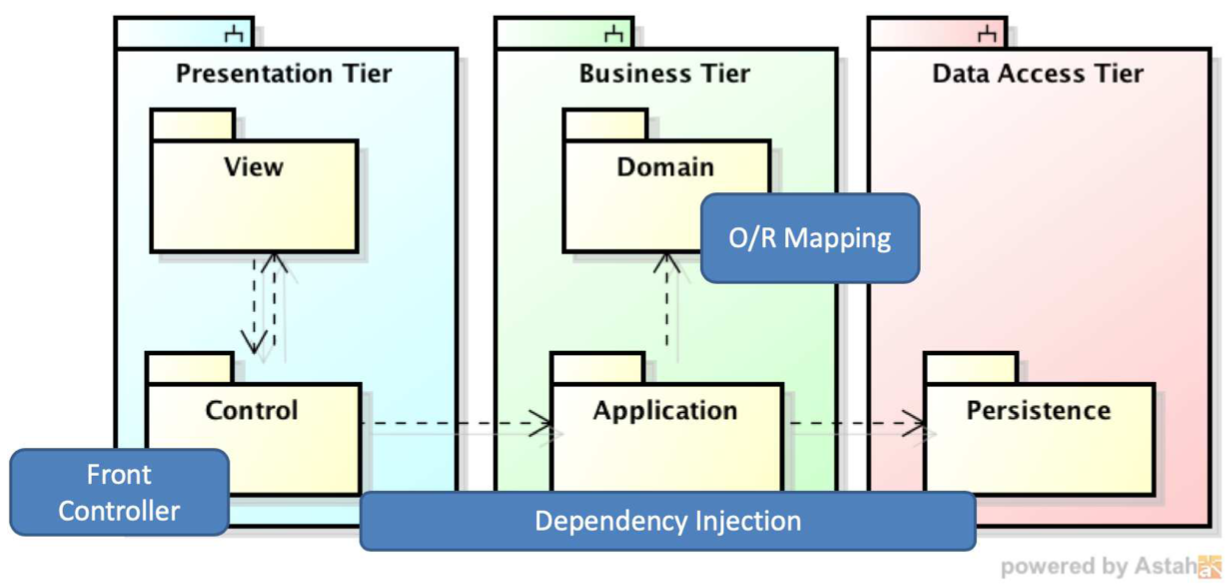
\includegraphics[width=.9\textwidth]{figuras/fig-arquitetura-frameweb.png} 
    \caption{Arquitetura sugerida pelo método FrameWeb~\cite{souza:2020}.}
    \label{fig-arquitetura-frameweb}
\end{figure}


\begin{itemize}
    \item \textbf{Lógica de Apresentação}: tem o objetivo de prover a interface gráfica
        ao usuário e é dividida em dois pacotes. O primeiro é o pacote \textbf{Visão},
        que contém as páginas \textit{Web}, folhas de estilo, imagens, scripts que executam do lado do cliente,
        e outros arquivos relacionados exclusivamente com a exibição de informações ao usuário.
        O segundo é o pacote \textbf{Controle}, que envolve classes de ação que lidam com as requisições
        feitas pelos componentes do pacote \textbf{Visão}, utilizando a infraestrutura do \textit{framework} 
        Controlador Frontal e chamando serviços oferecidos pelo pacote \textbf{Aplicação};

    \item \textbf{Lógica de Negócio}: tem o objetivo de prover os serviços do sistema e é dividida
        em dois pacotes. O primeiro é o pacote \textbf{Aplicação}, que implementa os casos de uso 
        definidos na especificação de requisitos. O segundo é o pacote \textbf{Domínio}, que contém 
        as classes de domínio do sistema, que representam conceitos do domínio do problema;

    \item \textbf{Lógica de Acesso a Dados}: tem o objetivo de prover a persistência dos dados e 
        possui um único pacote, chamado \textbf{Persistência}. Esse pacote é responsável pelo armazenamento
        dos objetos em mídias de longa duração, como bancos de dados. O FrameWeb propõe ainda o uso de um
        \textit{framework} ORM (\textit{Object-Relational Mapping}) com o padrão DAO (\textit{Data Access Object})~\cite{alur:2003}
        para adicionar uma camada de abstração a mais na manipulação de objetos no banco de dados relacional.
\end{itemize}

Além das arquiteturas lógicas e físicas do sistema, é também na fase de Projeto de Sistema
que são modelados os artefatos que serão implementados na próxima etapa. O FrameWeb define
quatro modelos baseados no diagrama de classes UML~\cite{souza:2007,souza:2020}:


\begin{itemize}
    \item \textbf{Modelo de Entidade}: diagrama de classes UML representando o domínio do 
        problema e o mapeamento dos objetos que serão persistidos. Esse modelo tem um forte
        papel para a implementação da Camada de Domínio;

    \item \textbf{Modelo de Persistência}: diagrama de classes UML que representa as classes
        DAO. Para cada uma das classes de domínio que será persistida, é criada uma classe DAO
        que define os métodos de persistência para uma dada classe, guiando assim a 
        construção da Camada de Persistência;
    
    \item \textbf{Modelo de Navegação}: diagrama de classes UML que representa as páginas \textit{Web}
        e outros elementos da Camada de Apresentação. Esse modelo auxilia o desenvolvedor a
        implementar os pacotes Visão e Controle uma vez que todos os atributos e fluxos de 
        navegação baseados nos estímulos enviados pelo usuário são definidos nele;

    \item \textbf{Modelo de Aplicação}: diagrama de classes UML que representa as classes
        responsáveis pela implementação dos casos de uso, além das dependências dos pacotes
        Controle, Domínio e Persistência.
\end{itemize}

A proposta inicial do método FrameWeb foi feita pensando em \textit{frameworks} MVC \cite{souza:2007},
no entanto, com a popularidade dos \textit{frameworks} SPA, o método foi adaptado para suportar
esse tipo de \textit{framework}, que se diferencia do primeiro principalmente pelo fato de possuir elementos que se comportam tanto como \textit{controller} quanto como 
\textit{view} e por focar na interação destes~\cite{hoppe:2023}.


%%%%%%%%% Início de seção. %%%%%%%%%
\section{Frameworks}
\label{sec-fundteo-framework}

\citeonline{schmidt:2004} definem \textit{frameworks} como um conjunto de artefatos de software, sejam eles
classes, objetos ou componentes, que colaboram entre si para prover uma arquitetura reutilizável
para aplicações de uma certa família. Dessa forma, os \textit{frameworks} visam o reuso de soluções, o que
pode reduzir o tempo de desenvolvimento e deixar a manutenção do software mais fácil~\cite{gamma:2000}.

\textit{Frameworks} podem ser classificados de diversas formas, como \textit{frameworks} MVC,
\textit{frameworks} SPA, \textit{frameworks} ORM, entre outros. Nesta seção, serão abordados
com detalhes os \textit{frameworks} ORM e SPA, e por fim, o \textit{framework} utilizado neste trabalho,
que se encaixa nesta categoria.

\subsection{Frameworks SPA}
\label{sec-fundteo-framework-spa}

\textit{Frameworks} SPA (\textit{Single Page Application} ou Aplicações de Página Única) são \textit{frameworks} que implementam
aplicações \textit{Web} executadas por uma única página, ou seja, a página é carregada apenas uma vez 
ao iniciar a aplicação~\cite{emmitt:2015}. Toda a responsabilidade de renderizar a aplicação é
transferida ao \textit{browser} do cliente, o chamado \textit{Client-Side Rendering} (CSR), ou Renderização do Lado do Cliente,
e então o DOM (\textit{Document Object Model} ou Modelo de Documento por Objetos) é manipulado via \textit{JavaScript} para alterar a visualização da 
página~\cite{emmitt:2015,konshin:2018}. Isso faz com que, ao interagir com as páginas, não 
seja necessário carregar a página inteira novamente, apenas os dados e componentes que foram alterados, 
tornando a experiência de usuário mais fluida ao navegar pelo sistema. 

Devido a essa característica, os \textit{frameworks} SPA se tornaram muito populares em aplicações
Web, dentre os mais utilizados estão o Angular\footnote{Angular, \url{https://angular.io}}
e o Vue,\footnote{Vue, \url{https://vuejs.org}} além do React,\footnote{React, \url{https://react.dev}}
que, apesar de ser uma biblioteca, também implementa aplicações SPA.

No entanto, este tipo de aplicação possui também problemas, sendo eles o alto tempo de carregamento
inicial, pois é necessário carregar todo o código da aplicação de uma vez, e a dificuldade de
indexação por mecanismos de busca (SEO), uma vez que estes tendem a classificar melhor
páginas que carregam mais rápido~\cite{konshin:2018}. Isso é uma grande desvantagem para um sistema
de vendas, por exemplo, que precisa ser indexado por mecanismos de busca para que o site seja mais
fácilmente encontrado por possíveis consumidores.

\subsection{Frameworks ORM}
\label{sec-fundteo-framework-orm}

Grande parte dos sistemas precisam que seus dados sejam armazenados de alguma forma e,
dentre os diversos tipos de sistemas de armazenamento, os bancos de dados relacionais são
os mais utilizados. Esses sistemas possuem uma estrutura de dados organizada em tabelas, e a partir de 
um sistema de gerenciamento de banco de dados relacional (SGBDR), é possível manipular esses dados
por meio da linguagem SQL (\textit{Structured Query Language} ou Linguagem Estruturada de Consulta)~\cite{silberschatz:2019}.

Por outro lado, muitas aplicações utilizam linguagens de programação orientadas a objetos (OO), o que
pode tornar a manipulação de dados em um banco de dados relacional mais complexa, uma vez que
as SGBDR representam os dados como tabelas, enquanto as linguagens OO os representam como um grafo 
de objetos interconectados. Essa é a chamada incompatibilidade de paradigmas (\textit{paradigm mismatch})~\cite{hibernate:2010,bauer:2005}.

Na década de 80, surgiram os \textit{frameworks} ORM (Mapeamento Objeto/Relacional), que têm como objetivo
mapear os objetos da aplicação para as tabelas do banco de dados relacional. O uso desses \textit{frameworks} 
facilita a manipulação de dados para o desenvolvedor, que precisa apenas informar ao \textit{framework}
como transformar objetos e seus atributos em tabelas e colunas e chamar métodos simples, sem precisar
aprender uma nova linguagem como SQL.

Alguns exemplos de \textit{frameworks} ORM são o Hibernate para Java,\footnote{Hibernate, \url{https://hibernate.org}}
Entity Framework para .NET,\footnote{Entity Framework, \url{https://docs.microsoft.com/pt-br/ef}} e o 
Prisma para TypeScript.\footnote{Prisma, \url{https://www.prisma.io}}



\subsection{Next.js}
\label{sec-fundteo-framework-next}

\patricia{Acho que aqui vc precisa incluir qual é o modelo de execução do Next. Vc diz que não é MVC, certo? 
Mas o que é? Como as coisas funcionam? Explique com algum exemplo, como o fluxo funciona…
Uma outra coisa importante é: vc usou o next fullstack… o que isso quer dizer em termos da tecnologia 
que é feita para frontend? Explique isso melhor…}

O Next.js é um \textit{framework Web} construído em cima do React, biblioteca JavaScript \textit{front-end open-source}
baseada em componentes, voltada para a construção da interface de usuário e mantida pela Meta.\footnote{Meta, \url{https://about.meta.com}}
Por ser uma biblioteca, o React não implementa 
técnicas de roteamento, o que faz com que exista a dependência do uso de outras bibliotecas, 
como o React Router.\footnote{React Router, \url{https://reactrouter.com}}
Já o Next.js faz isso de forma nativa. 

Outro ponto de destaque são as técnicas de renderização, 
além do CSR, o Next.js implementa os métodos \textit{Server-Side Rendering} (SSR), ou Renderização do Lado do Servidor,
e \textit{Static Site Generation} (SSG), ou Geração Estática de Site, que permitem que o código da aplicação seja executado
no servidor, e resolvem os problemas de SEO e tempo de carregamento inicial, comuns de 
aplicações SPA. Um detalhe que tem feito com que esse \textit{framework}
ganhe popularidade, é o fato de que o desenvolvedor pode escolher qual método de renderização
utilizar para cada página do sistema~\cite{vercel:2023}.

Outro ponto alto do Next.js é a facilidade de se fazer o \textit{deploy} da aplicação, que pode ser feito
de forma otimizada com o provedor de \textit{hosting} da Vercel,\footnote{Vercel, \url{https://vercel.com}} 
plataforma que desenvolveu o \textit{framework}~\cite{nextjs:2023}.

\textit{JavaScript} é uma linguagem leve e interpretada, que é utilizada para adicionar interatividade e dinamicidade
à páginas \textit{Web}. No entanto, por ser uma linguagem de tipagem fraca e dinâmica, ela pode ser propensa a erros
em tempo de execução, o que, em sistemas de porte elevado, pode se tornar um grande problema~\cite{typescript:2024}.
Nesse ambiente, surge o \textit{TypeScript}, linguagem de programação de alto nível desenvolvida e mantida pela Microsoft.\footnote{Microsoft, \url{https://www.microsoft.com}}
O \textit{TypeScript} é convertido em código \textit{JavaScript}, e portanto fornece todas as características desta, além de adicionar suporte a tipos, 
permitindo a detecção de erros em tempo de compilação,
e outras funcionalidades, como interfaces, \textit{generics} e \textit{unions}~\cite{typescript:2024}.

O Next.js suporta o uso de \textit{TypeScript} em suas aplicações, o que pode ser uma grande vantagem para
desenvolvedores que desejam ter um código mais seguro e menos propenso a erros.

% \vitor{Esta seção está muito pequena. Se você está falando de TypeScript por ela ser a linguagem usada no desenvolvimento com Next.js, então você pode incluir essa informação e mais este parágrafo na seção do Next.js.}

% ==============================================================================
% PG - Sophie Dilhon
% Capítulo 3 - Especificação de Requisitos
% ==============================================================================
\chapter{Especificação de Requisitos}
\label{chap-especificacao-requisitos}

Este capítulo tem como objetivo apresentar a especificação de requisitos do SCAP (Sistema de Controle de Afastamento de Professores), 
assim como os modelos de casos de uso e de classes levantados por \citeonline{duarte:2014} e \citeonline{prado:2015}, que serão utilizados como base para a implementação do sistema.

\section{Descrição do Escopo}
\label{sec-espec-escopo}
O SCAP é um sistema que visa auxiliar o gerenciamento das solicitações de
afastamento de professores do Departamento de Informática (DI) da Universidade Federal do Espírito Santo (UFES)
para participação em eventos, sejam eles no Brasil ou no exterior. 
Nesses casos, o professor deve submeter uma solicitação de afastamento temporário
que será avaliada pelos professores do DI, e em alguns casos,
pelo Conselho do Centro Tecnológico (CT) e Pró-Reitoria de Pesquisa e Pós-Graduação (PRPPG) da UFES.
Ao ser aprovada em todas as instâncias, o afastamento temporário é autorizado.

Para eventos no Brasil, as solicitações tramitam apenas no DI, e devem ser
aprovadas pela Câmara Departamental (formada pelos funcionários do Departamento
e representantes discentes). Dessa forma, o professor envia seu pedido para a
lista de e-mails dos funcionários do DI, endereçado ao Chefe de Departamento,
cargo exercido temporariamente por um professor do DI. Caso nenhum membro
da Câmara Departamental se oponha ao pedido em até dez dias, o afastamento é autorizado.

Para eventos no exterior, um professor, que não tenha parentesco com o solicitante,
é escolhido para ser o relator do pedido. Após emitido o parecer do relator, o
processo deve ser aprovado pela Câmara Departamental, como no caso de eventos no Brasil.
Além disso, a solicitação deve ser aprovada pelo Conselho Departamental do CT e pela PRPPG.
Depois de ser aprovado por todos os envolvidos, o afastamento é autorizado
e o pedido é publicado no Diário Oficial da União. 
No entanto, o SCAP é responsável por assistir o processo apenas dentro do DI,
não havendo uma integração com os processos no CT e na PRPPG.

O objetivo do SCAP é agilizar e simplificar o processo para os professores
e secretários do DI, automatizando o envio de e-mails aos membros envolvidos
e utilizando formulários para a criação dos documentos necessários.


\section{Modelos de Casos de Uso}
\label{sec-espec-casos-uso}

Na Tabela~\ref{tab:atores} são apresentados os atores do SCAP, identificados
por \citeonline{duarte:2014} no levantamento de requisitos do sistema.

\begin{table}[h!]
    \centering
    \caption{Atores do Sistema}
    \label{tab:atores}
    \begin{tabular}{|p{5cm}|p{10cm}|}
    \hline
    \textbf{Atores} & \textbf{Descrição}\\ \hline
    Professor & Professor efetivo do DI \\ \hline
    Secretário & Secretário do DI \\ \hline
    Chefe de Departamento & Professor do DI que está realizando a função administrativa de chefe ou subchefe do departamento  \\ \hline
    \end{tabular}
\end{table}

O secretário é responsável pela administração do sistema. Sendo assim,
ele deve cadastrar os professores, e seus parentescos, além dos mandatos
de chefes e subchefes do departamento. Outras tarefas incluem, cadastrar
as decisões do CT e PRPPG (em casos de eventos no exterior), e arquivar
processos que forem concluídos.

O professor pode cadastrar solicitações de afastamento e também se manifestar
contra pedidos de outros professores, caso esteja dentro do prazo para tal.
Se for adicionado como relator de um pedido de afastamento no exterior,
o professor deve emitir um parecer sobre o mesmo, e assim decidir se o
DI aprova ou não tal solicitação.

O chefe de departamento é um professor que foi eleito para exercer a função
administrativa durante um período de tempo. Assim, além das funcionalidades
comuns a um professor, ele também é responsável por nomear relatores
para pedidos de afastamento no exterior.


O SCAP foi dividido em dois módulos: Cadastral e Núcleo. O primeiro é responsável pela parte
cadastral, ou seja, casos de uso dos secretários. Já o segundo, abrange
as funcionalidades de professores e chefes de departamento. Uma versão mais
completa e detalhada pode ser vista em~\cite{duarte:2014,prado:2015}.
As Figuras~\ref{fig:casos-de-uso-cadastral} e~\ref{fig:casos-de-uso-nucleo} apresentam
os diagramas de casos de uso do SCAP.

\begin{figure}
    \centering
    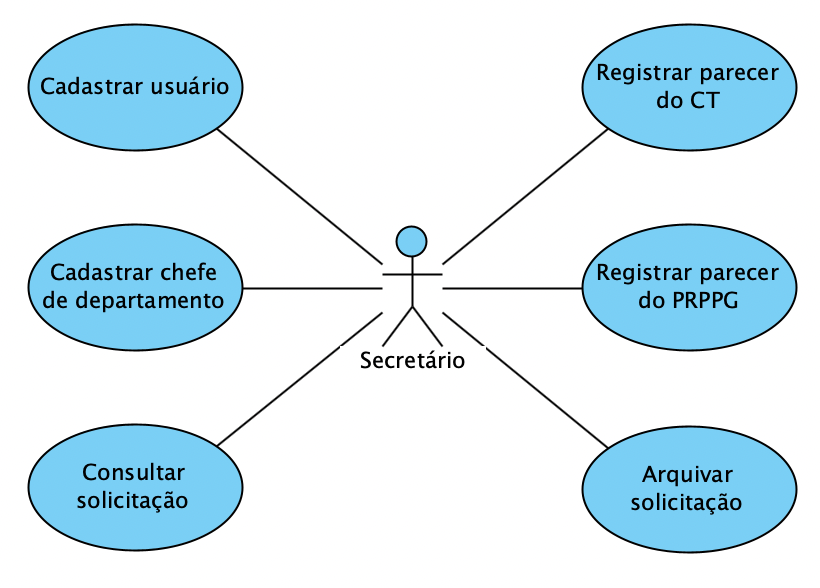
\includegraphics[width=0.6\textwidth]{figuras/fig-caso-cadastral.png}
    \caption{Diagrama de Casos de Uso do subsistema Cadastral~\cite{prado:2015}.}
    \label{fig:casos-de-uso-cadastral}
\end{figure}

Em \textbf{Cadastrar Usuário}, o secretário cadastra um novo usuário no sistema, sendo
este um professor ou um secretário, junto de seus dados. Já em \textbf{Cadastrar chefe de departamento},
o secretário cadastra o mandato do chefe ou subchefe do departamento, assim como suas datas de início e fim.

Os casos de uso \textbf{Registrar parecer do PRPPG} e \textbf{Registrar parecer do CT}, ocorrem
apenas em casos de afastamento no exterior. O secretário é responsável por registrar as decisões
da PRPPG e do CT, respectivamente, quando estes aprovam ou não um pedido de afastamento.

Em \textbf{Arquivar solicitação}, o secretário arquiva um processo que foi concluído, ou seja, que
já passou por todas as instâncias e foi aprovado. \textbf{Consultar Solicitação} é um caso de uso
comum aos professores e secretários, e permite que o usuário consulte o andamento e os dados de um
pedido de afastamento.


\begin{figure}
    \centering
    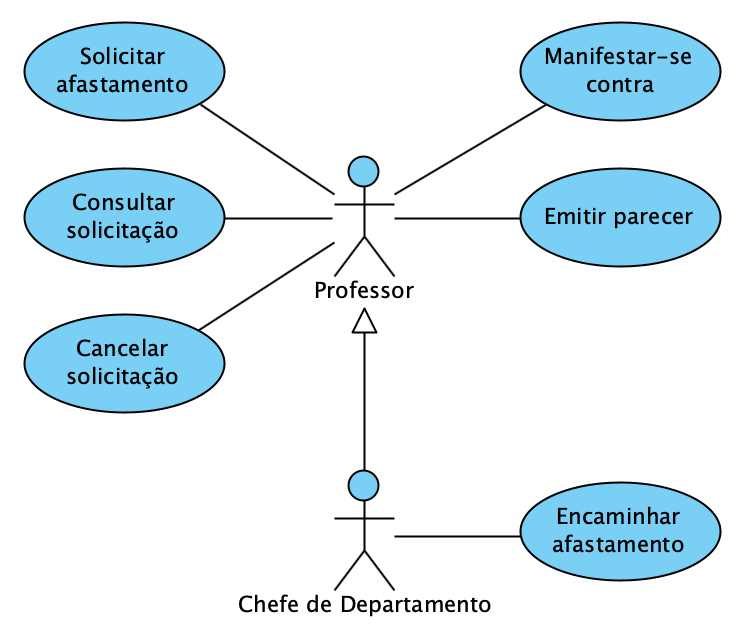
\includegraphics[width=0.6\textwidth]{figuras/fig-caso-nucleo.png}
    \caption{Diagrama de Casos de Uso do subsistema Núcleo~\cite{prado:2015}.}
    \label{fig:casos-de-uso-nucleo}
\end{figure}


O caso de uso \textbf{Solicitar afastamento} é o principal caso de uso do sistema, e permite
que um professor solicite um afastamento para participar de um evento. Para isso devem ser informadas
as datas de início e fim, o nome do evento e se este é nacional ou internacional. 
Enquanto em \textbf{Cancelar solicitação}, o professor pode cancelar um pedido feito por ele próprio,
alterando assim o estado do processo para cancelado.

O professor pode ainda \textbf{Manifestar-se contra} um pedido de afastamento de 
outro professor, caso esteja dentro do prazo para tal, registrando o motivo de sua opinião.
Uma reunião deve então ser agendada para que os professores decidam se o afastamento será aprovado ou não.
Por último, \textbf{Emitir parecer} é um caso de uso exclusivo de professores que foram nomeados
como relator de um pedido de afastamento no exterior. O professor deve cadastrar um parecer sobre a solicitação.

O chefe de departamento, além das funcionalidades comuns a um professor, também pode \textbf{Encaminhar afastamento},
ou seja, indicar um professor como relator para um pedido de afastamento no exterior. 


\section{Análise do SCAP}
\label{sec-espec-analise-scap}

A Figura~\ref{fig:diagrama-classes} apresenta o diagrama de classes do SCAP, adaptado
do levantamento feito por~\citeonline{prado:2015}, juntamente com o que havia sido
levantado anteriormente por~\citeonline{duarte:2014}.

\vitor{A figura foi tirada de \cite{prado:2015}? Se sim, incluir \cite{prado:2015} ao final da legenda (\textit{label}) da figura. Está estranha a relação entre a classe \textsf{Parentesco} e a associação que a clases \textsf{Professor} tem com si própria. Se você refez o diagrama de classes do \citeonline{prado:2015}, precisamos corrigir essa relação.}
\sophie{A figura foi refeita a partir do diagrama de classes de \cite{prado:2015}, só alterando as cores e a propriedade é chefe em Mandato, o resto esta como foi apresentado por ele. Mas concordo que a relação entre Professor e Parentesco está estranha.}
\vitor{Precisa corrigi-la.}

\begin{figure}
    \centering  
    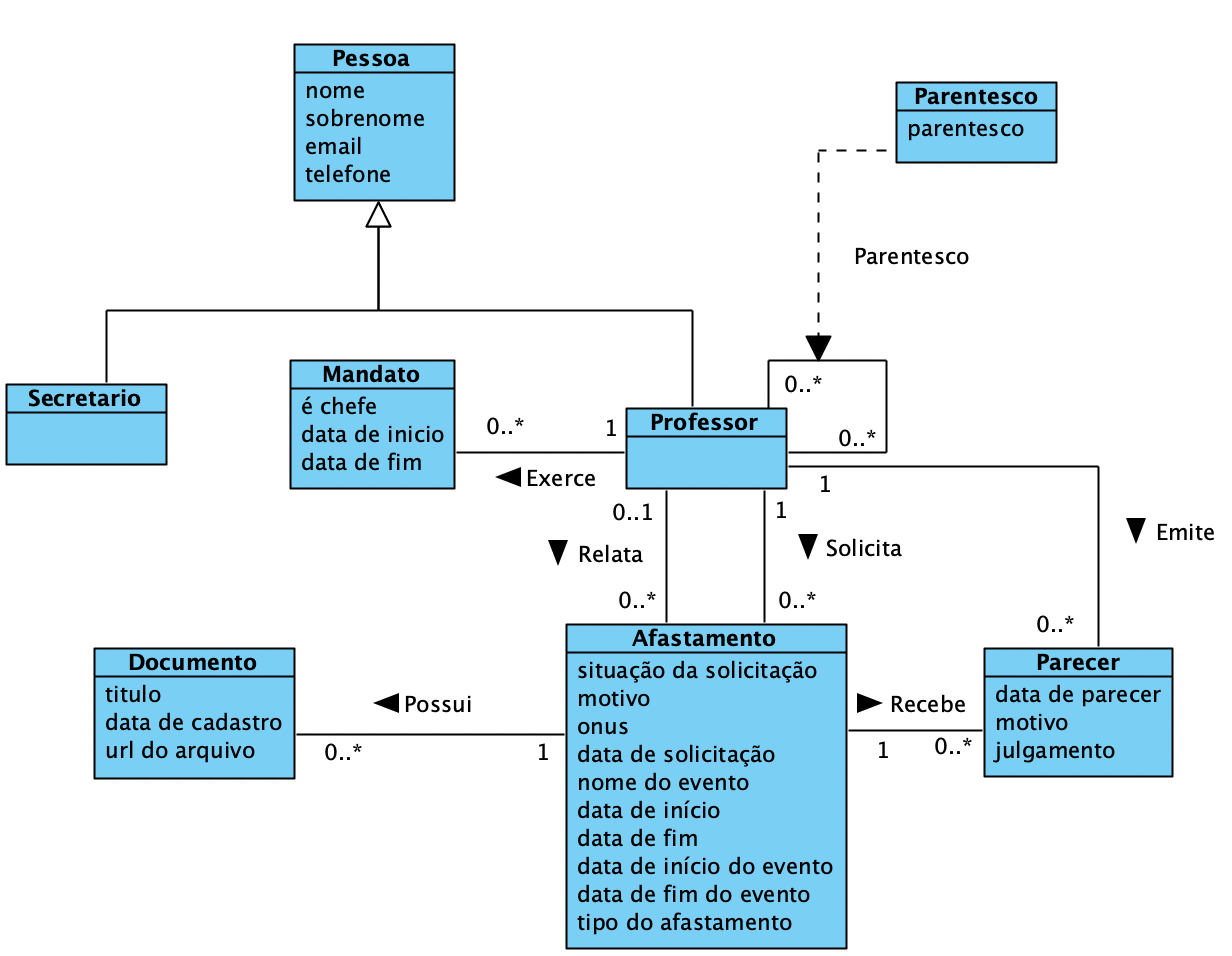
\includegraphics[width=0.9\textwidth]{figuras/fig-diagrama-classes.png}
    \caption{Diagrama de Classes do SCAP, adaptado de~\cite{prado:2015}.}
    \label{fig:diagrama-classes}
\end{figure}

As classes \textbf{Professor} e \textbf{Secretario}, que representam os professores
e secretários do DI, respectivamente, herdam as propriedades da classe \textbf{Pessoa},
que contém as informações pessoais do usuário. A classe \textbf{Parentesco} 
guarda relações de parentesco que podem existir entre professores do DI.
A classe \textbf{Mandato} representa o tempo do mandato, de chefe ou subchefe do departamento,
que o professor está exercendo.

A classe \textbf{Afastamento} guarda informações sobre os pedidos de afastamento
feitos pelos professores, como as datas de início e fim, o nome do evento e etc.
Este pode ou não possuir um \textbf{Documento} associado, e deve possuir um \textbf{Relator}
caso seja um pedido de afastamento no exterior. Um professor pode ser relator de vários afastamentos,
mas seu \textbf{Parecer} é único para cada solicitação de afastamento internacional.


Restrições de integridade complementam o modelos de classes, que por muitas vezes não são
capazes de representá-las por notações gráficas. Abaixo estão listadas as restrições
levantadas por~\citeonline{duarte:2014} e posteriormente ampliadas por~\citeonline{prado:2015}:

\begin{itemize}
    \item Um professor não pode ser nomeado como relator, nem emitir um parecer, para sua própria solicitação de afastamento;
    \item Um professor não pode ser relator de um afastamento solicitado por um parente;
    \item A data de início de um afastamento não pode ser posterior a data de fim do mesmo afastamento;
    \item A data de início de um mandato de professor não pode ser posterior a data de fim do mesmo mandato;
    \item Não pode haver mais de dois professores (chefe e subchefe de departamento) exercendo um mandato ao mesmo tempo;
    \item O secretário do departamento não pode abrir uma solicitação de afastamento.
\end{itemize}
% ==============================================================================
% PG - Sophie Dilhon
% Capítulo 4 - Projeto Arquitetural e Implementação
% ==============================================================================
\chapter{Projeto Arquitetural e Implementação}
\label{chap-projeto}

Neste capítulo
são apresentados os passos de projeto arquitetural e desenvolvimento da aplicação.
Na Seção~\ref{sec-projeto-tecnologias} estão as tecnologias utilizadas, na Seção~\ref{sec-projeto-frameweb}
são exemplificados os modelos FrameWeb desenvolvidos para auxilio na implementação do SCAP.
A Seção~\ref{sec-projeto-arquitetura} mostra a arquitetura do sistema. 
Por fim, na Seção~\ref{sec-projeto-impl} são apresentadas capturas de tela da aplicação para
ilustrar o desenvolvimento do SCAP.

\vitor{A Seção~\ref{sec-projeto-arquitetura} não mostra a arquitetura, mas sim a estrutura do sistema pra implementação. A arquitetura teria que ser mostrada antes dos modelos FrameWeb, como é feito no documento de especificação de projeto.}


\section{Tecnologias Utilizadas}
\label{sec-projeto-tecnologias}

Neste projeto, utilizou-se a linguagem \textit{TypeScript} unida ao \textit{framework} Next.js.
A Tabela~\ref{tab-tecnologias} apresenta as tecnologias e bibliotecas utilizadas, suas funções e suas respectivas versões.
Dentre as tecnologias, destaca-se o MySQL, um sistema de gerenciamento de banco de dados relacional,
e o Prisma, um ORM (\textit{Object-Relational Mapping}) para Node.js, ferramenta utilizada
para mapear classes para tabelas, além de facilitar a manipulação de dados com o banco.

\begin{table}[h]
    \centering
    \caption{Tecnologias e Bibliotecas Utilizadas.}
    \label{tab-tecnologias}
    \begin{tabularx}{\textwidth}{|p{4cm}|X|p{2cm}|}%{|p{3cm}|p{5cm}|p{5cm}|}
        \hline
        \textbf{Tecnologia} & \textbf{Função} & \textbf{Versão} \\
        \hline
        TypeScript & Linguagem de programação & 5 \\
        \hline
        Next.js & \textit{Framework} para desenvolvimento \textit{Web} & 14.1.3 \\
        \hline
        Tailwind CSS & \textit{Framework} CSS para estilizar componentes & 3.3.0 \\
        \hline
        Axios & Cliente HTTP baseado em \textit{Promises} & 1.6.8 \\
        \hline
        Prisma & ORM (\textit{Object-Relational Mapping}) para Node.js & 5.11.0 \\
        \hline
        MySQL & Sistema de Gerenciamento de Banco de Dados Relacional & 8.3.0 \\
        \hline
        React Dropzone & Componente para \textit{upload} de arquivos & 14.2.3 \\
        \hline
        React Input Mask & Componente para máscaras de \textit{inputs} & 3.0.0 \\
        \hline
        React Toastify & Componente para notificações & 10.0.5 \\
        \hline
        Luxon & Biblioteca para manipulação de datas & 3.4.4 \\
        \hline
        uuid & Biblioteca para geração de identificadores únicos & 9.0.1 \\
        \hline
        NPM & Gerenciador de pacotes para \textit{Node.js} & 10.5.0 \\
        \hline
        Visual Paradigm & Ferramenta para modelagem de diagramas & 17.1 \\
        \hline
        \end{tabularx}
\end{table}




\section{Modelos FrameWeb}
\label{sec-projeto-frameweb}

Nessa seção são apresentados os modelos FrameWeb, construídos na fase de Projeto Arquitetural
do SCAP, com o objetivo de guiar a fase de implementação do sistema.

\subsection{Modelo de Entidades}
\label{subsec-frameweb-entidades}
O modelo de entidades de FrameWeb é um diagrama de classes UML que representam
os objetos de domínio do problema e seu mapeamento para a persistência no banco de dados
relacional. A partir dele são implementadas as classes da camada de domínio~\cite{souza:2007}.

A Figura~\ref{fig-modelo-entidades} apresenta o modelo de entidades do SCAP. O modelo foi feito
a partir do diagrama de classes mostrado anteriormente, com adaptações para a plataforma 
escolhida para a implementação do sistema, dessa forma são apresentados os tipos
de cada propriedade. A Figura~\ref{fig-modelo-entidades-enum} apresenta
os tipos enumerados do modelo de entidades do SCAP.

\begin{figure}
    \centering
    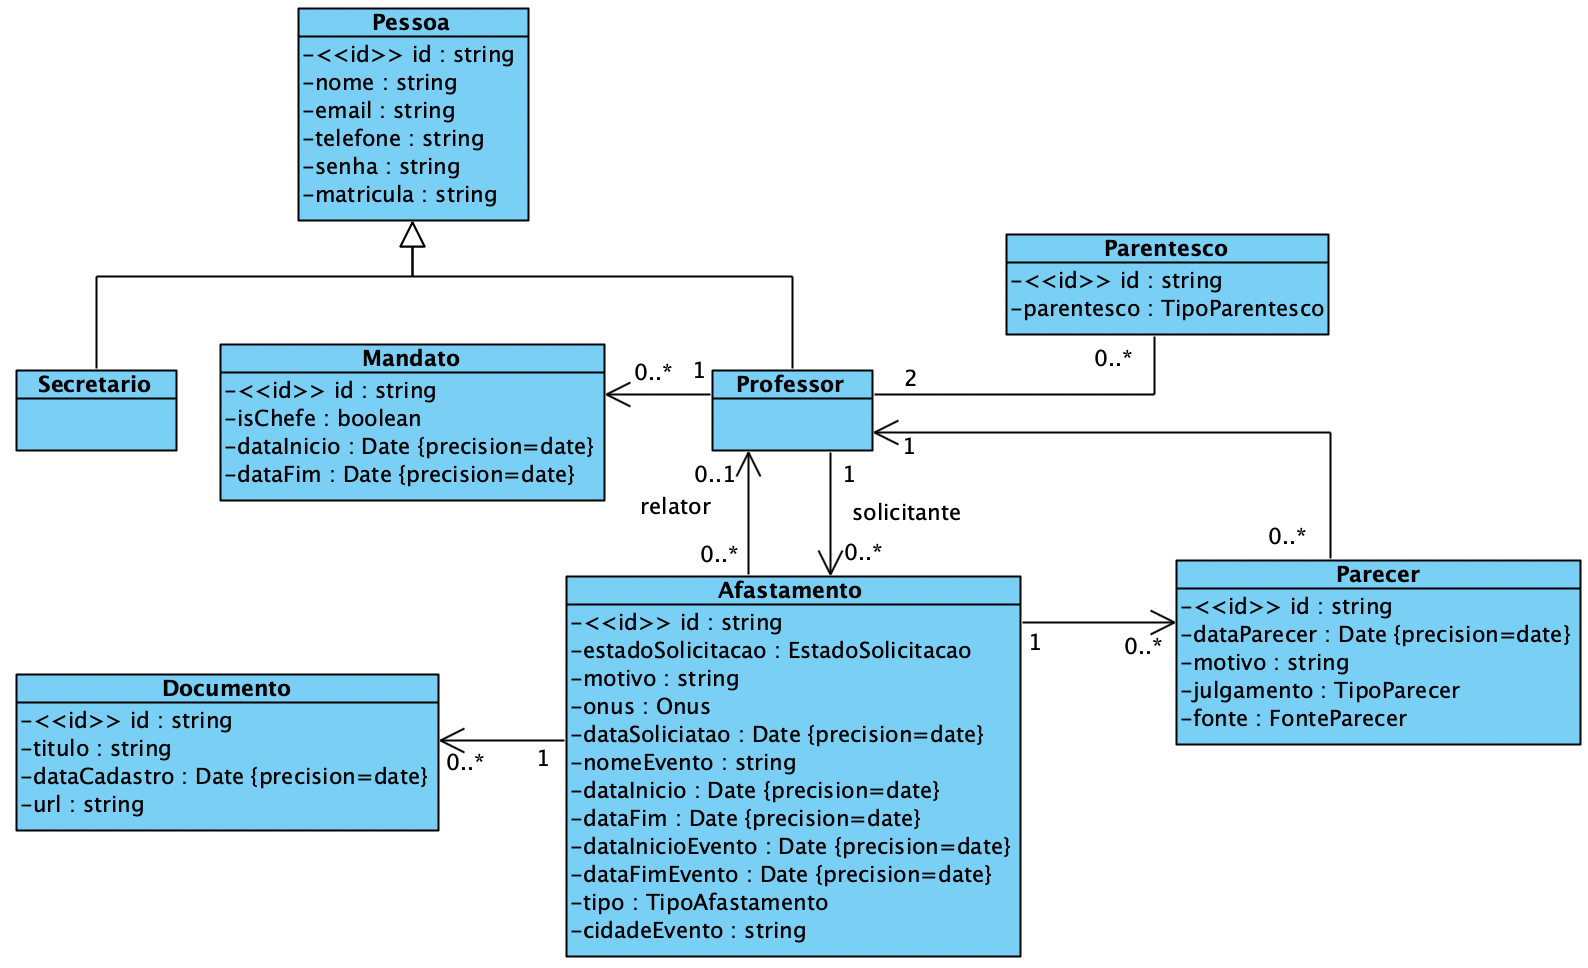
\includegraphics[width=1\textwidth]{figuras/fig-modelo-entidades.png}
    \caption{Modelo de Entidades do SCAP.}
    \label{fig-modelo-entidades}
\end{figure}

\begin{figure}
    \centering
    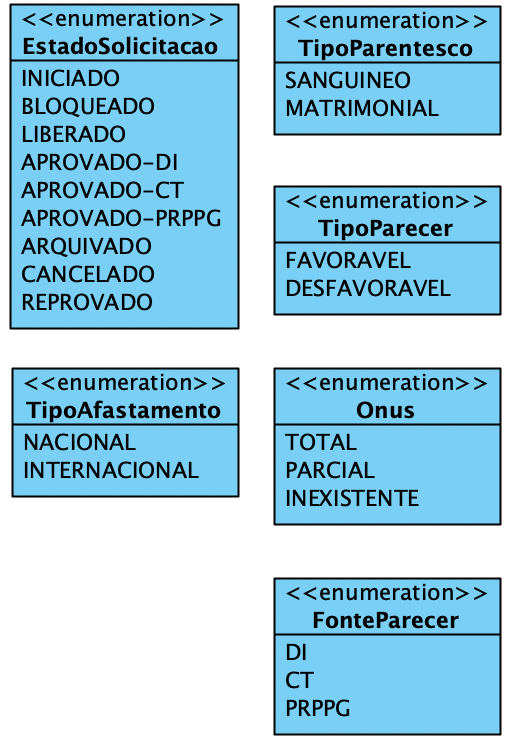
\includegraphics[width=0.5\textwidth]{figuras/fig-modelo-entidades-enum.png}
    \caption{Tipos Enumerados do Modelo de Entidades do SCAP.}
    \label{fig-modelo-entidades-enum}
\end{figure}


Os diagramas~\ref{fig-diagrama-estado-nacional} e~\ref{fig-diagrama-estado-internacional} apresentam os fluxos de estados
para solicitações de afastamento do tipo nacional e internacional, respectivamente.
Explicitando os estados que uma solicitação de afastamento pode assumir e as transições entre eles,
de acordo com determinadas ações. Um exemplo de fluxo para um afastamento nacional é descrito abaixo:

\begin{enumerate}
    \item O professor solicita um afastamento nacional, este é criado no estado \textbf{INICIADO};
    \item Um professor do DI manifesta-se contra a solicitação, o afastamento passa para o estado \textbf{BLOQUEADO};
    \item Após votação favorável do colegiado, o secretário registra a aprovação do afastamento que muda para o estado \textbf{APROVADO\_DI};
    \item Por fim, o secretário arquiva a solicitação, modificando seu estado para \textbf{ARQUIVADO}.

\end{enumerate}

\begin{figure}[h!]
    \centering
    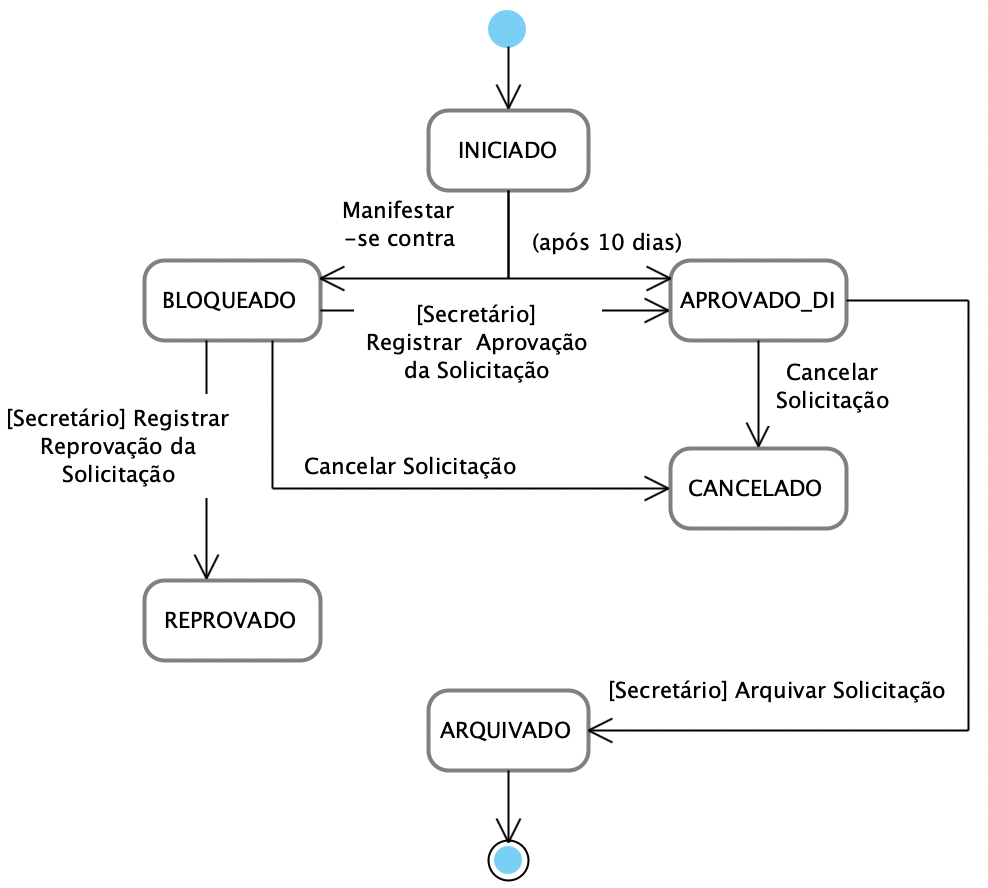
\includegraphics[width=0.8\textwidth]{figuras/fig-diagrama-estado-nacional.png}
    \caption{Diagrama de Estados da Solicitação de Afastamento Nacional do SCAP.}
    \label{fig-diagrama-estado-nacional}
\end{figure}


\begin{figure}[h!]
    \centering
    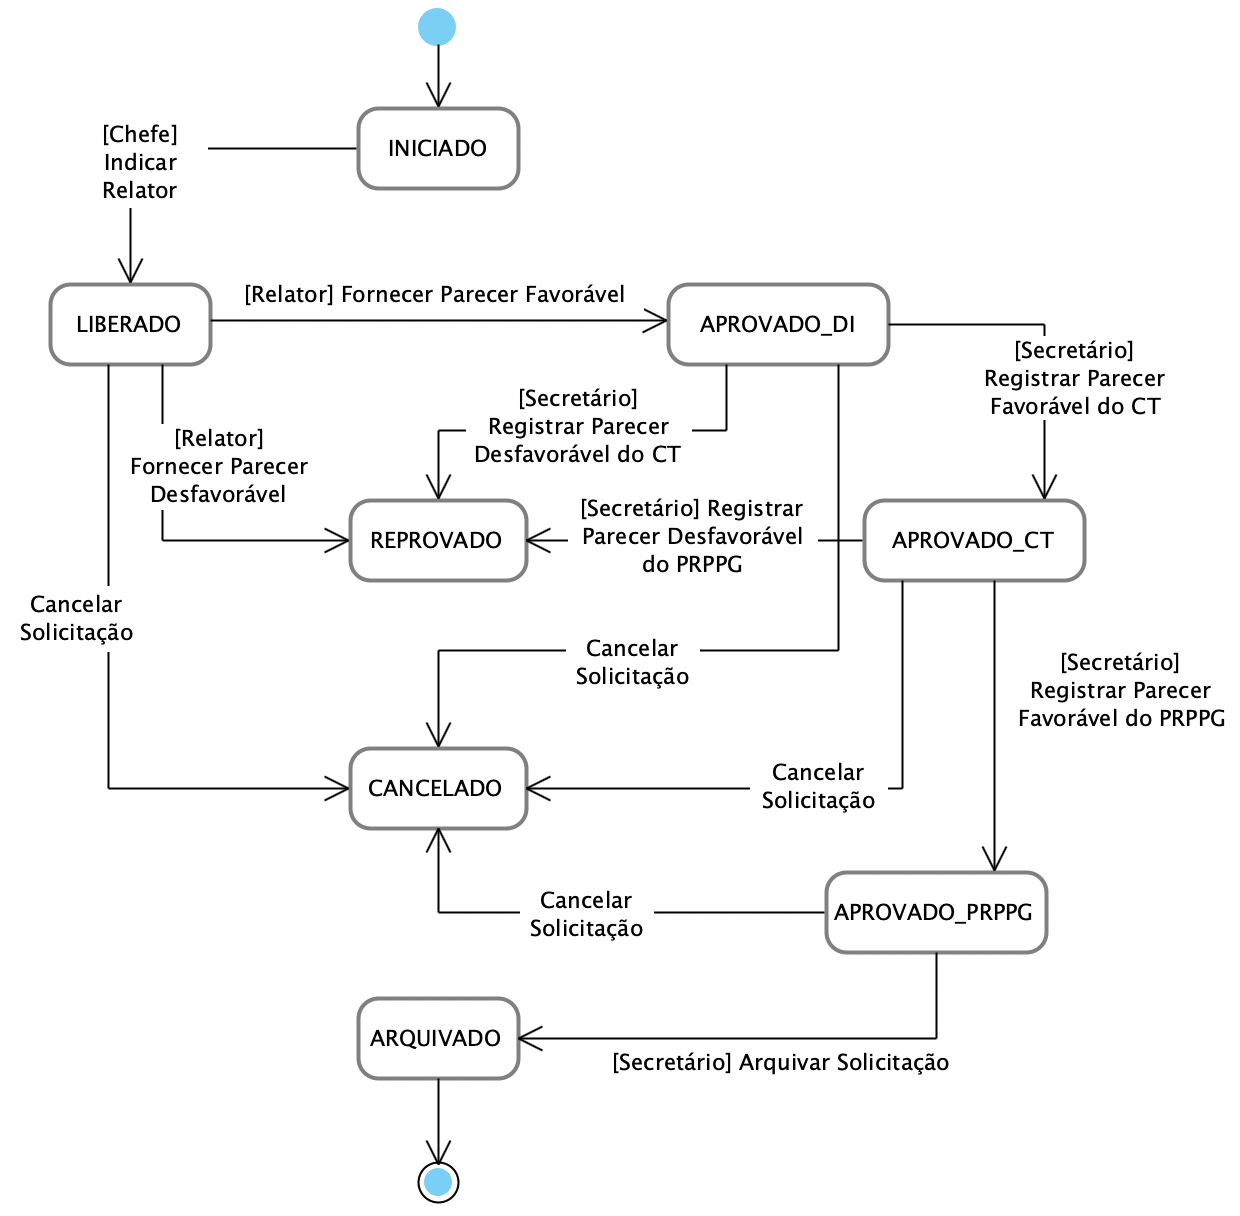
\includegraphics[width=0.9\textwidth]{figuras/fig-diagrama-estado-internacional.png}
    \caption{Diagrama de Estados da Solicitação de Afastamento Internacional do SCAP.}
    \label{fig-diagrama-estado-internacional}
\end{figure}


\subsection{Modelo de Persistência}
\label{subsec-frameweb-persistencia}

O modelo de persistência de FrameWeb é um diagrama de classes UML que representa
as classes responsáveis pela persistência das classes de domínio no banco de dados~\cite{souza:2007}.
Foi utilizado o padrão \textit{Repository} para a implementação das classes de persistência,
este propõe uma camada de separação entre o domínio e o mapeamento de dados.


Para isso, foi criada uma interface base (\textbf{IBaseRepositoy}) que define os métodos comuns a todas as classes de persistência,
sendo eles: \textit{get} para buscar todos os elementos com base nos filtros passados como parâmetro,
\textit{post} para criar um novo elemento, \textit{getById} para buscar um elemento a partir de seu
\textit{id} e \textit{delete}. A Figura~\ref{fig-modelo-persist-base} apresenta essa interface e a
classe \textit{Repository} que a implementa. O tipo genérico \textit{T} representa a classe de domínio
sendo manipulada, ou seja, em \textbf{AfastamentoRepository} o método \textit{getById}
retorna um elemento da classe \textbf{Afastamento}.


\begin{figure}[h!]
    \centering
    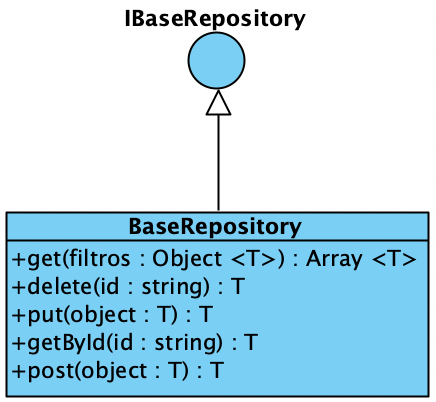
\includegraphics[width=0.4\textwidth]{figuras/fig-modelo-persist-base.png}
    \caption{Interface e Implementação do Repository Base.}
    \label{fig-modelo-persist-base}
\end{figure}


As interfaces do modelo herdam \textbf{IBaseRepositoy}, enquanto as classes \textit{Repository} estendem a
classe \textbf{BaseRepository}. De modo que todas as classes de persistência possuam, além dos métodos
específicos dessas, os métodos comuns definidos na interface base. As Figuras~\ref{fig-modelo-persist}
apresentam o modelo de persistência do SCAP.

\begin{figure}[h!]
    \centering
    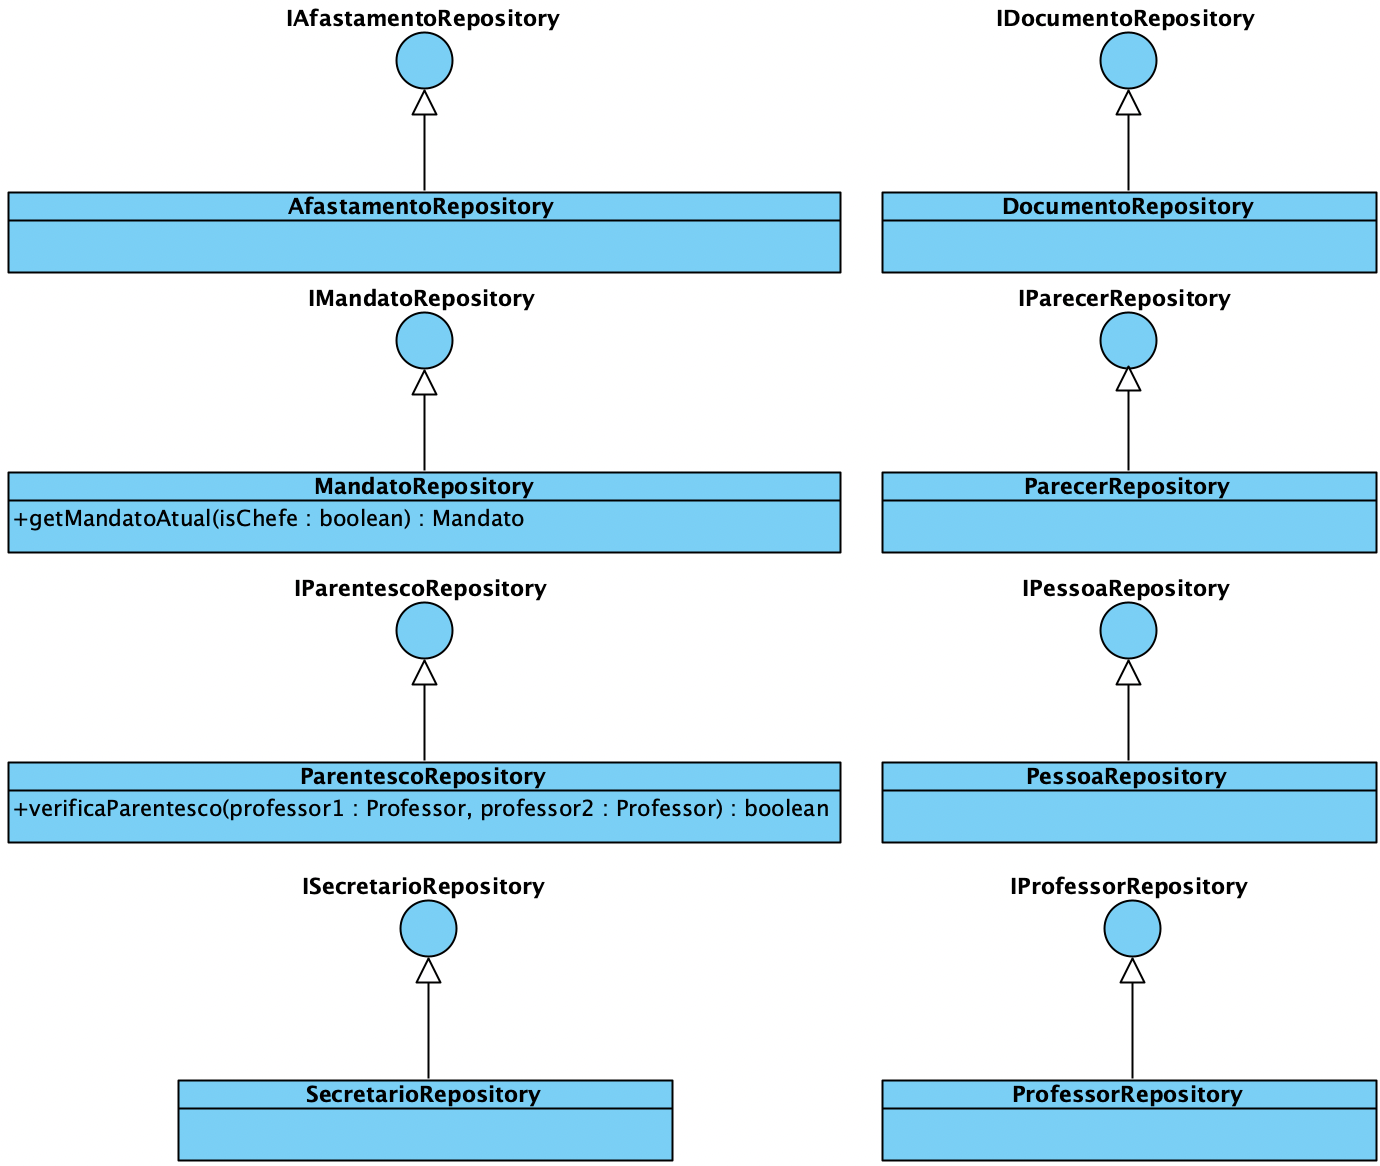
\includegraphics[width=0.9\textwidth]{figuras/fig-modelo-persist.png}
    \caption{Modelo de Persistência do SCAP.}
    \label{fig-modelo-persist}
\end{figure}



\subsection{Modelo de Navegação}
\label{subsec-frameweb-navegacao}

O Modelo de Navegação é um diagrama de classe da UML que representa os diferentes componentes que
formam a camada de Lógica de Apresentação, como páginas Web, formulários HTML e classes de ação do \textit{framework} específico~\cite{souza:2007}. 
Esse modelo é utilizado para guiar a implementação dos pacotes Visão e Controle.

A Tabela~\ref{tab-estereotipos-navegacao} apresenta os estereótipos UML utilizados no modelo de navegação do SCAP,
propostos por~\citeonline{hoppe:2023} como uma adaptação, para \textit{frameworks} SPA,
dos estereótipos propostos originalmente por~\citeonline{souza:2007}.

\begin{table}[h!]
    \centering
    \caption{Estereótipos UML para Modelos de Navegação~\cite{hoppe:2023}.}
    \label{tab-estereotipos-navegacao}
    \begin{tabular}{|p{3cm}|p{12cm}|}
        \hline
        \textbf{Estereótipo} & \textbf{Descrição} \\
        \hline
        (Nenhum)    & Controladora de um framework Front Controller ou a parte controladora de um component de um framework SPA. \\
        \hline
        <<Page>>    & Página Web estática ou dinâmica. \\
        \hline
        <<Partial>> & Parte de uma página HTML que é gerada em tempo de execução por meio de AJAX. \\
        \hline
        <<Form>>    & Formulário HTML \\
        \hline
    \end{tabular}
\end{table}

A Figura~\ref{fig-modelo-navegacao-afast} apresenta o modelo de navegação do SCAP para os casos de uso
\textbf{Cancelar Afastamento}, \textbf{Cadastrar Afastamento} e \textbf{Consultar Afastamento}.

\begin{figure}
    \centering
    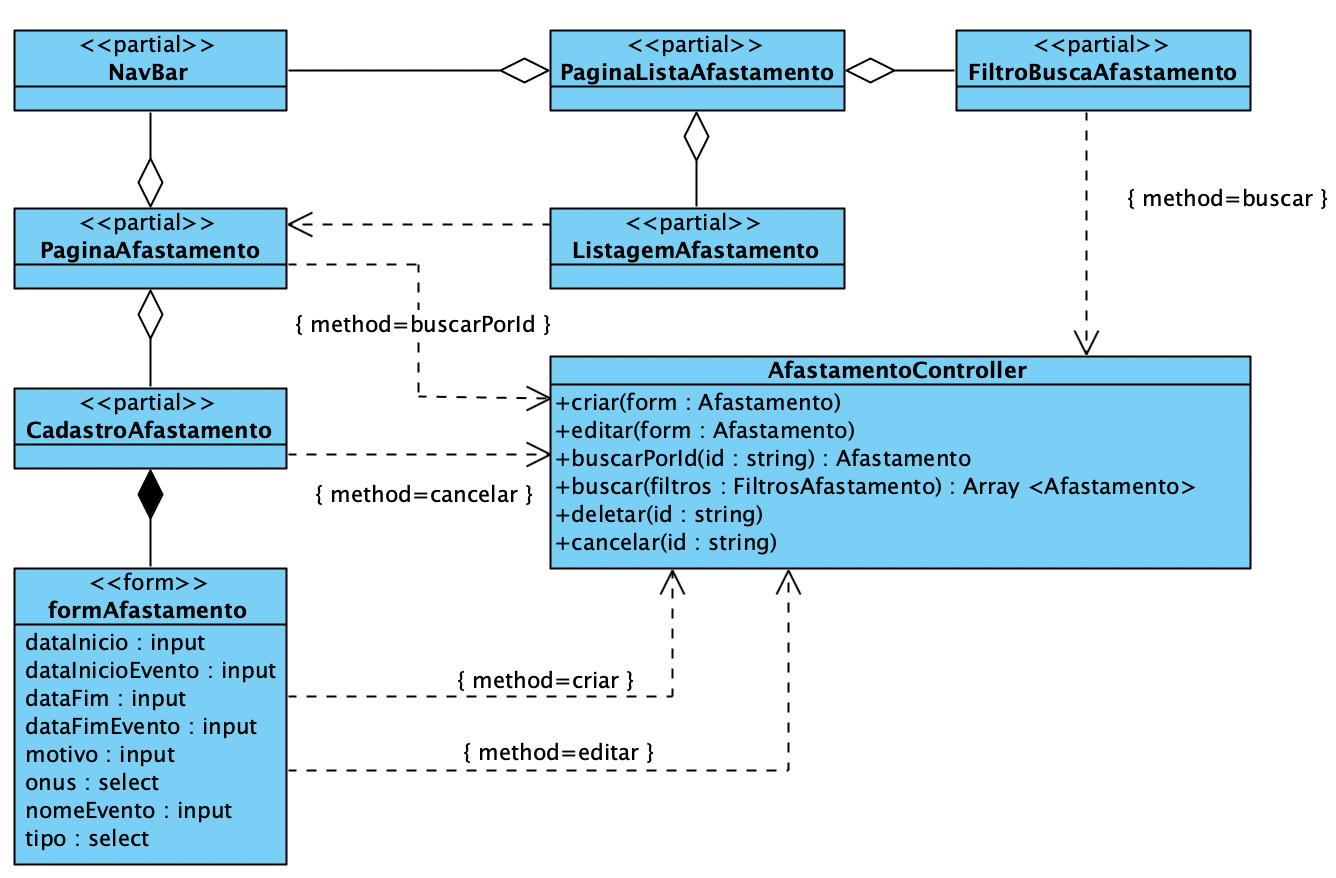
\includegraphics[width=1\textwidth]{figuras/fig-modelo-naveg-afast.png}
    \caption{Modelo de Navegação do SCAP.}
    \label{fig-modelo-navegacao-afast}
\end{figure}

A \textbf{PaginaListaAfastamento} é responsável por listar os afastamentos cadastrados.
Ela possui um componente filtro (\textbf{FiltroBuscaAfastamento}), em que é possível buscar
os afastamentos por diferentes critérios, definidos pela interface mostrada na Figura~\ref{fig-interface-filtro-afast}.
O componente \textbf{ListagemAfastamento} consiste de uma tabela que lista os afastamentos buscados,
cada linha da tabela possui um botão que redireciona para a página de detalhes do afastamento (\textbf{PaginaAfastamento}).

\begin{figure}
    \centering
    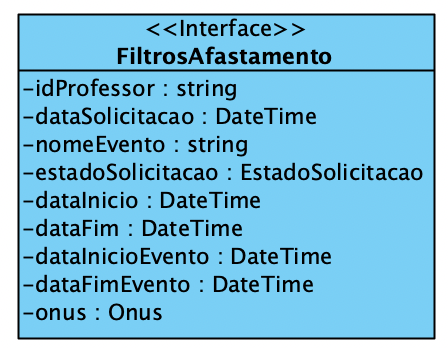
\includegraphics[width=0.4\textwidth]{figuras/fig-interface-filtro-afast.png}
    \caption{Interface Filtro Afastamento.}
    \label{fig-interface-filtro-afast}
\end{figure}

Se redirecionado para a \textbf{PaginaAfastamento} a partir do componente \textbf{ListagemAfastamento},
o \textit{partial} possui o atributo \textbf{id} inicializado com o \textit{id} do afastamento, e é
utilizado para fazer uma chamada ao método \textbf{buscarPorId} da \textit{controller} \textbf{AfastamentoController}.
Caso o usuário seja o solicitante do afastamento, ele pode cancelá-lo clicando em um botão que faz uma chamada ao método
\textbf{cancelar} da \textit{controller} \textbf{AfastamentoController}.

Quando não possui um \textit{id} inicializado, o \textit{partial} é utilizado para criar um novo afastamento,
o usuário deve então preencher os campos do formulário e clicar em um botão que faz uma chamada ao método
\textbf{criar} da \textit{controller} \textbf{AfastamentoController}.


\begin{figure}
    \centering
    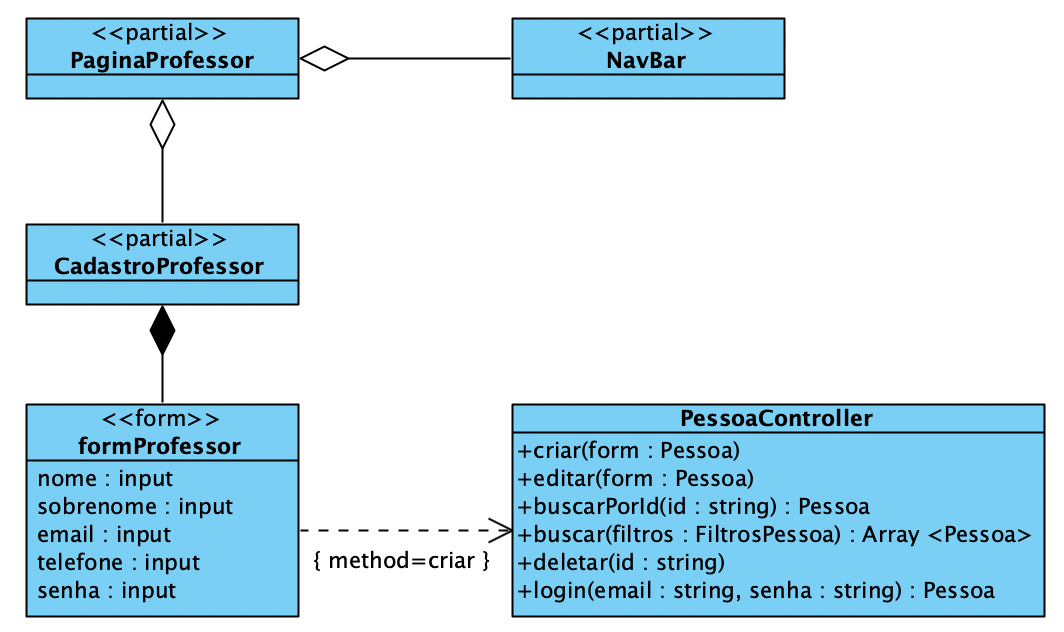
\includegraphics[width=0.9\textwidth]{figuras/fig-modelo-naveg-cadast.png}
    \caption{Modelo de Navegação do SCAP do Caso de Uso Cadastrar Professor.}
    \label{fig-modelo-navegacao-professor}
\end{figure}

A Figura~\ref{fig-modelo-navegacao-professor} apresenta o modelo de navegação do SCAP para o caso de uso
\textbf{Cadastrar Professor}. Na \textbf{PaginaProfessor} o secretário pode cadastrar um novo professor,
para isso ele deve preencher os campos do formulário e clicar em um botão que faz uma chamada ao método
\textbf{criar} da \textit{controller} \textbf{PessoaController}.

O componente \textbf{NavBar} presente em ambos os modelos de navegação é responsável por exibir
no topo da tela uma barra de navegação com links para as páginas principais do sistema, como a página inicial,
a página de listagem de afastamentos e a página de cadastro de professores. Ele é um componente
comum a todas as páginas do sistema, exceto à tela de \textit{login}.

\subsection{Modelo de Aplicação}
\label{subsec-frameweb-aplicacao}
O Modelo de Aplicação é um diagrama de classes da UML que representa as classes de
serviço, que são responsáveis pela codificação dos casos de uso, e suas dependências~\cite{souza:2007}.
Por ele pode-se visualizar a dependência entre os pacotes Controle (classes de ação),
Aplicação (classes de serviço) e Persistência (interfaces \textit{Repository}). 

As figuras~\ref{fig-modelo-aplicacao-1} e~\ref{fig-modelo-aplicacao-2} contém os Modelos de Aplicação.
As solicitações dos usuários são tratadas pelas classes de controle, que por sua vez
chamam as classes de serviço para realizar as operações de negócio, que por fim acessam
as classes de persistência para realizar as operações de leitura e escrita no banco de dados.


\begin{figure}[h!]
    \centering
    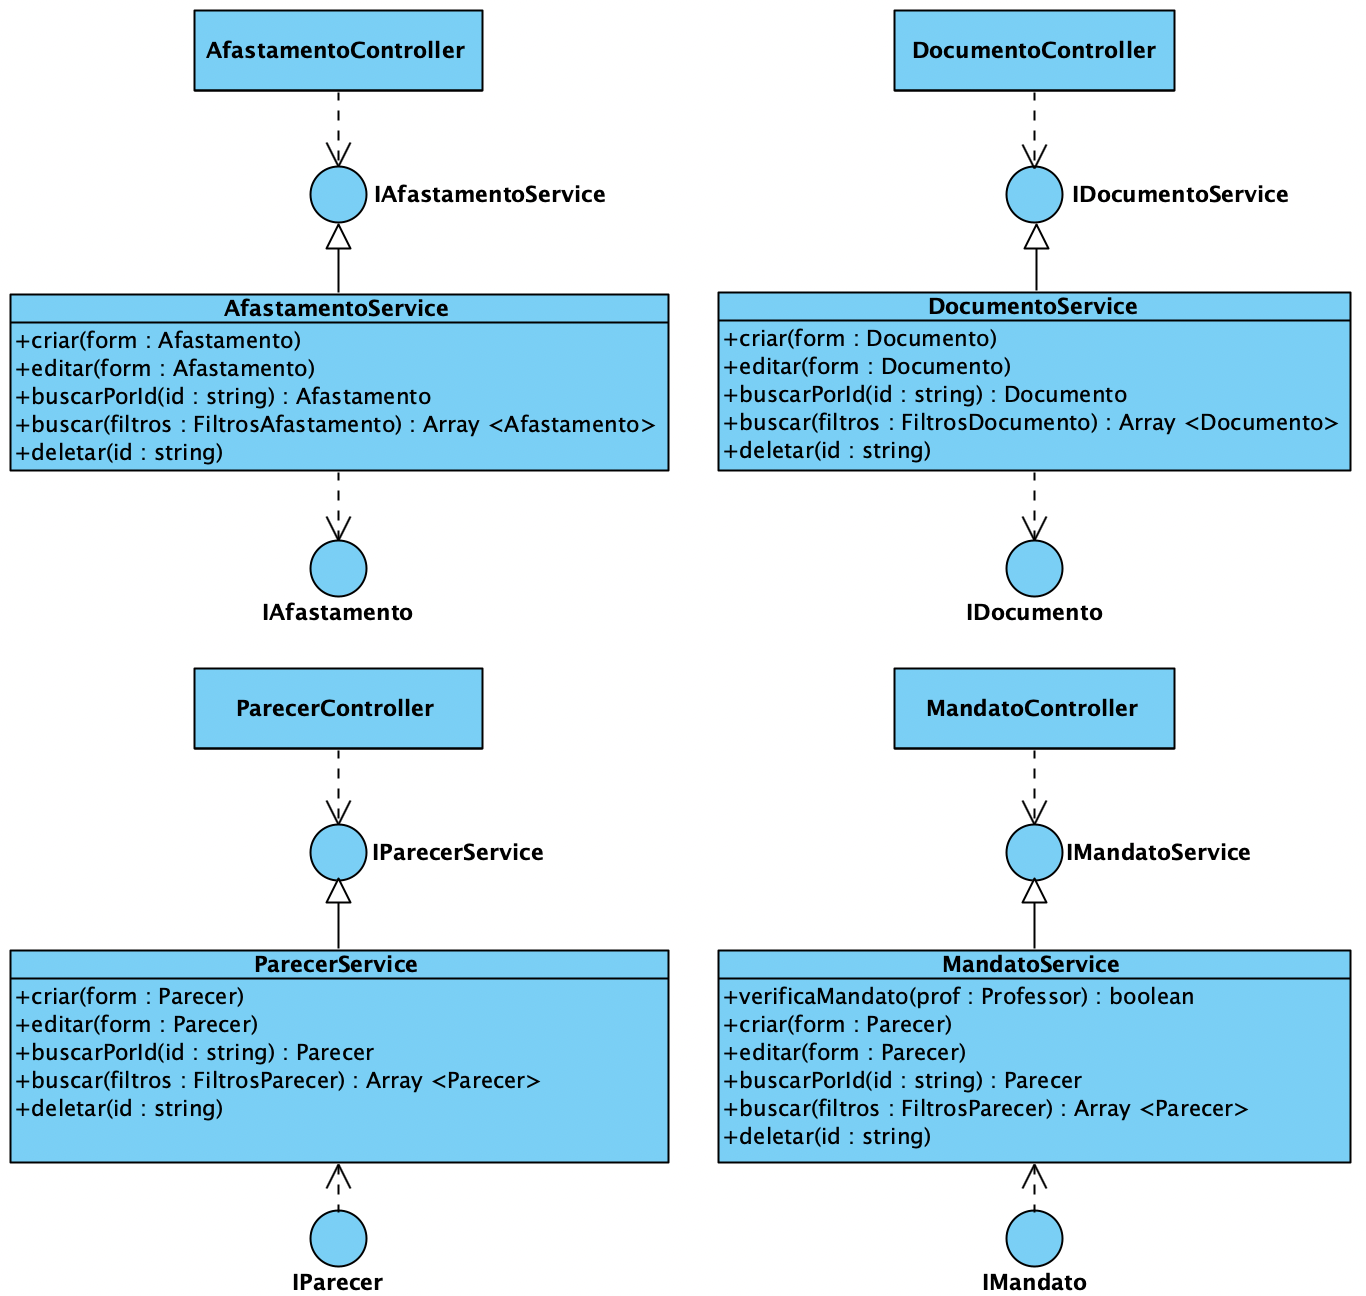
\includegraphics[width=0.9\textwidth]{figuras/fig-modelo-apl-1.png}
    \caption{Modelo de Aplicação do SCAP.}
    \label{fig-modelo-aplicacao-1}
\end{figure}


\begin{figure}[h!]
    \centering
    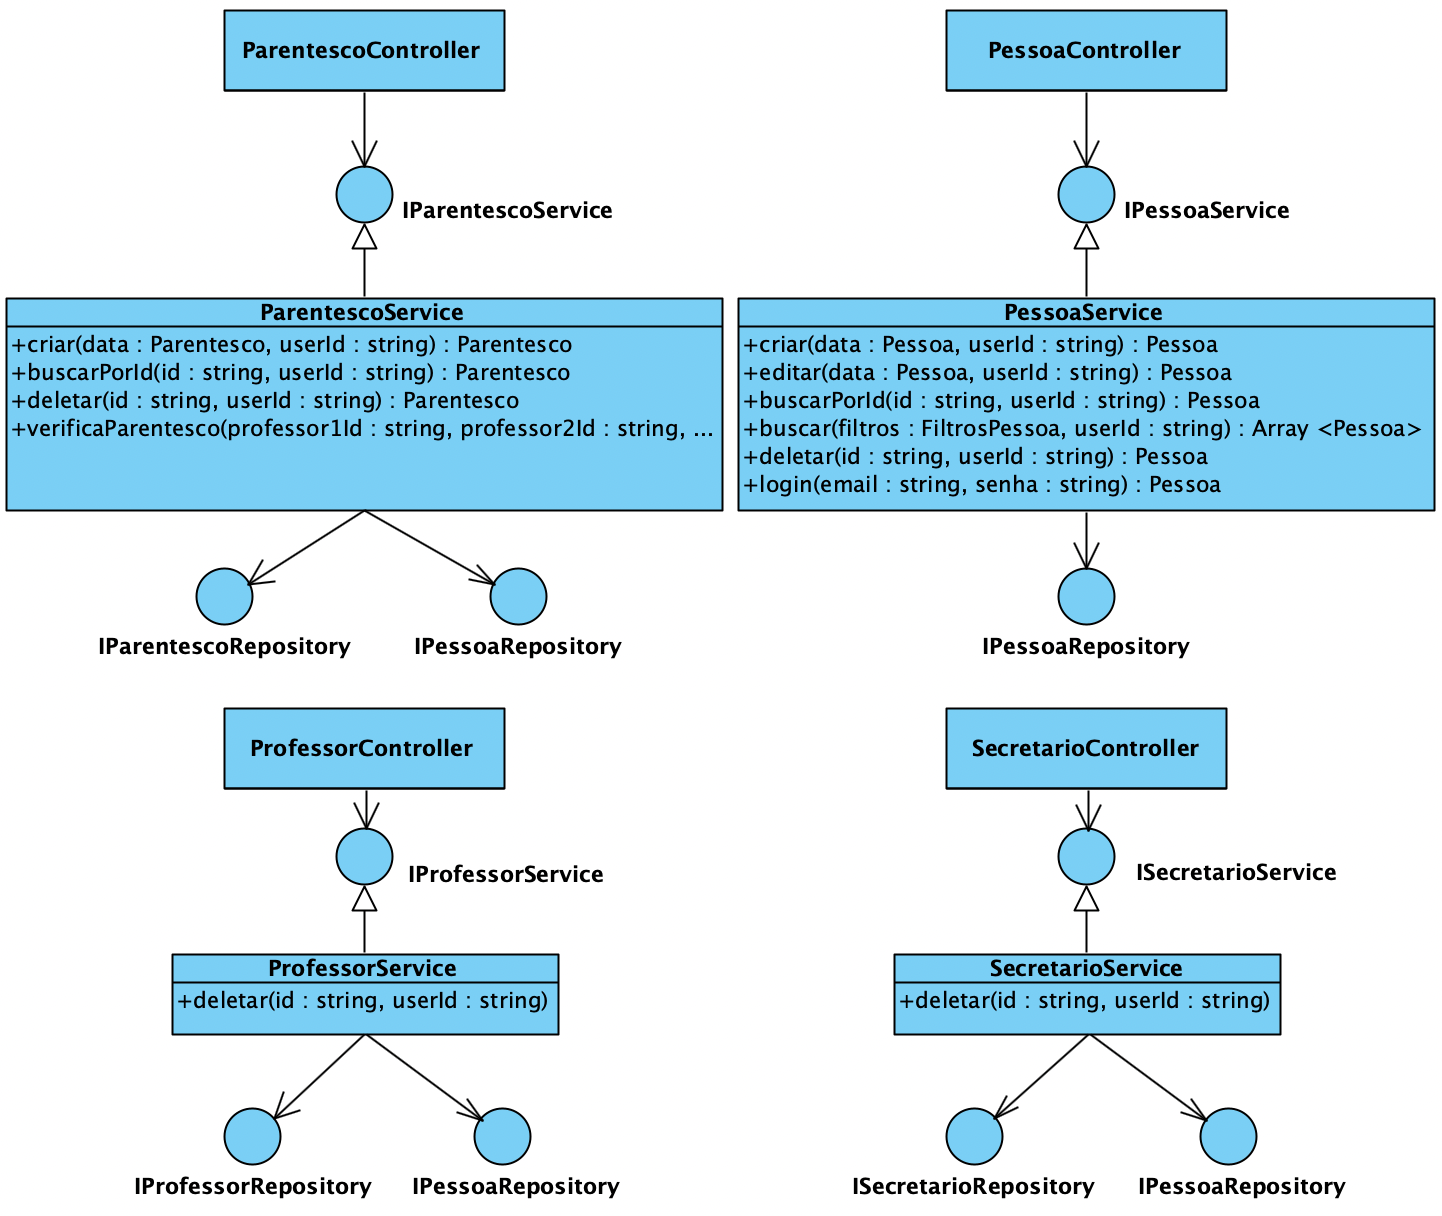
\includegraphics[width=0.9\textwidth]{figuras/fig-modelo-apl-2.png}
    \caption{Modelo de Aplicação do SCAP.}
    \label{fig-modelo-aplicacao-2}
\end{figure}



\section{Arquitetura do Sistema}
\label{sec-projeto-arquitetura}

Por ser um \textit{framework} de \textit{Single Page Application} (SPA), o Next.js funciona por meio de componentes,
e possui um padrão de \textit{design} diferente de projetos Java, por exemplo, que costumam utilizar
padrões como o \textit{Model-View-Controller} (MVC). 

A Figura~\ref{fig-pastas} apresenta a organização de pastas da implementação do SCAP. 
Na pasta \textbf{components} estão os componentes reutilizáveis, como o componente \textit{navbar} presente em todas as páginas do sistema.
A pasta \textbf{src} é a principal, nela estão contidas algumas pastas especiais controladas pelo \textit{framework}
como \textbf{pages} e \textbf{api}. A primeira, \textbf{pages}, transforma tudo que está dentro dela em uma rota do sistema,
ou seja, um arquivo \textit{index.js} em uma pasta chamada \textbf{pessoa} estará disponível como a rota \textit{/pessoa}.
De forma similar, a pasta \textbf{api} gera rotas de API a partir dos arquivos presentes nela.

Os arquivos presentes na pasta \textbf{api} possuem funções \textit{handler} especiais que são responsáveis por lidar com as requisições feitas ao servidor.
Estas funções utilizam as classes \textbf{controller} presente na pasta \textbf{lib} para manipular a requisição e retornar uma resposta.
Esta, por consequência, utiliza as classes \textbf{service} para realizar as operações de negócio, que por fim acessam as classes \textbf{reposity} para realizar
operações de leitura e escrita no banco de dados. As classes foram criadas seguindo o padrão de projeto \textit{Repository Pattern}.

No diretório \textbf{prisma} está presente o arquivo de configuração do Prisma, que contém o \textit{schema} do banco de dados e as \textit{migrations}
geradas pelo Prisma.

\vitor{Adicione uma frase explicando o que são as \textit{migrations}.}

\begin{figure}
    \centering
    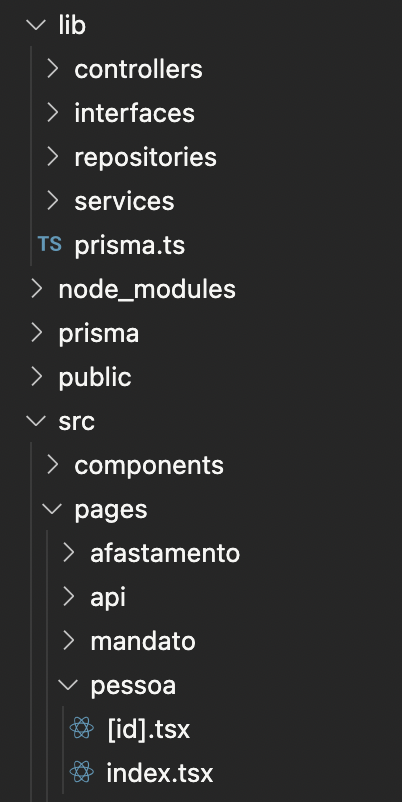
\includegraphics[width=0.4\textwidth]{figuras/fig-pastas.png}
    \caption{Arquitetura do SCAP.}
    \label{fig-pastas}
\end{figure}


\section{Implementação e Resultados}
\label{sec-projeto-impl}

Essa seção apresenta a implementação do SCAP, por meio de capturas de tela,
e discute os resultados obtidos.

\subsection{Login}
\label{subsec-projeto-login}

Para ter acesso ao SCAP, é necessário que o usuário realize o \textit{login} fornecendo o \textit{e-mail}
e senha cadastrados no sistema. A Figura~\ref{fig-login} apresenta a tela de \textit{login} do SCAP.
Por questões de segurança, sem o \textit{login} o usuário não consegue acessar as outras páginas do sistema
ou utilizar as rotas da API.

\begin{figure}[h!]
    \centering
    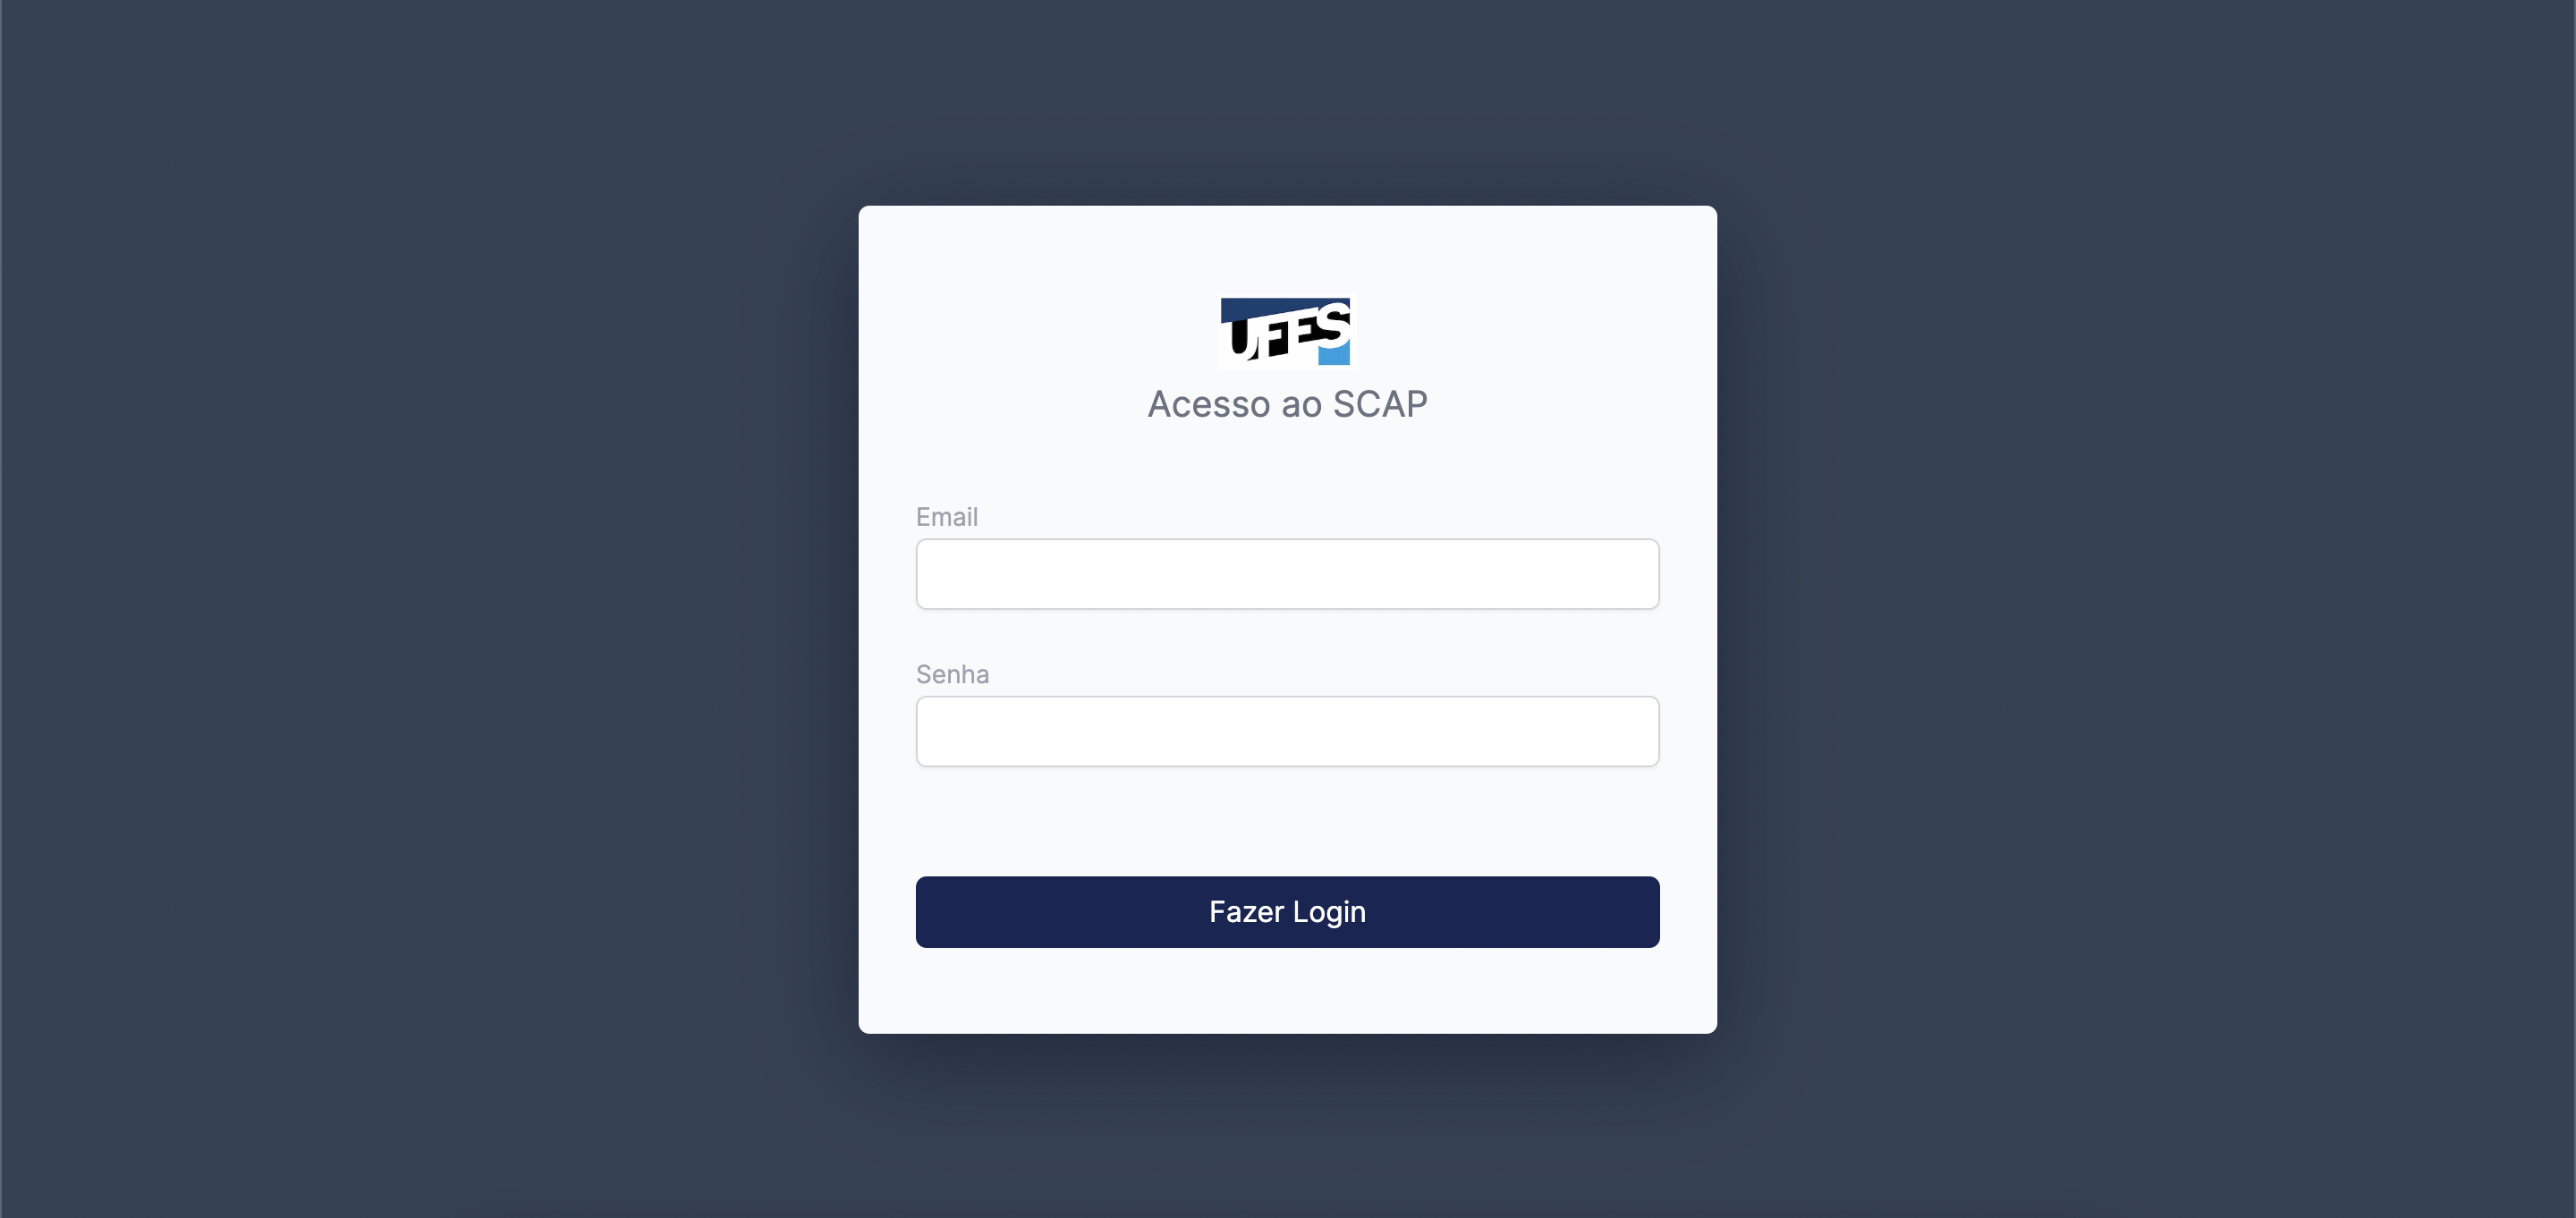
\includegraphics[width=\textwidth]{figuras/prints-app/fig-login.png}
    \caption{Tela de Login do SCAP.}
    \label{fig-login}
\end{figure}

Como mencionado anteriormente, existem dois tipos de usuários: secretário e professor. 
Os secretários são responsáveis por gerenciar os usuários e os estados dos afastamentos.
Já os professores podem solicitar afastamentos e visualizar o andamento das solicitações.
Dessa forma, as telas mudam de acordo com o tipo de usuário que está logado.


\subsection{Listagem de Afastamentos}
\label{subsec-projeto-afastamentos}

Ao completar o \textit{login}, o usuário é redirecionado para a página inicial do sistema, onde é possível
visualizar os afastamentos solicitados pelos professores. A Figura~\ref{fig-listagem-afastamentos} apresenta a tela de listagem de afastamentos
do SCAP. Nela é possível também buscar os afastamentos por diferentes critérios, como o nome do professor ou o estado do afastamento,
a Figura~\ref{fig-filtro-afastamentos} apresenta este filtro. Por fim, caso o usuário seja um professor,
o botão de solicitar afastamento estará disponível, ao clicá-lo o usuário é redirecionado para a página de cadastro de afastamento.

\begin{figure}[h!]
    \centering
    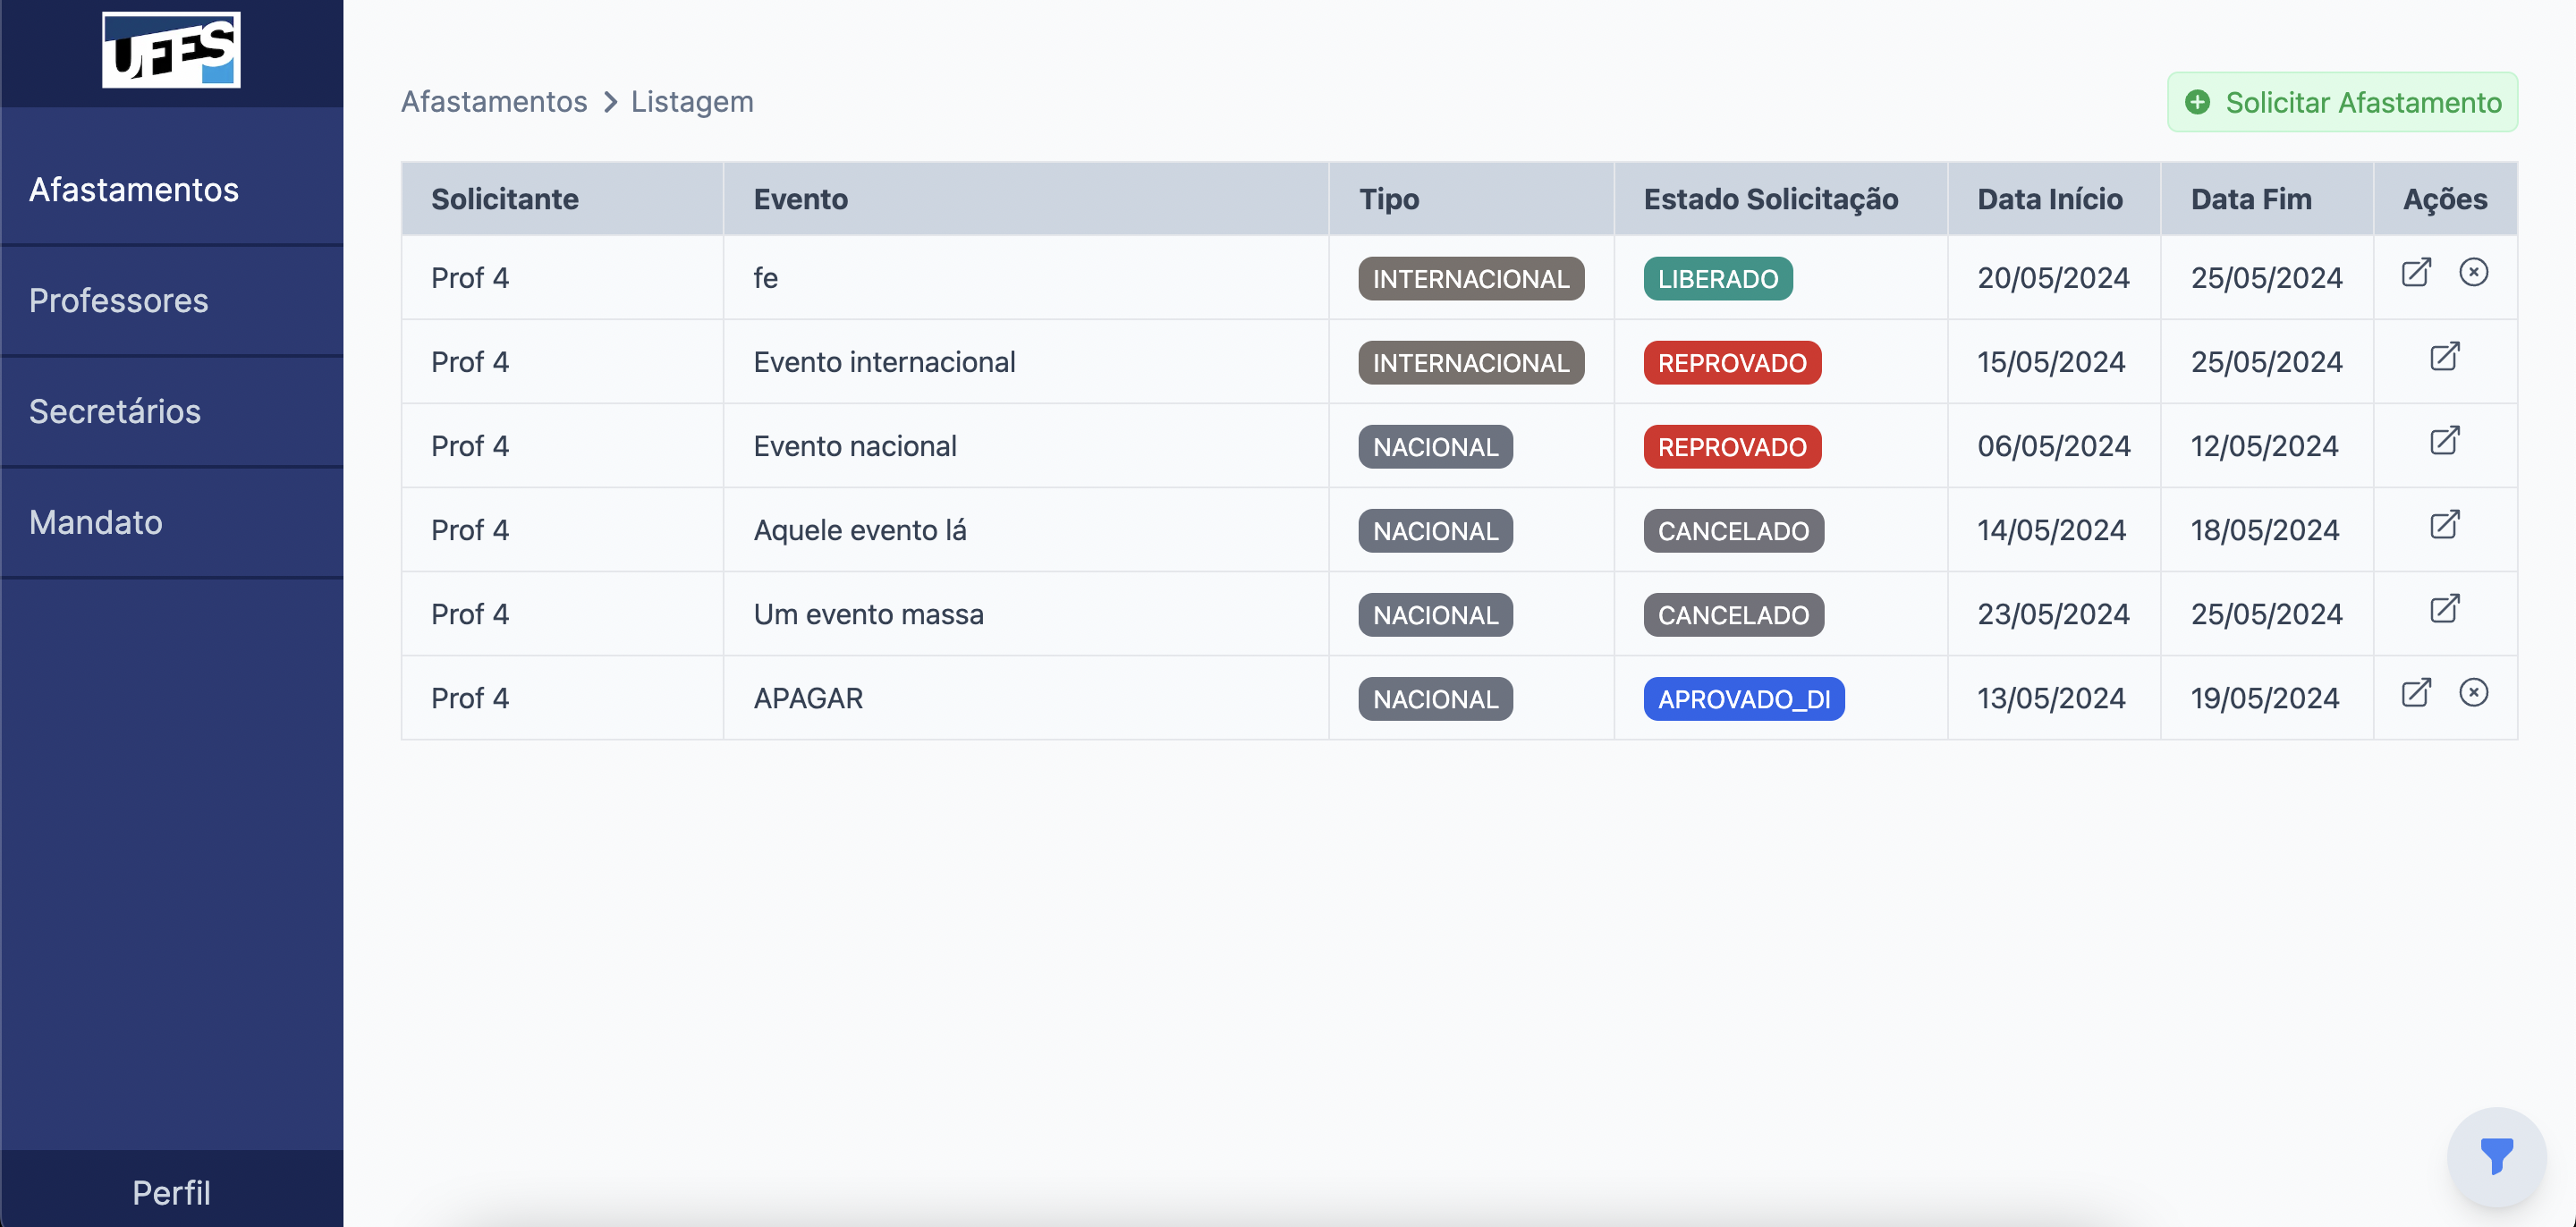
\includegraphics[width=\textwidth]{figuras/prints-app/fig-lista-afastamento.png}
    \caption{Listagem de Afastamentos do SCAP.}
    \label{fig-listagem-afastamentos}
\end{figure}

\begin{figure}[h!]
    \centering
    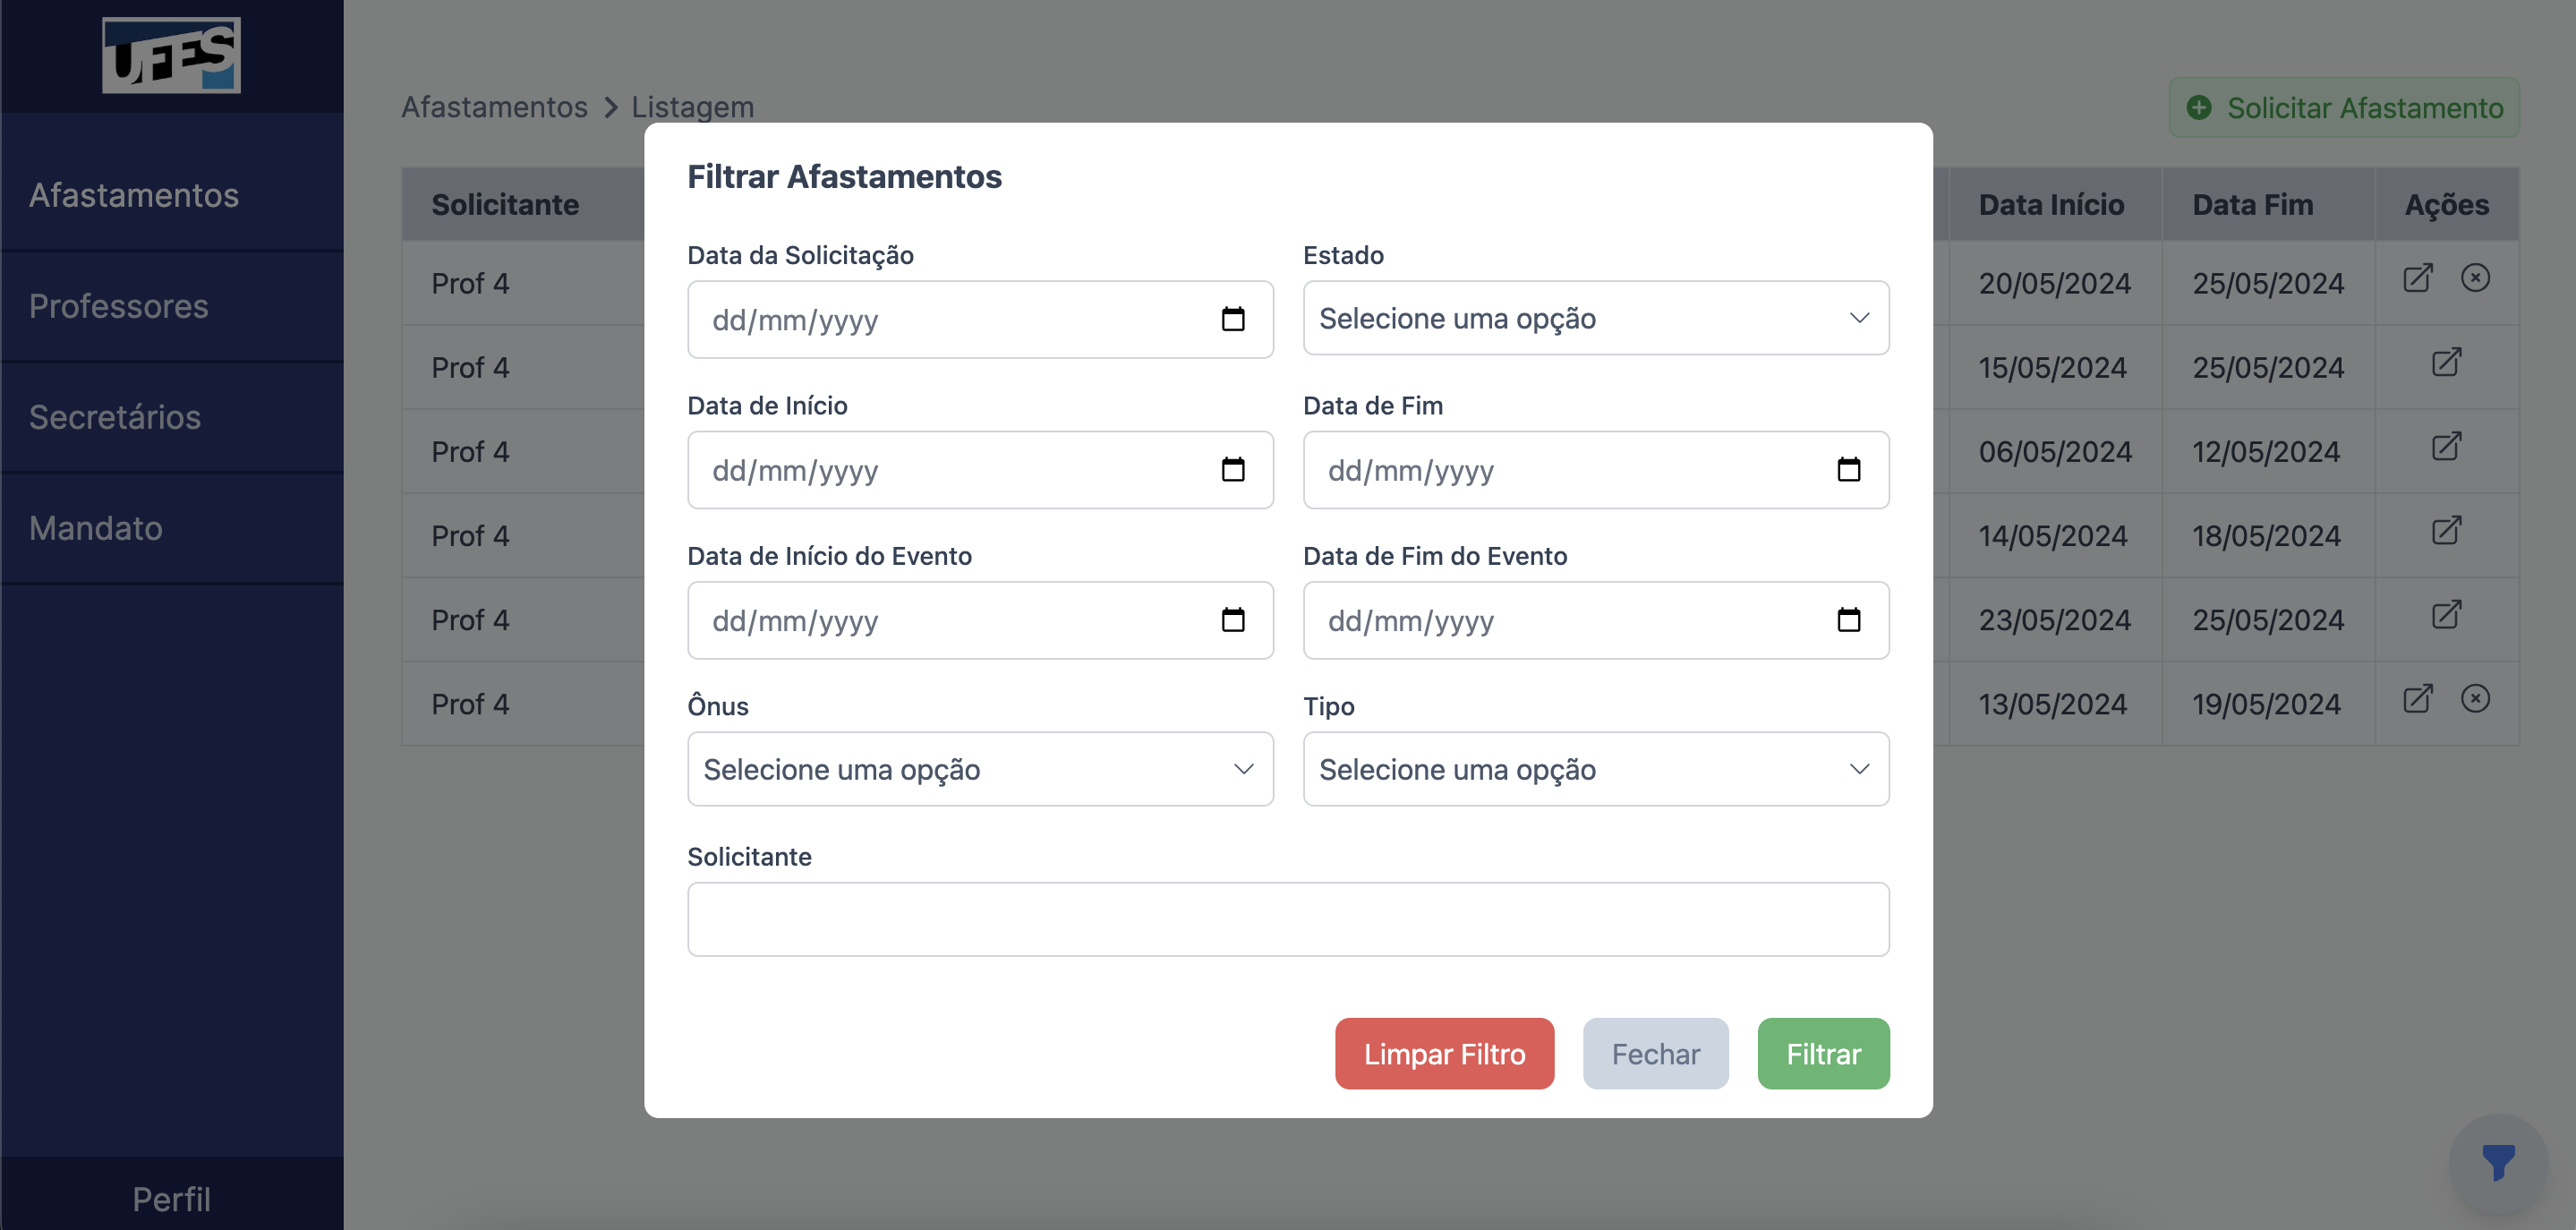
\includegraphics[width=\textwidth]{figuras/prints-app/fig-filtro-afastamento.png}
    \caption{Filtro de Busca de Afastamentos.}
    \label{fig-filtro-afastamentos}
\end{figure}

\subsection{Cadastro de Afastamento}
\label{subsec-projeto-cadastro-afastamento}

A Figura~\ref{fig-cadastro-afastamento} apresenta a tela de cadastro de afastamento do SCAP. Esta rota
é acessível apenas para professores, que podem solicitar um afastamento preenchendo o formulário,
campos marcados com asterisco são obrigatórios. 

\begin{figure}[h!]
    \centering
    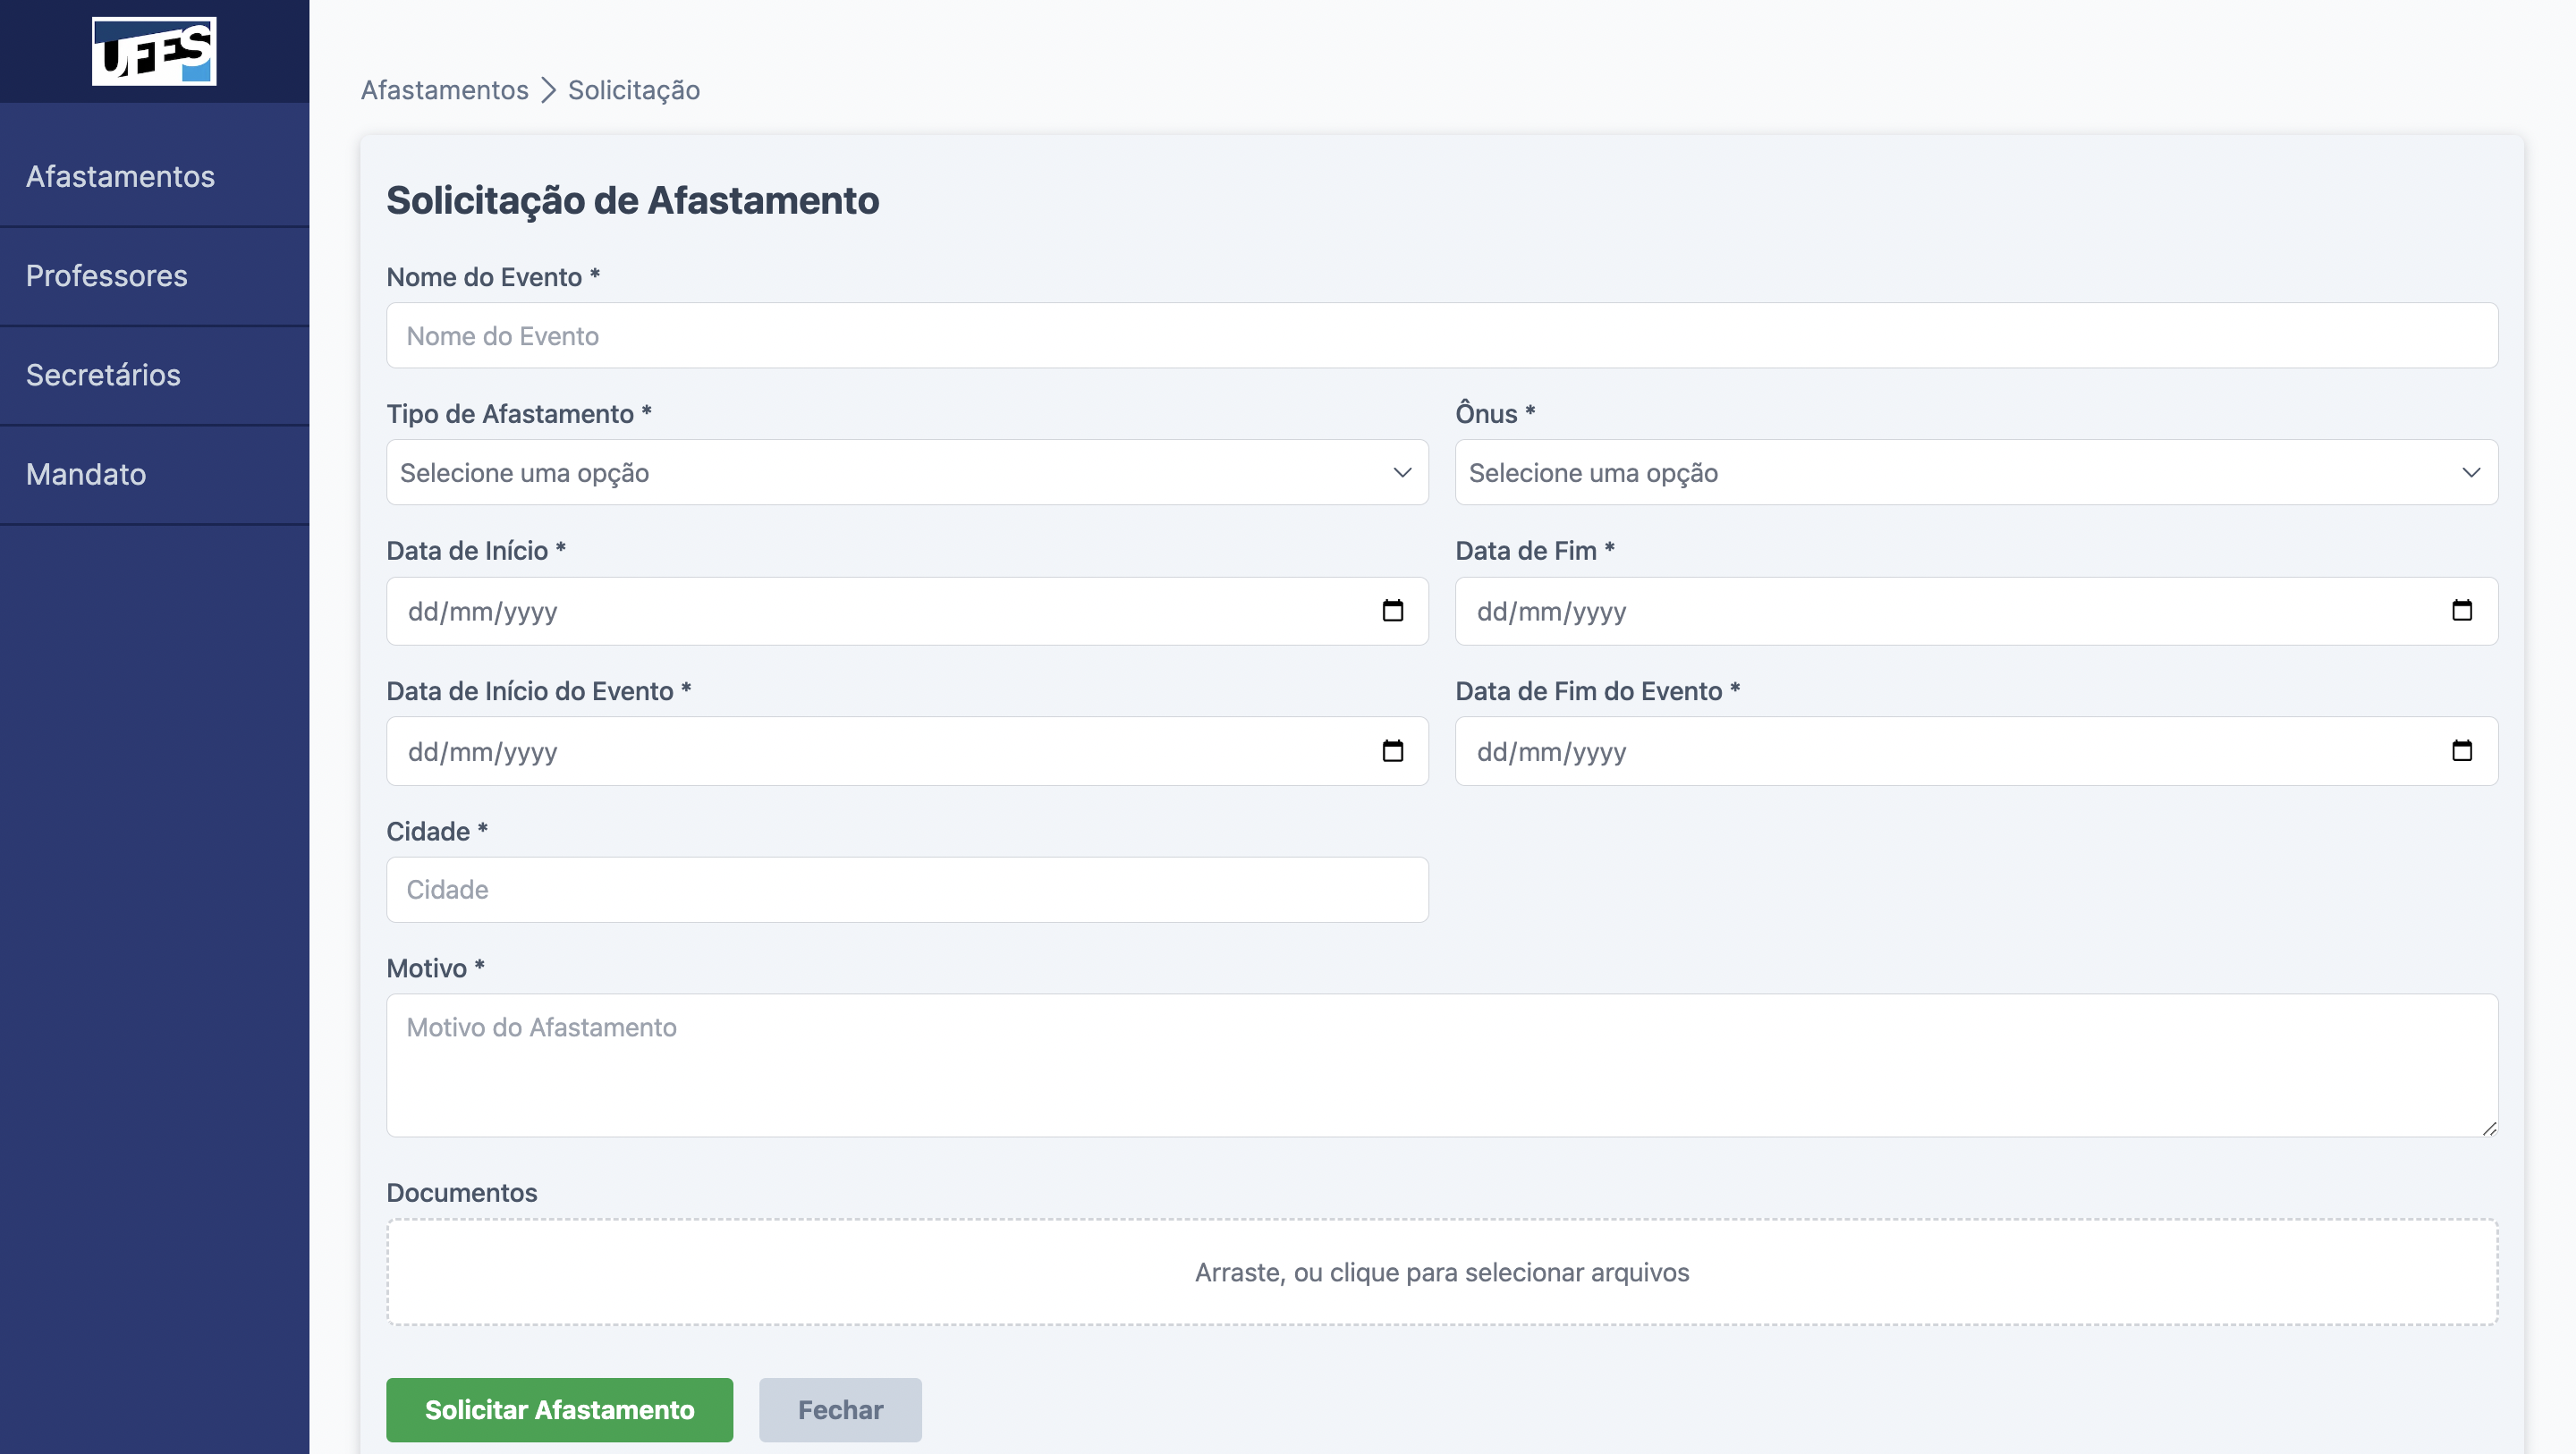
\includegraphics[width=\textwidth]{figuras/prints-app/fig-solicitar-afastamento.png}
    \caption{Cadastro de Afastamento do SCAP.}
    \label{fig-cadastro-afastamento}
\end{figure}

A edição de um afastamento é feita de forma similar ao cadastro, porém os campos já estarão preenchidos com os valores
do afastamento a ser editado. O mesmo componente é utilizado para ambas as ações, estando a diferença na rota acessada.
Na edição, apenas o professor solicitante pode editar as informações do afastamento, exceto os campos:
\textit{estado} e \textit{relator}, que são de responsabilidade do secretário e professor chefe, respectivamente. Um exemplo é exibido na Figura~\ref{fig-editar-afastamento}.

\begin{figure}
    \centering
    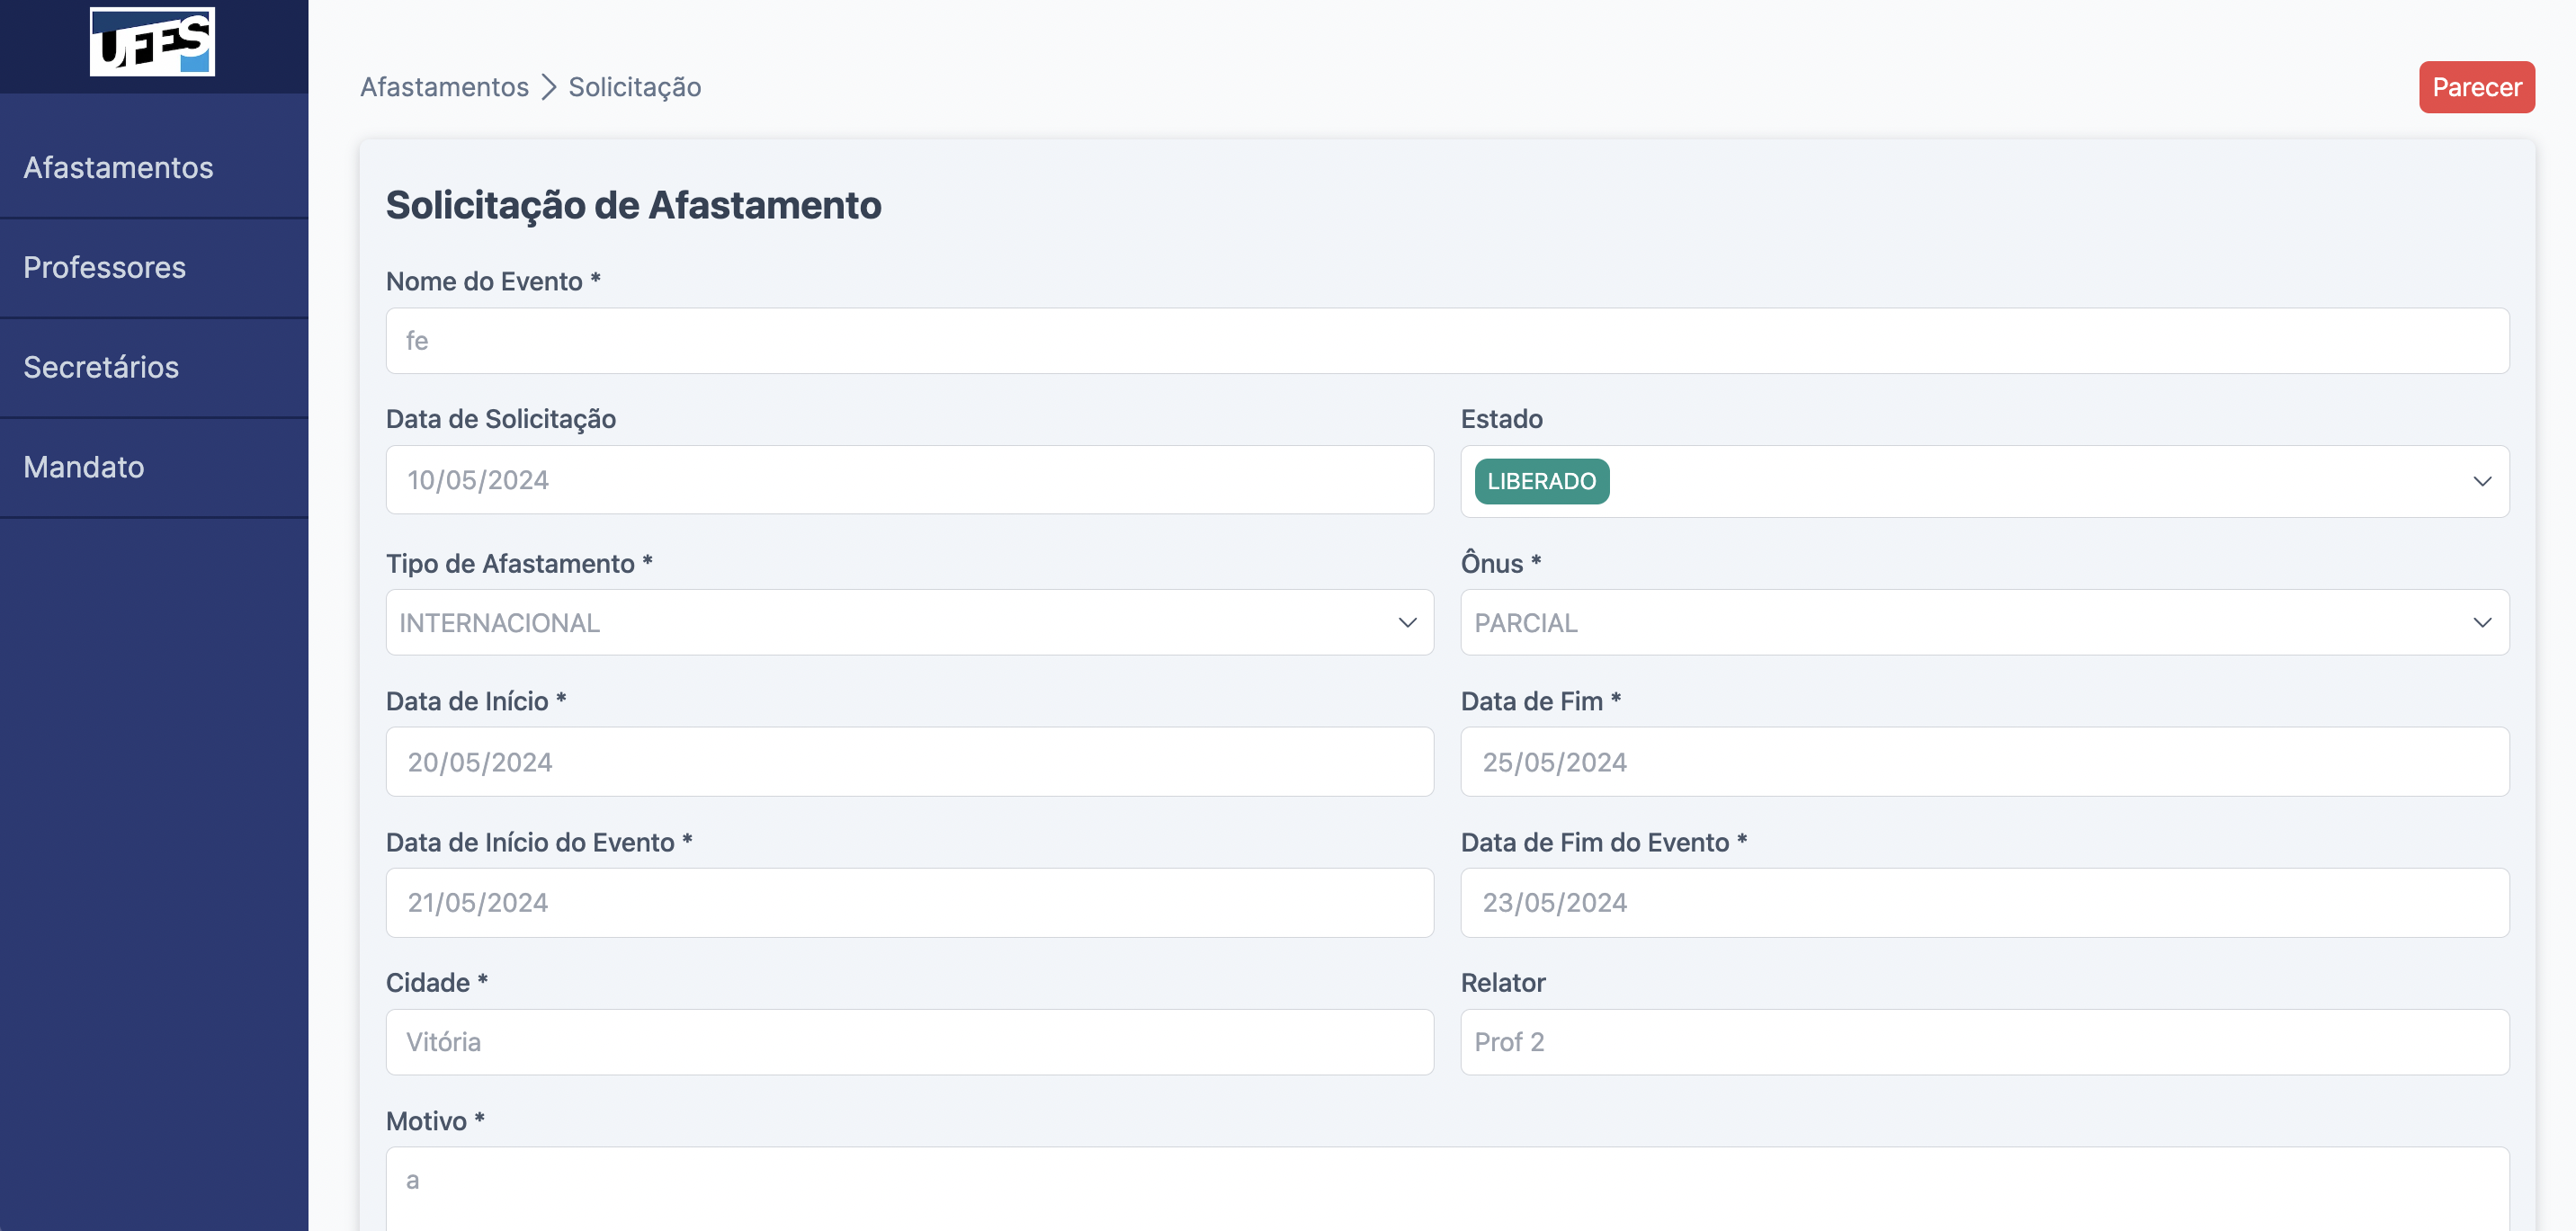
\includegraphics[width=\textwidth]{figuras/prints-app/fig-editar-afastamento.png}
    \caption{Edição de Afastamento do SCAP.}
    \label{fig-editar-afastamento}
\end{figure}

Caso seja um professor sem parentesco com o solicitante do afastamento, o botão de \textbf{Parecer} estará disponível,
abrindo um modal com o formulário para preenchimento do parecer. A Figura~\ref{fig-parecer} apresenta este modal.
Por serem funcionalidades semelhantes, o modal de parecer é utilizado também para pareceres externos (CT e PRPPG) e manifestações
de professores contra o afastamento nacional.

\begin{figure}
    \centering
    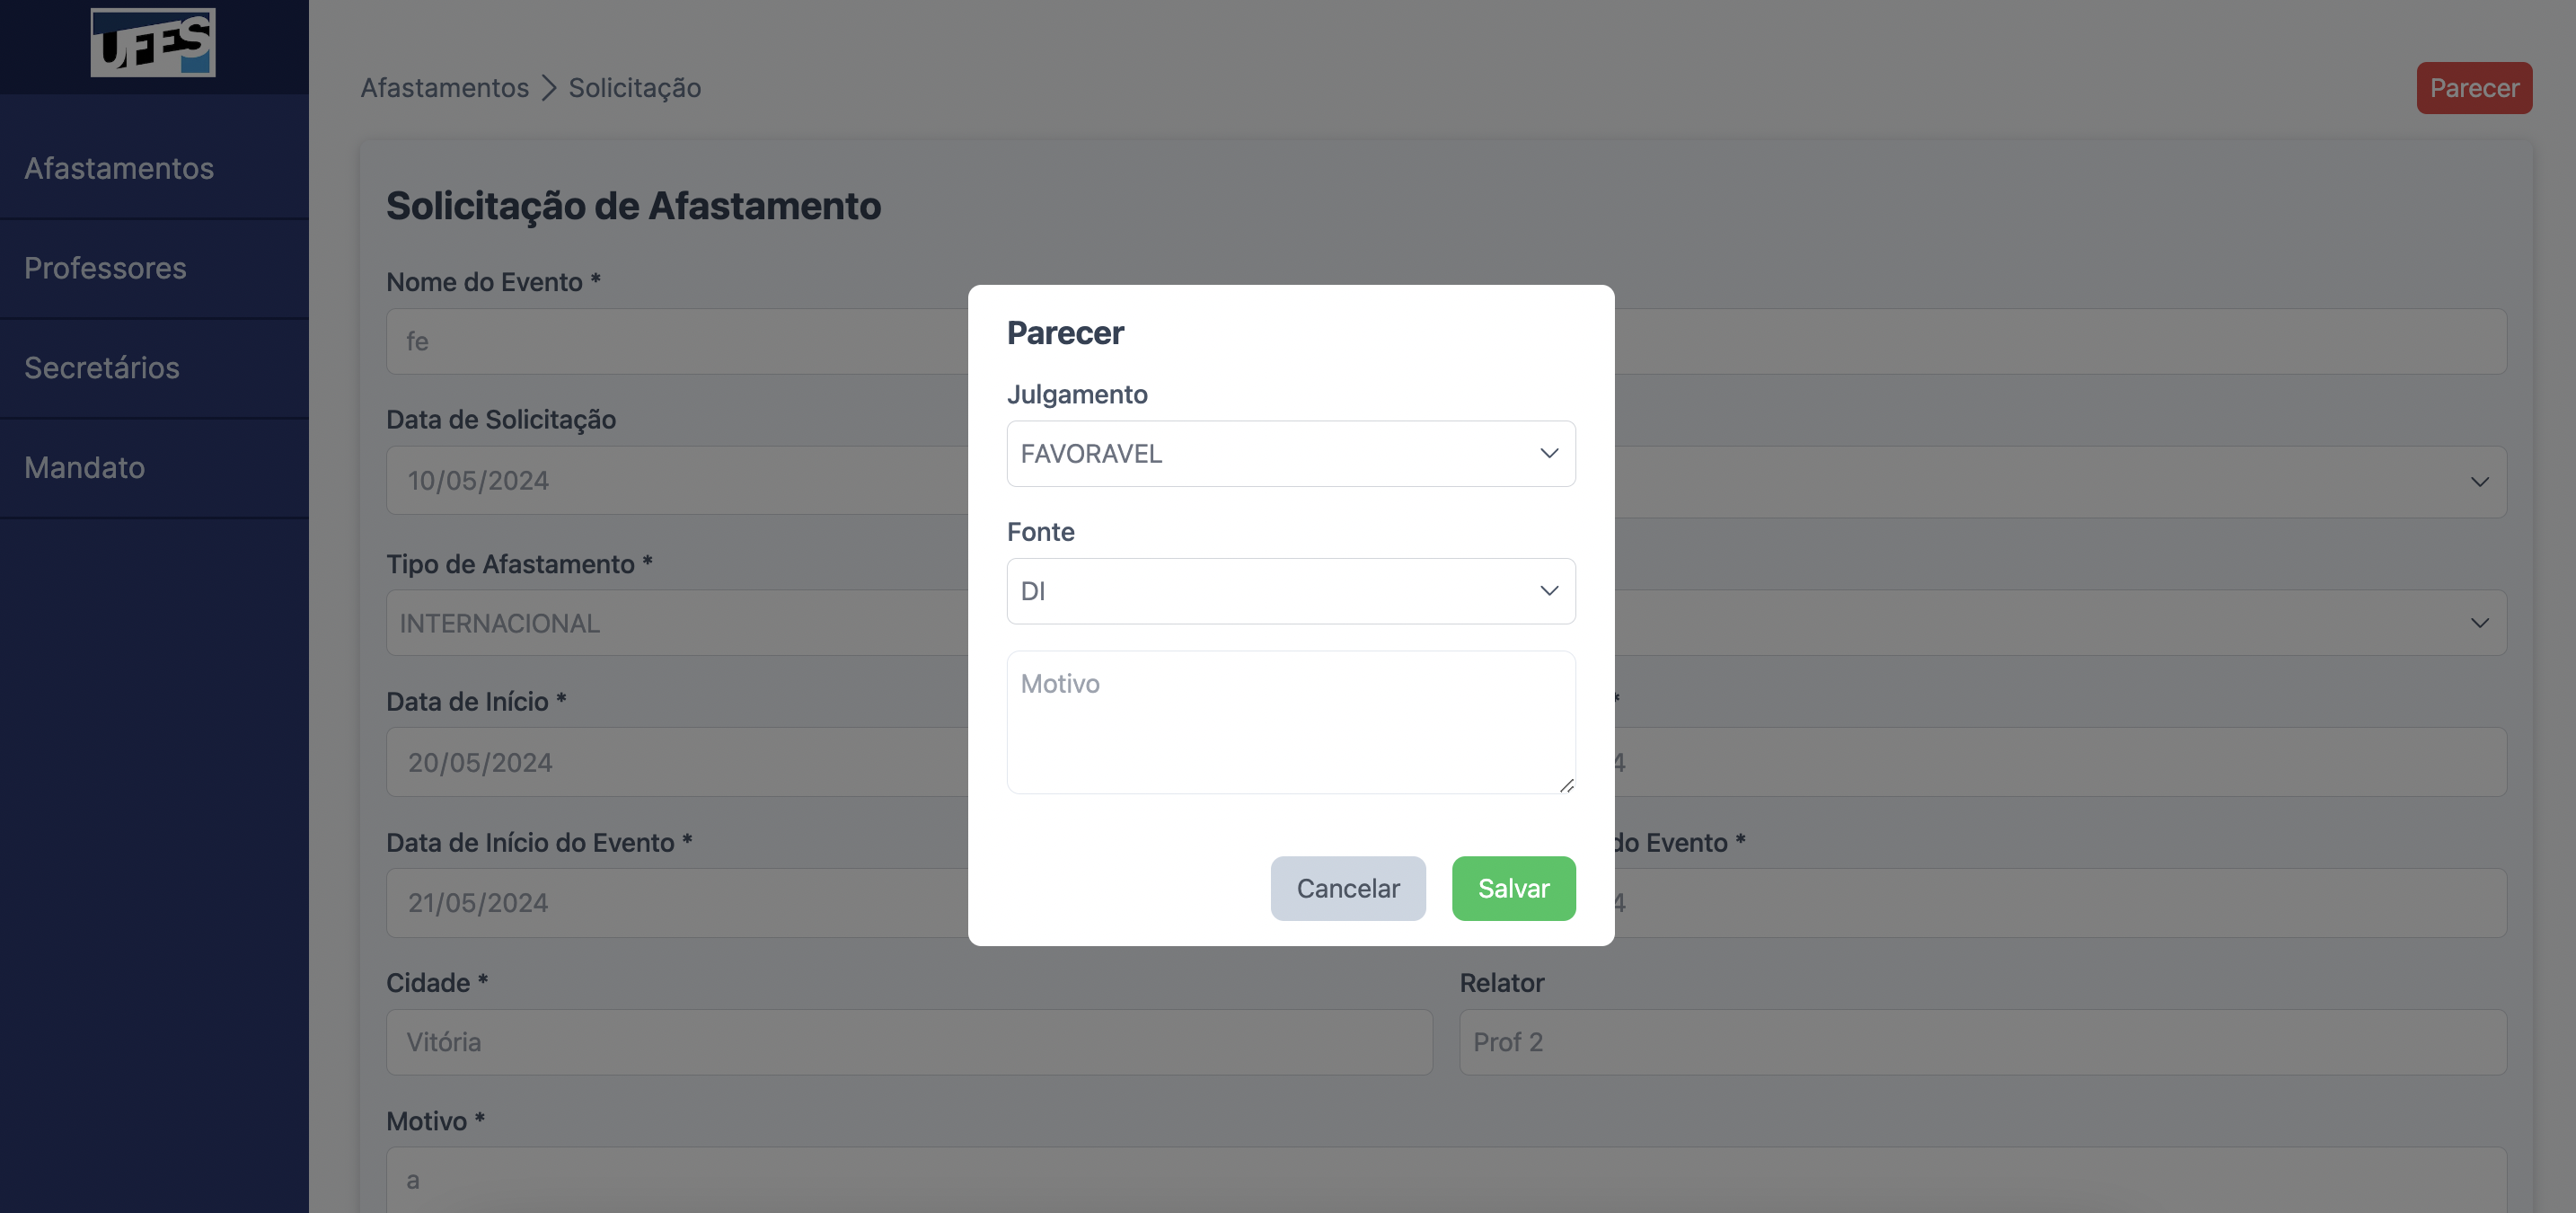
\includegraphics[width=\textwidth]{figuras/prints-app/fig-parecer.png}
    \caption{Modal de Parecer do SCAP.}
    \label{fig-parecer}
\end{figure}

Por fim, o formulário de afastamento possui também um campo para \textit{upload} de arquivos, onde o professor solicitante
pode anexar o relatório de viagem e o secretário pode anexar atas ou documentos enviados pelo CT e PRPPG.

\subsection{Cadastro de Usuários}
\label{subsec-projeto-cadastro-usuarios}

Através do \textbf{NavBar} é possível navegar pela aplicação, clicando em \textbf{Professores} o usuário é redirecionado
para a página de listagem de professores, onde é possível visualizar os professores cadastrados, assim como seus \textit{e-mails}
e telefones. A Figura~\ref{fig-listagem-professores} apresenta a tela de listagem de professores do SCAP.

\begin{figure}[h!]
    \centering
    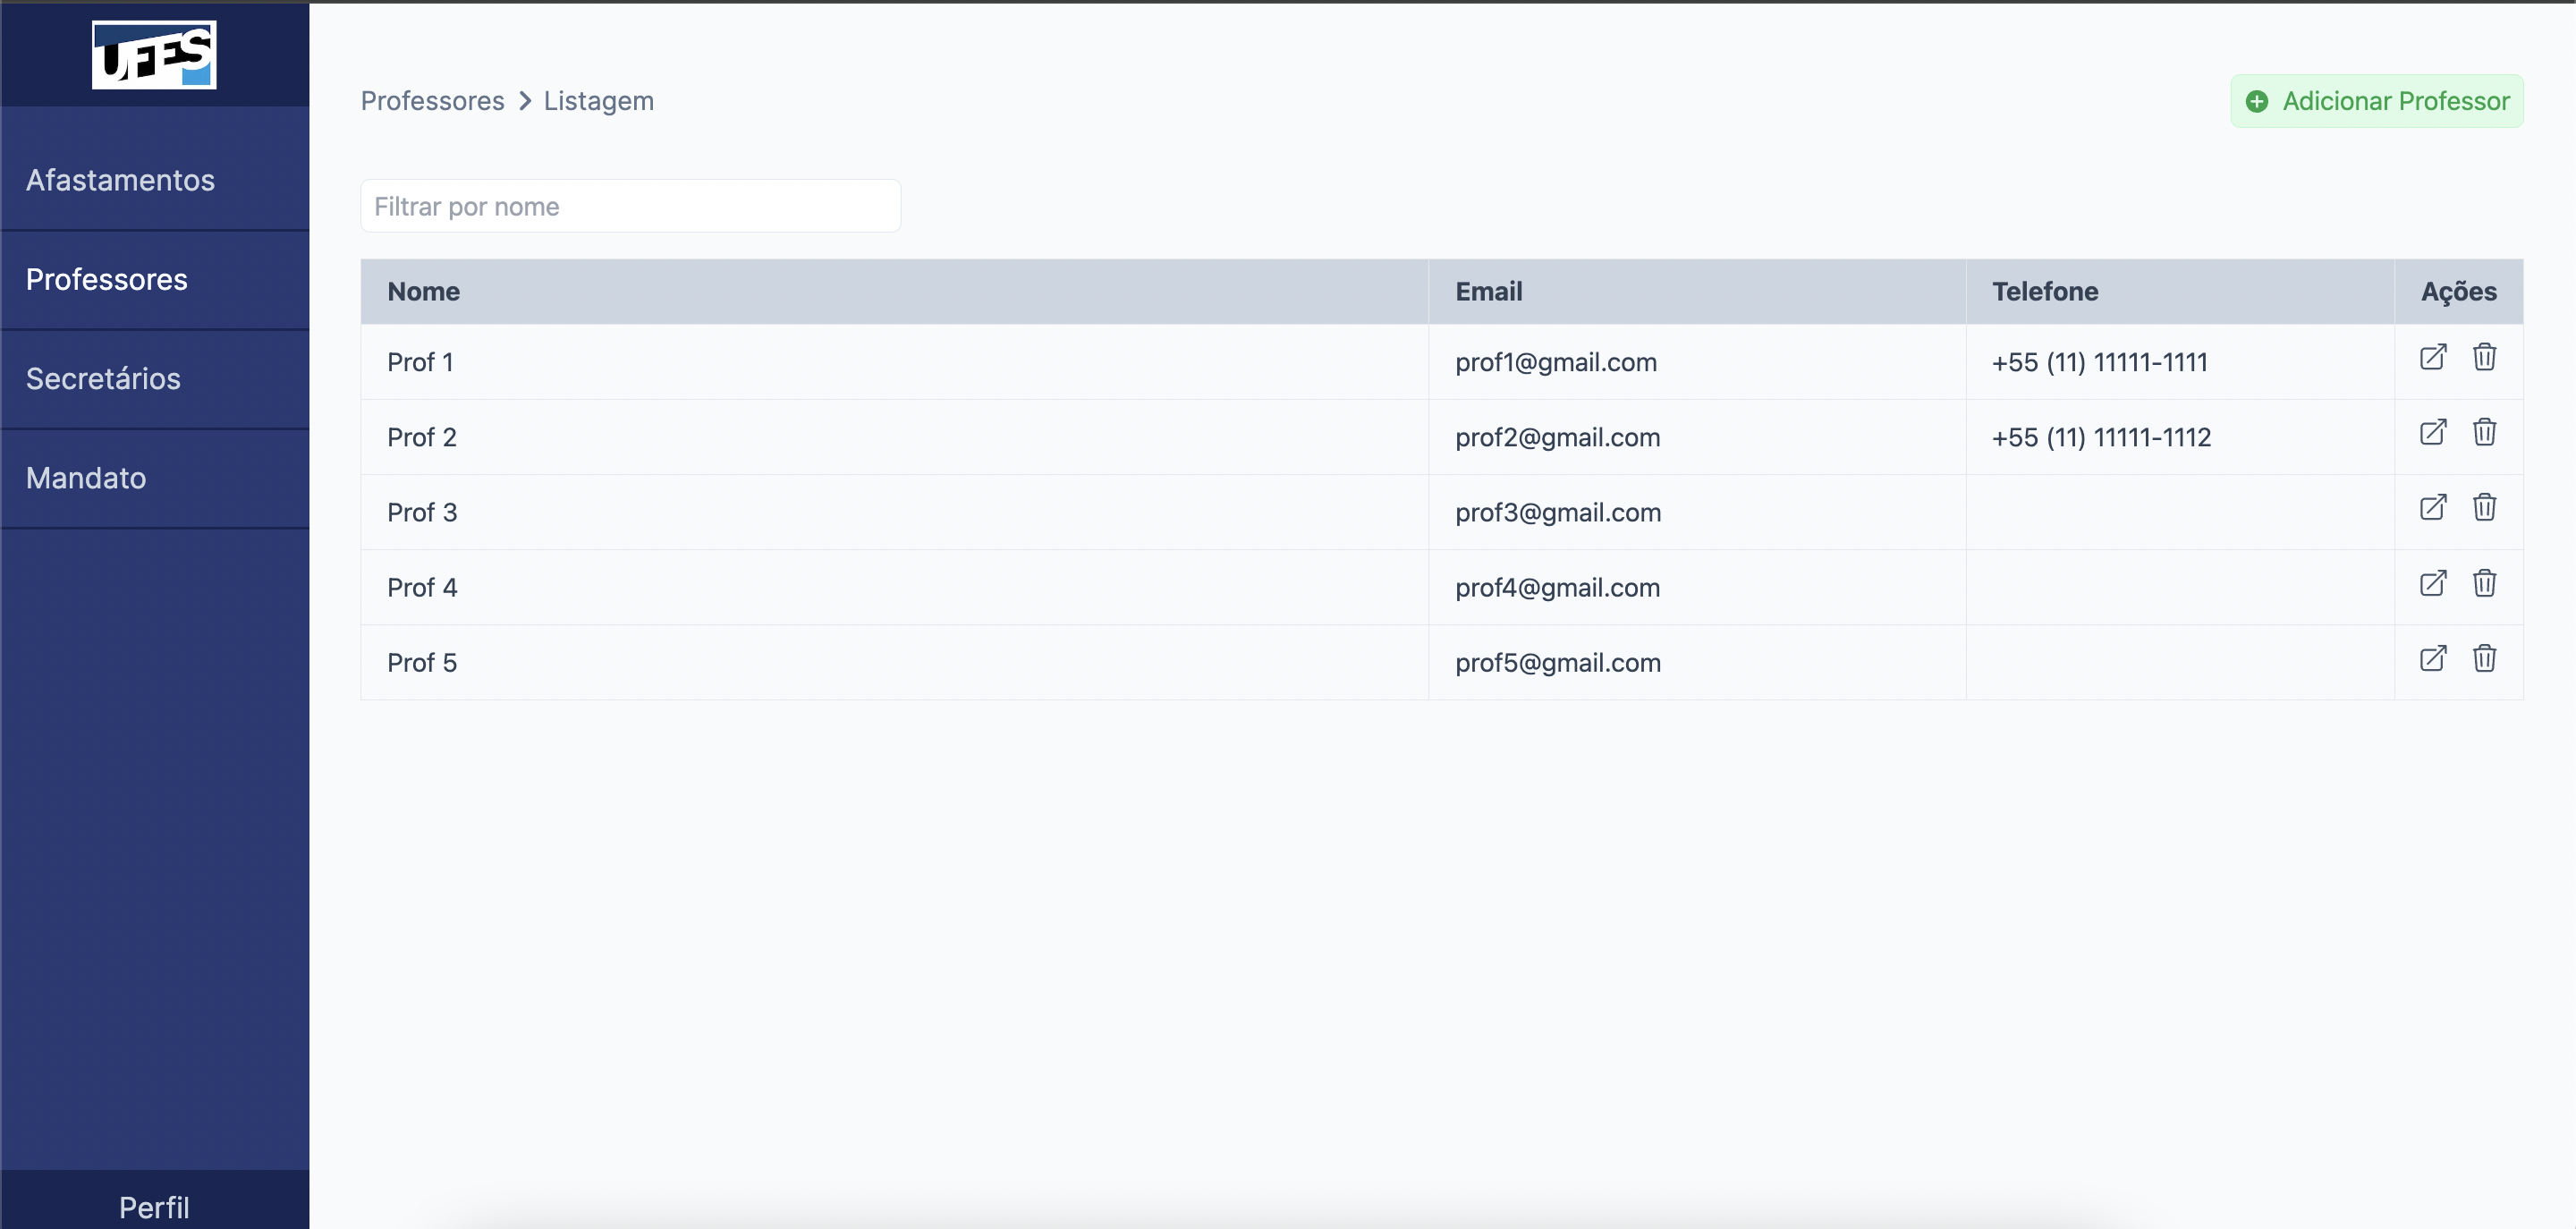
\includegraphics[width=\textwidth]{figuras/prints-app/fig-lista-professor.png}
    \caption{Listagem de Professores do SCAP.}
    \label{fig-listagem-professores}
\end{figure}

A Figura~\ref{fig-listagem-secretarios} apresenta a tela de listagem de secretários, que pode ser acessada
da mesma forma, pelo \textbf{NavBar} clicando em \textbf{Secretários}.

\begin{figure}[h!]
    \centering
    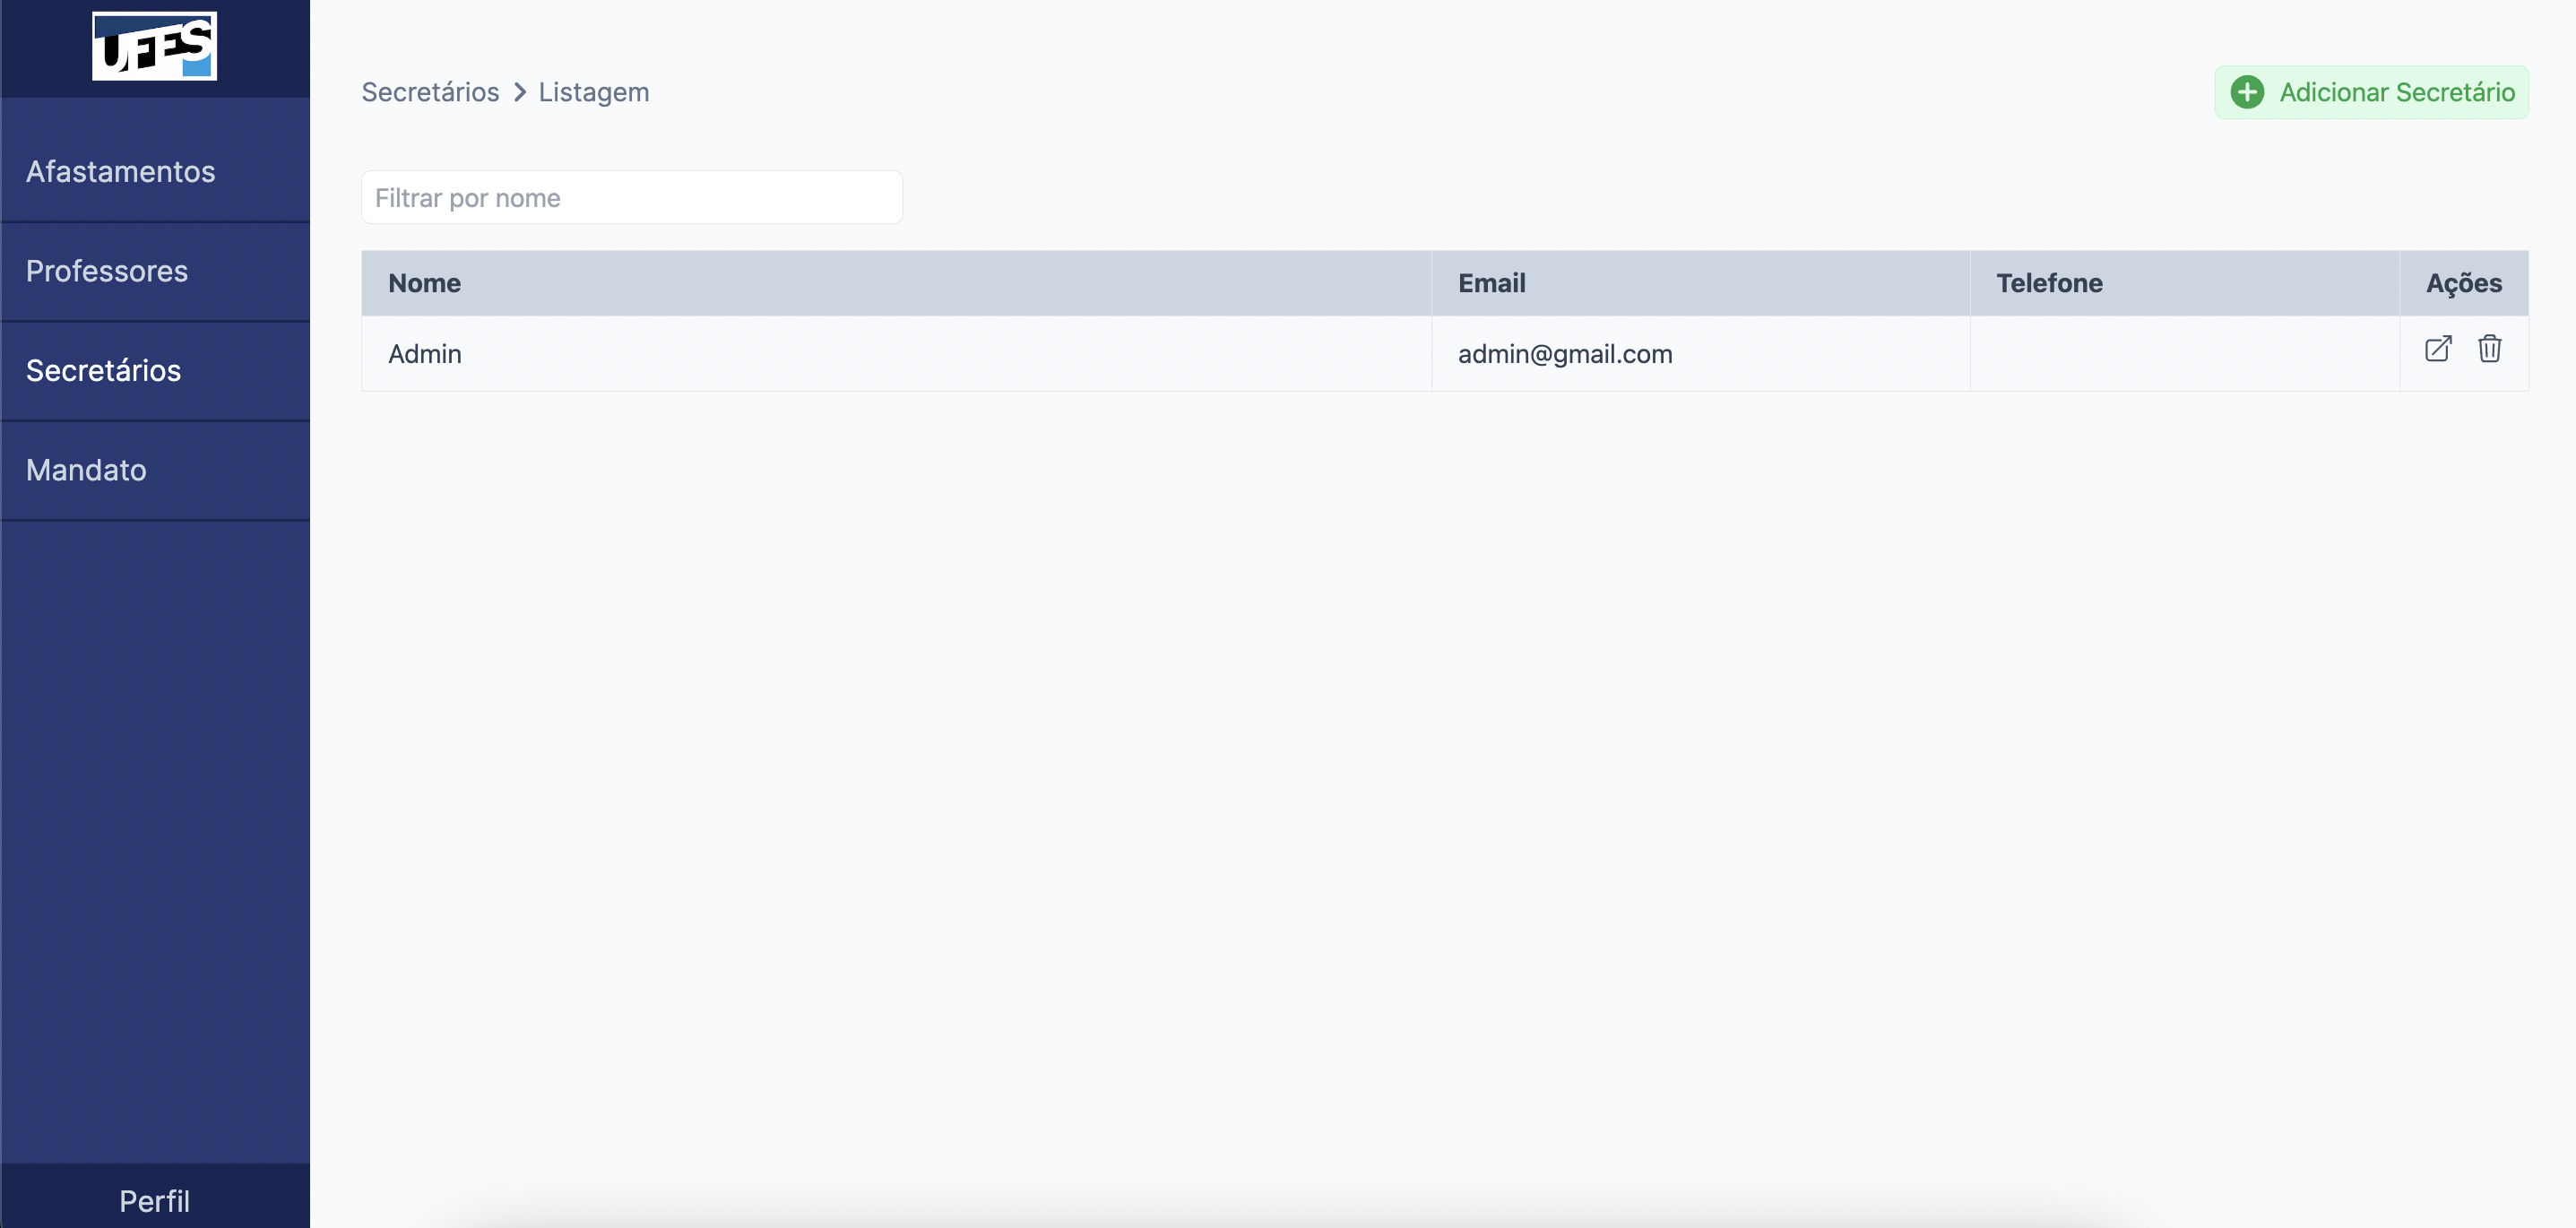
\includegraphics[width=\textwidth]{figuras/prints-app/fig-lista-secretario.png}
    \caption{Listagem de Secretários do SCAP.}
    \label{fig-listagem-secretarios}
\end{figure}

Apenas o secretário pode deletar, visualizar e adicionar professores. A Figura~\ref{fig-cadastro-professor} apresenta
a tela de cadastro de usuários, por onde o secretário pode adicionar um novo usuário preenchendo o formulário,
seja ele um professor ou secretário. Campos marcados com asterisco são obrigatórios.

\begin{figure}[h!]
    \centering
    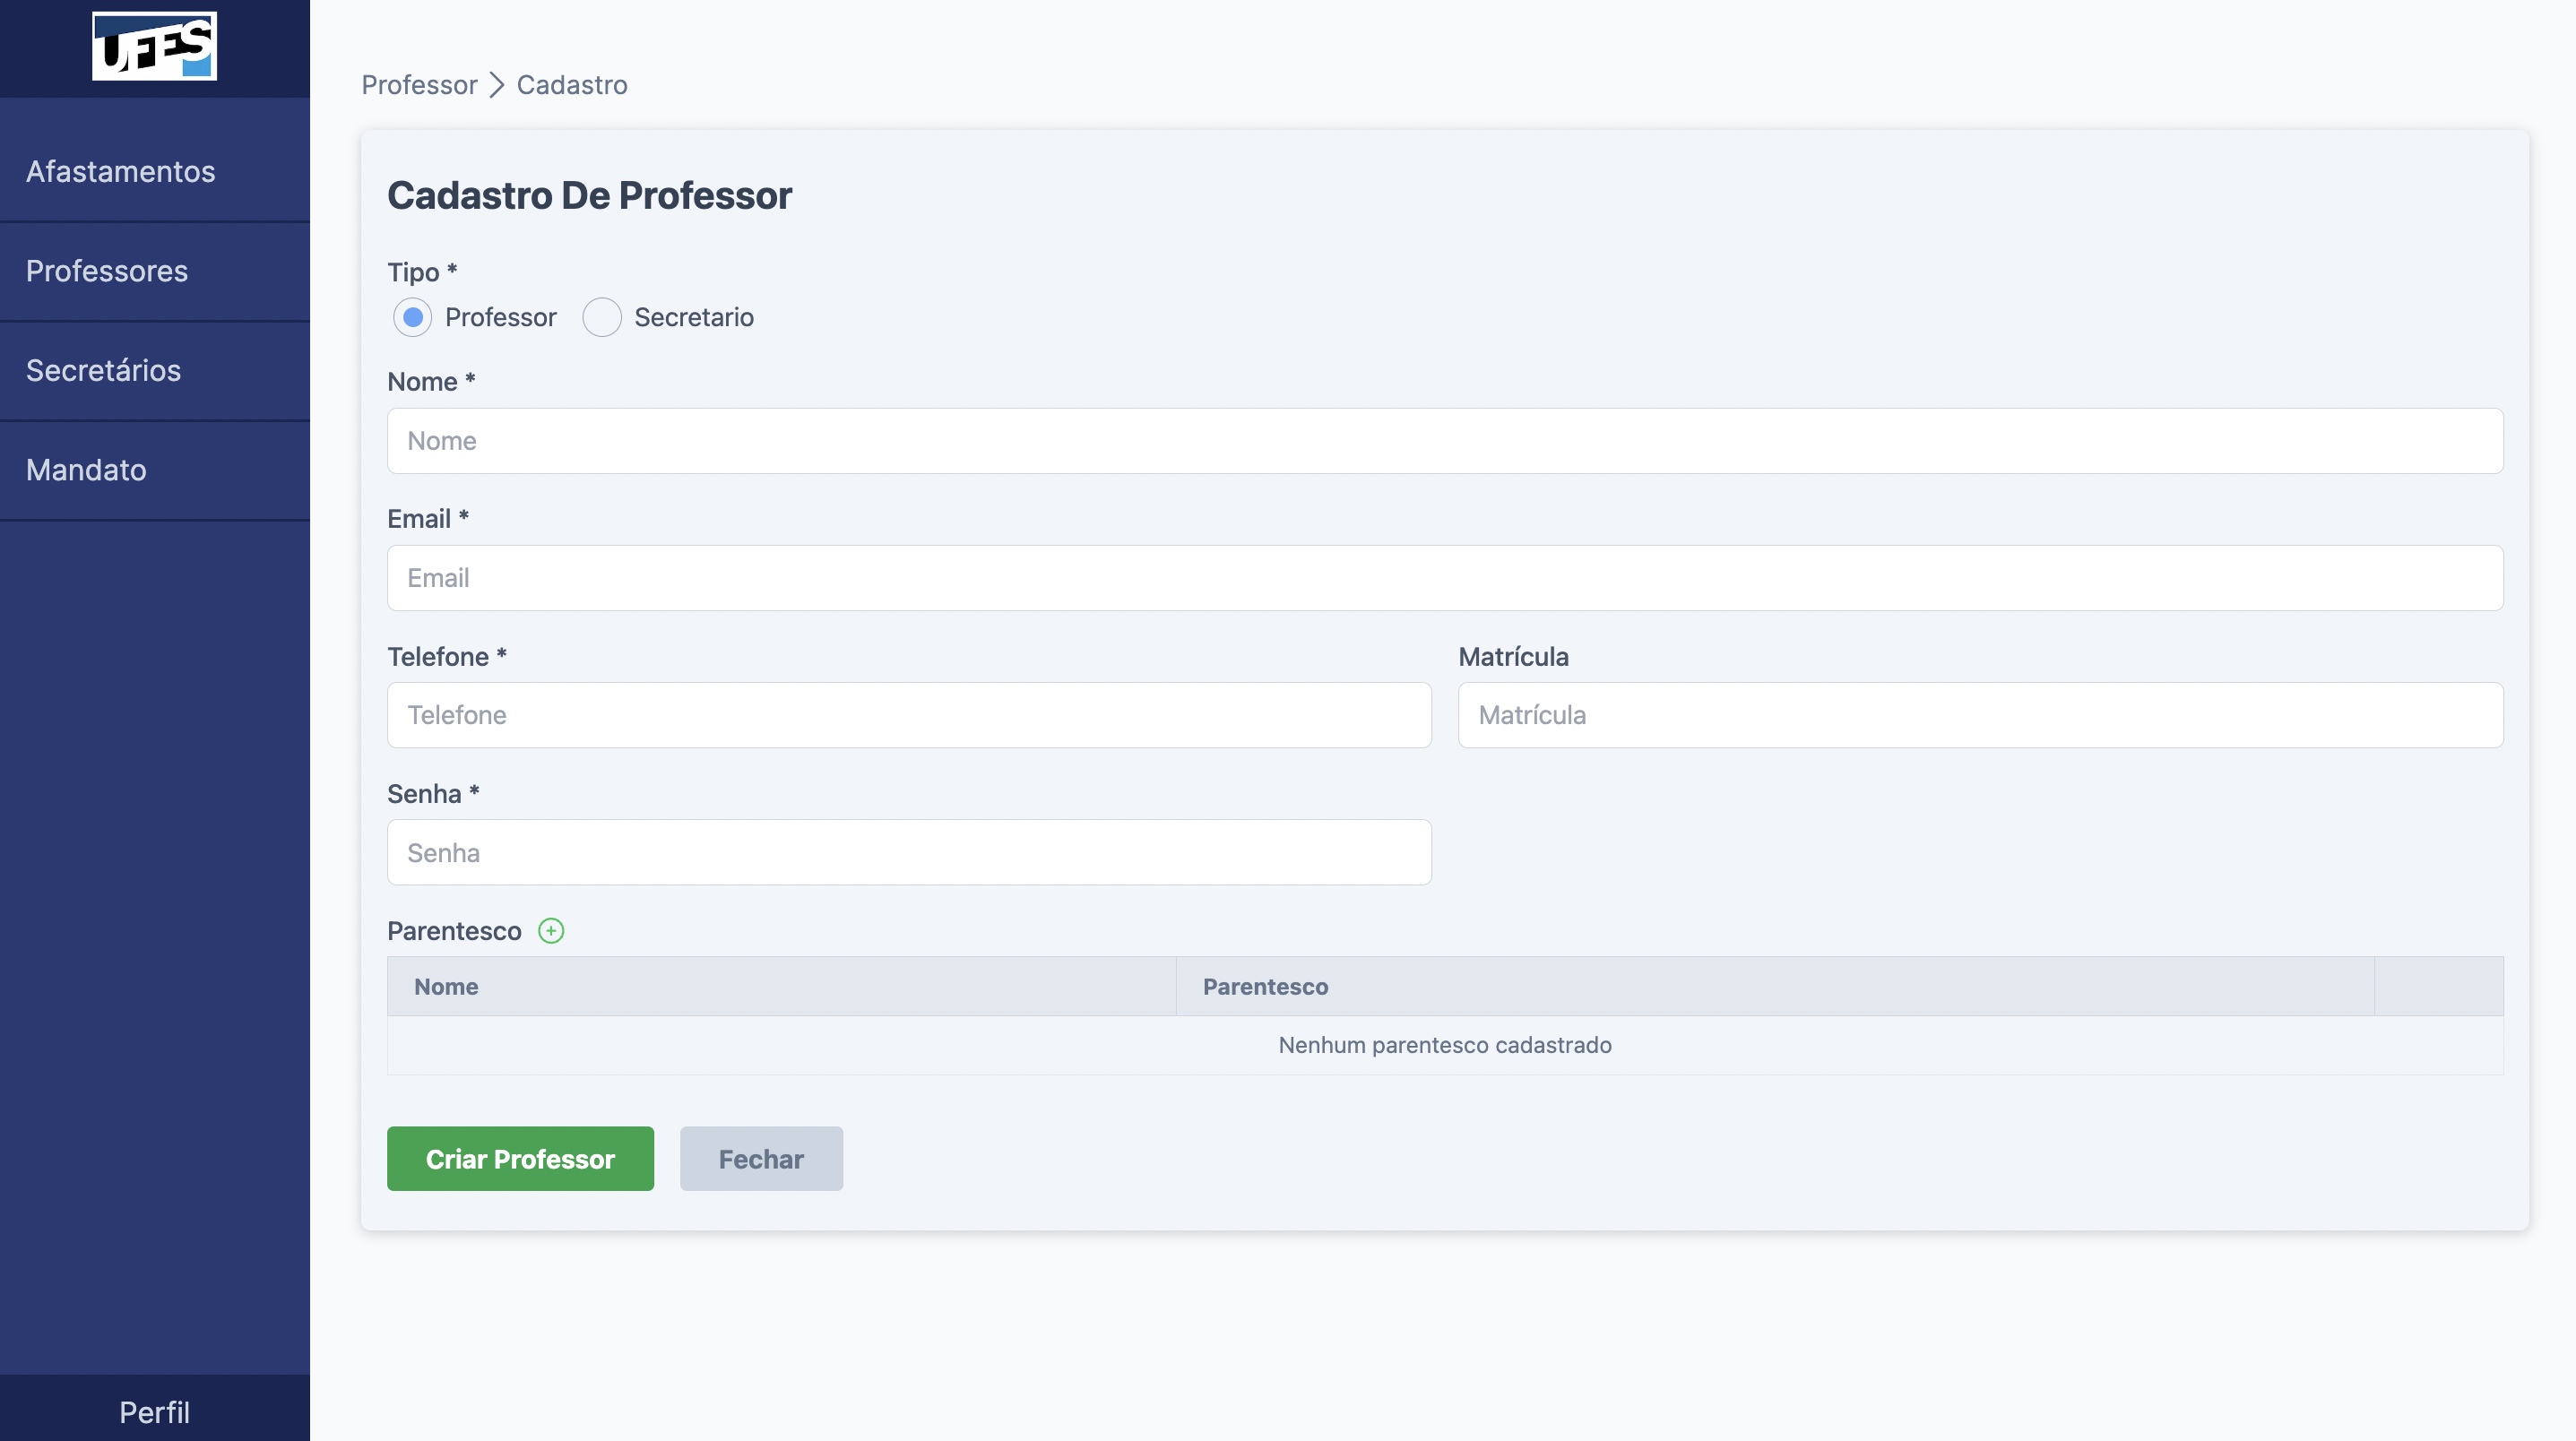
\includegraphics[width=\textwidth]{figuras/prints-app/fig-cadastro-professor.png}
    \caption{Cadastro de Usuários do SCAP.}
    \label{fig-cadastro-professor}
\end{figure}


Caso o usuário a ser criado seja um professor, o secretário pode adicionar parentescos entre professores.
Para isso, deve-se clicar no botão de adição que então abre um modal com um pequeno formulário.
A Figura~\ref{fig-parentesco} apresenta este modal.


\begin{figure}
    \centering
    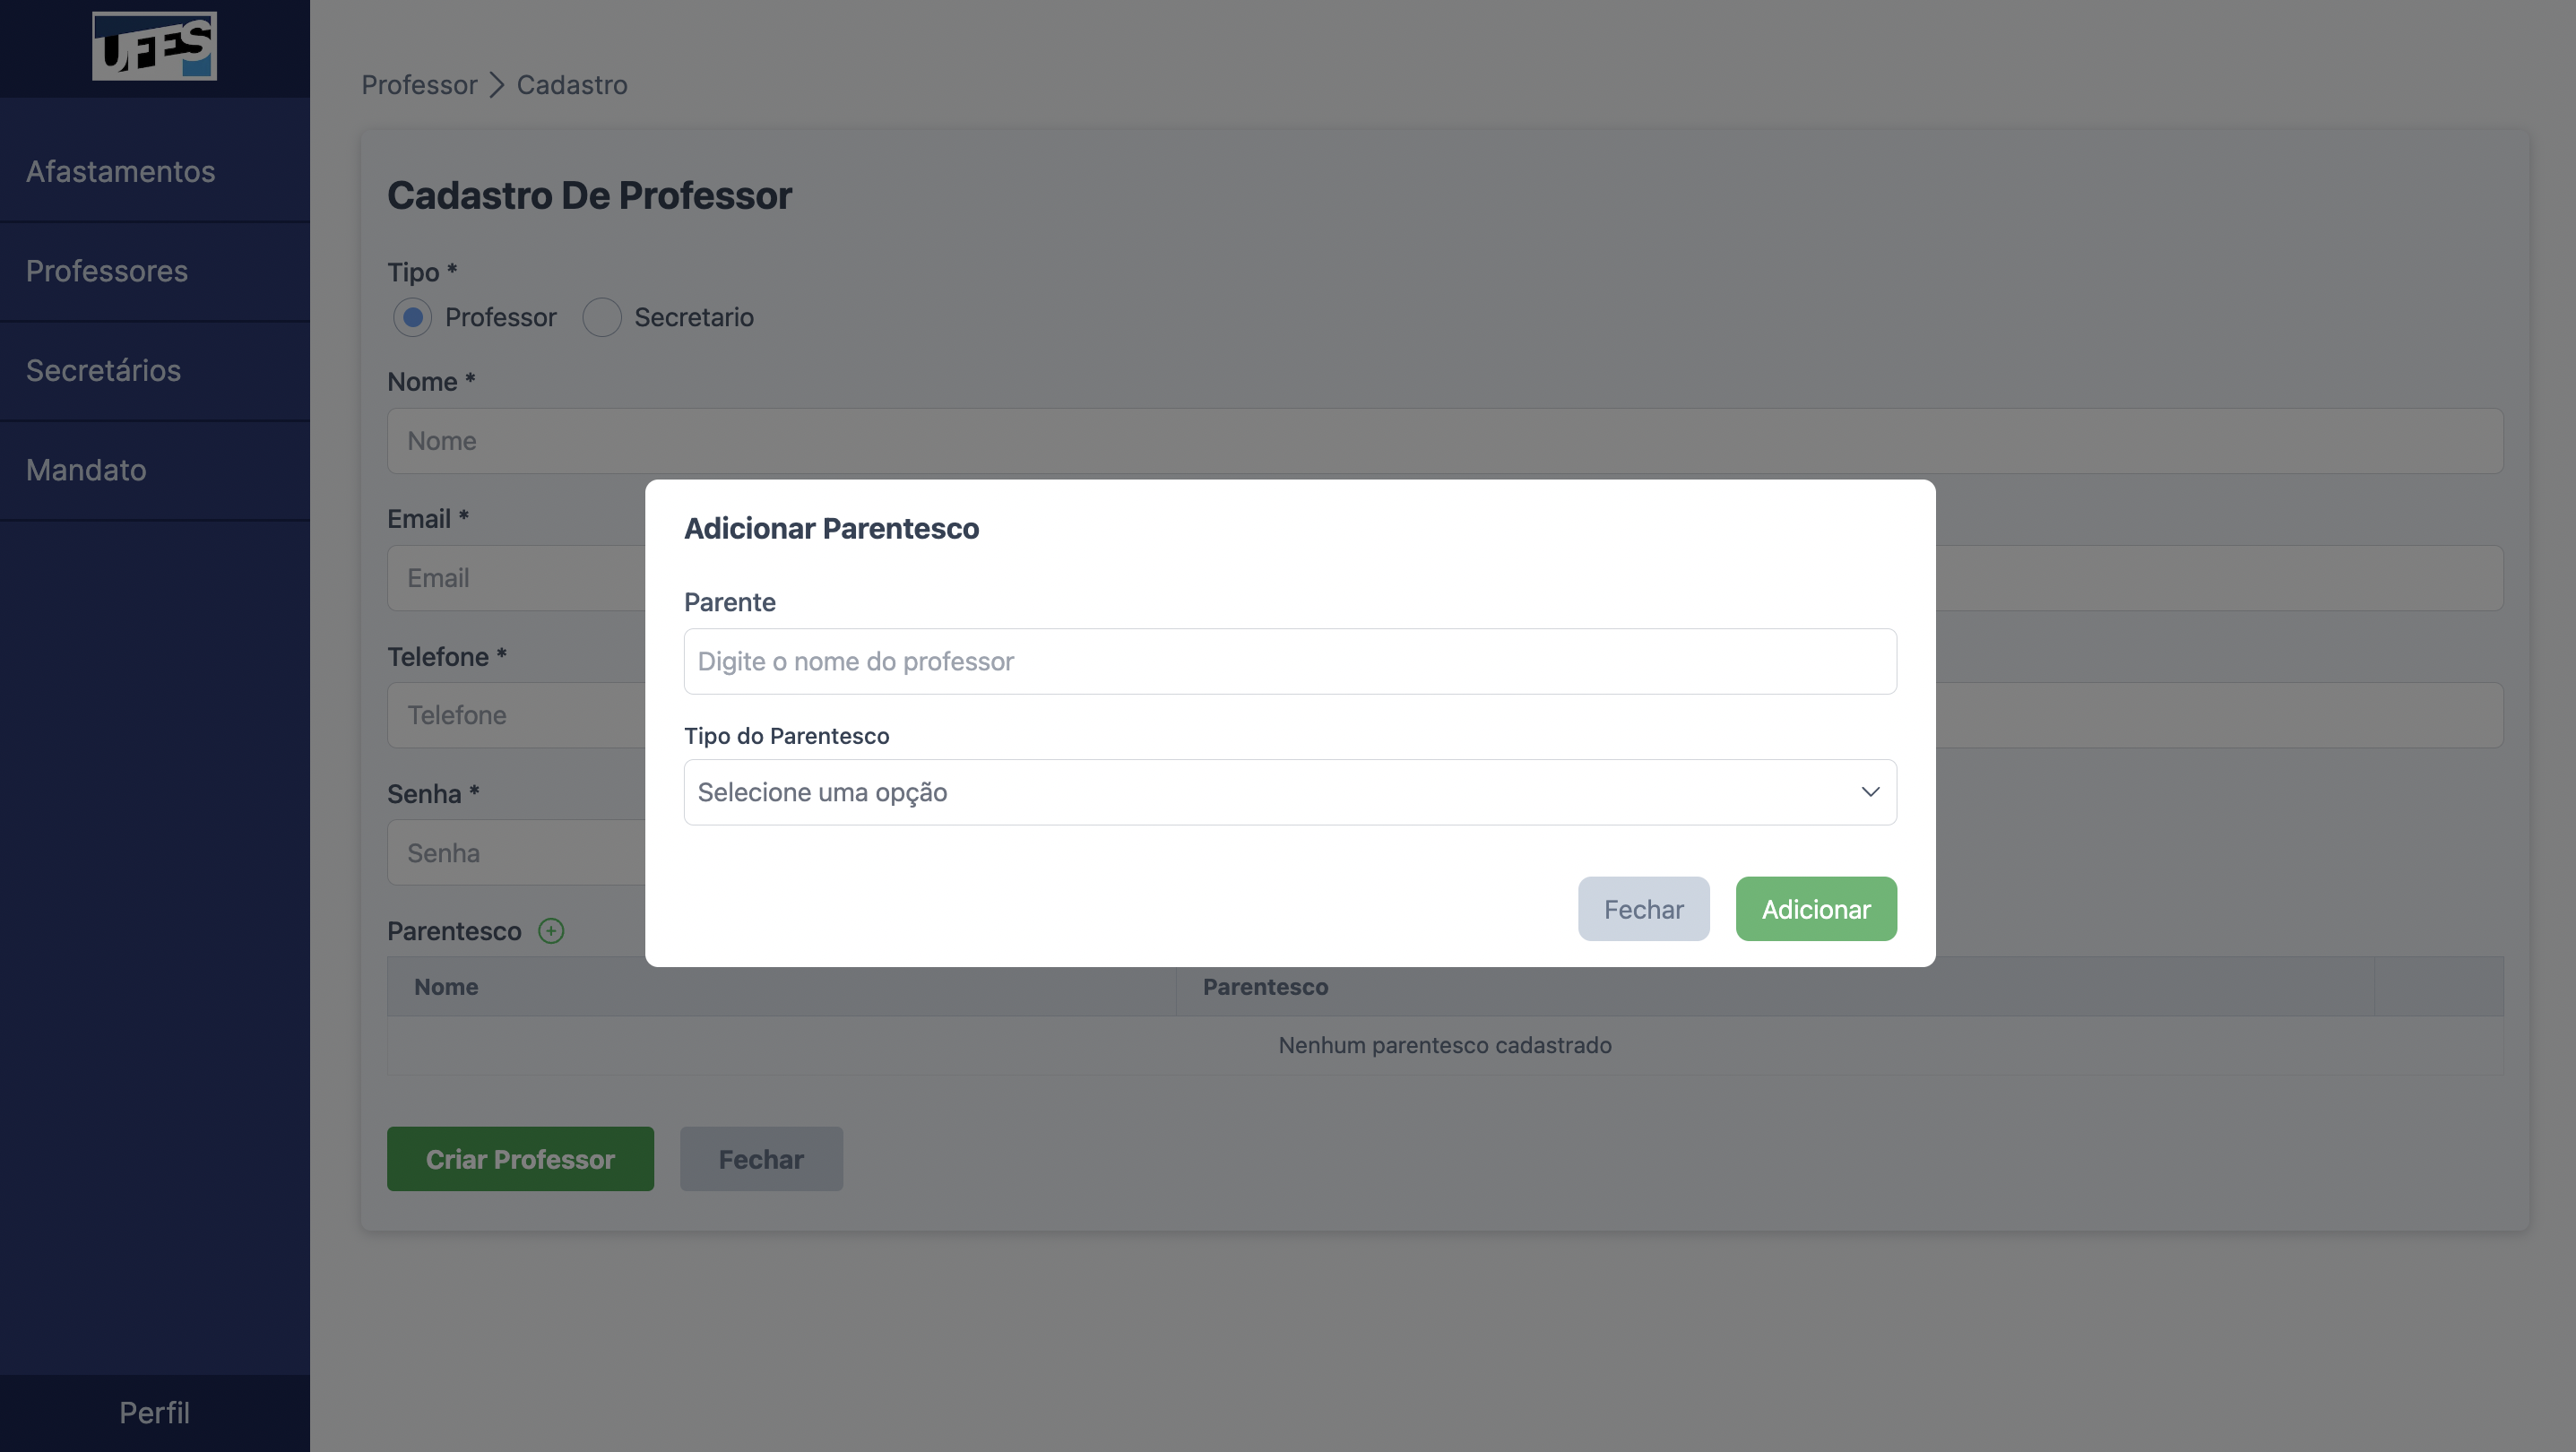
\includegraphics[width=\textwidth]{figuras/prints-app/fig-modal-parentesco.png}
    \caption{Cadastro de Parentesco do SCAP.}
    \label{fig-parentesco}
\end{figure}


O componente de cadastro de usuários é utilizado também para a edição de usuários, assim como foi feito com Afastamentos. A Figura~\ref{fig-editar-professor}
apresenta a página de usuário preenchida com os dados do professor logado no momento. É por essa página também que o usuário pode alterar sua senha ou realizar o \textit{logout} do sistema.

\begin{figure}[h!]
    \centering
    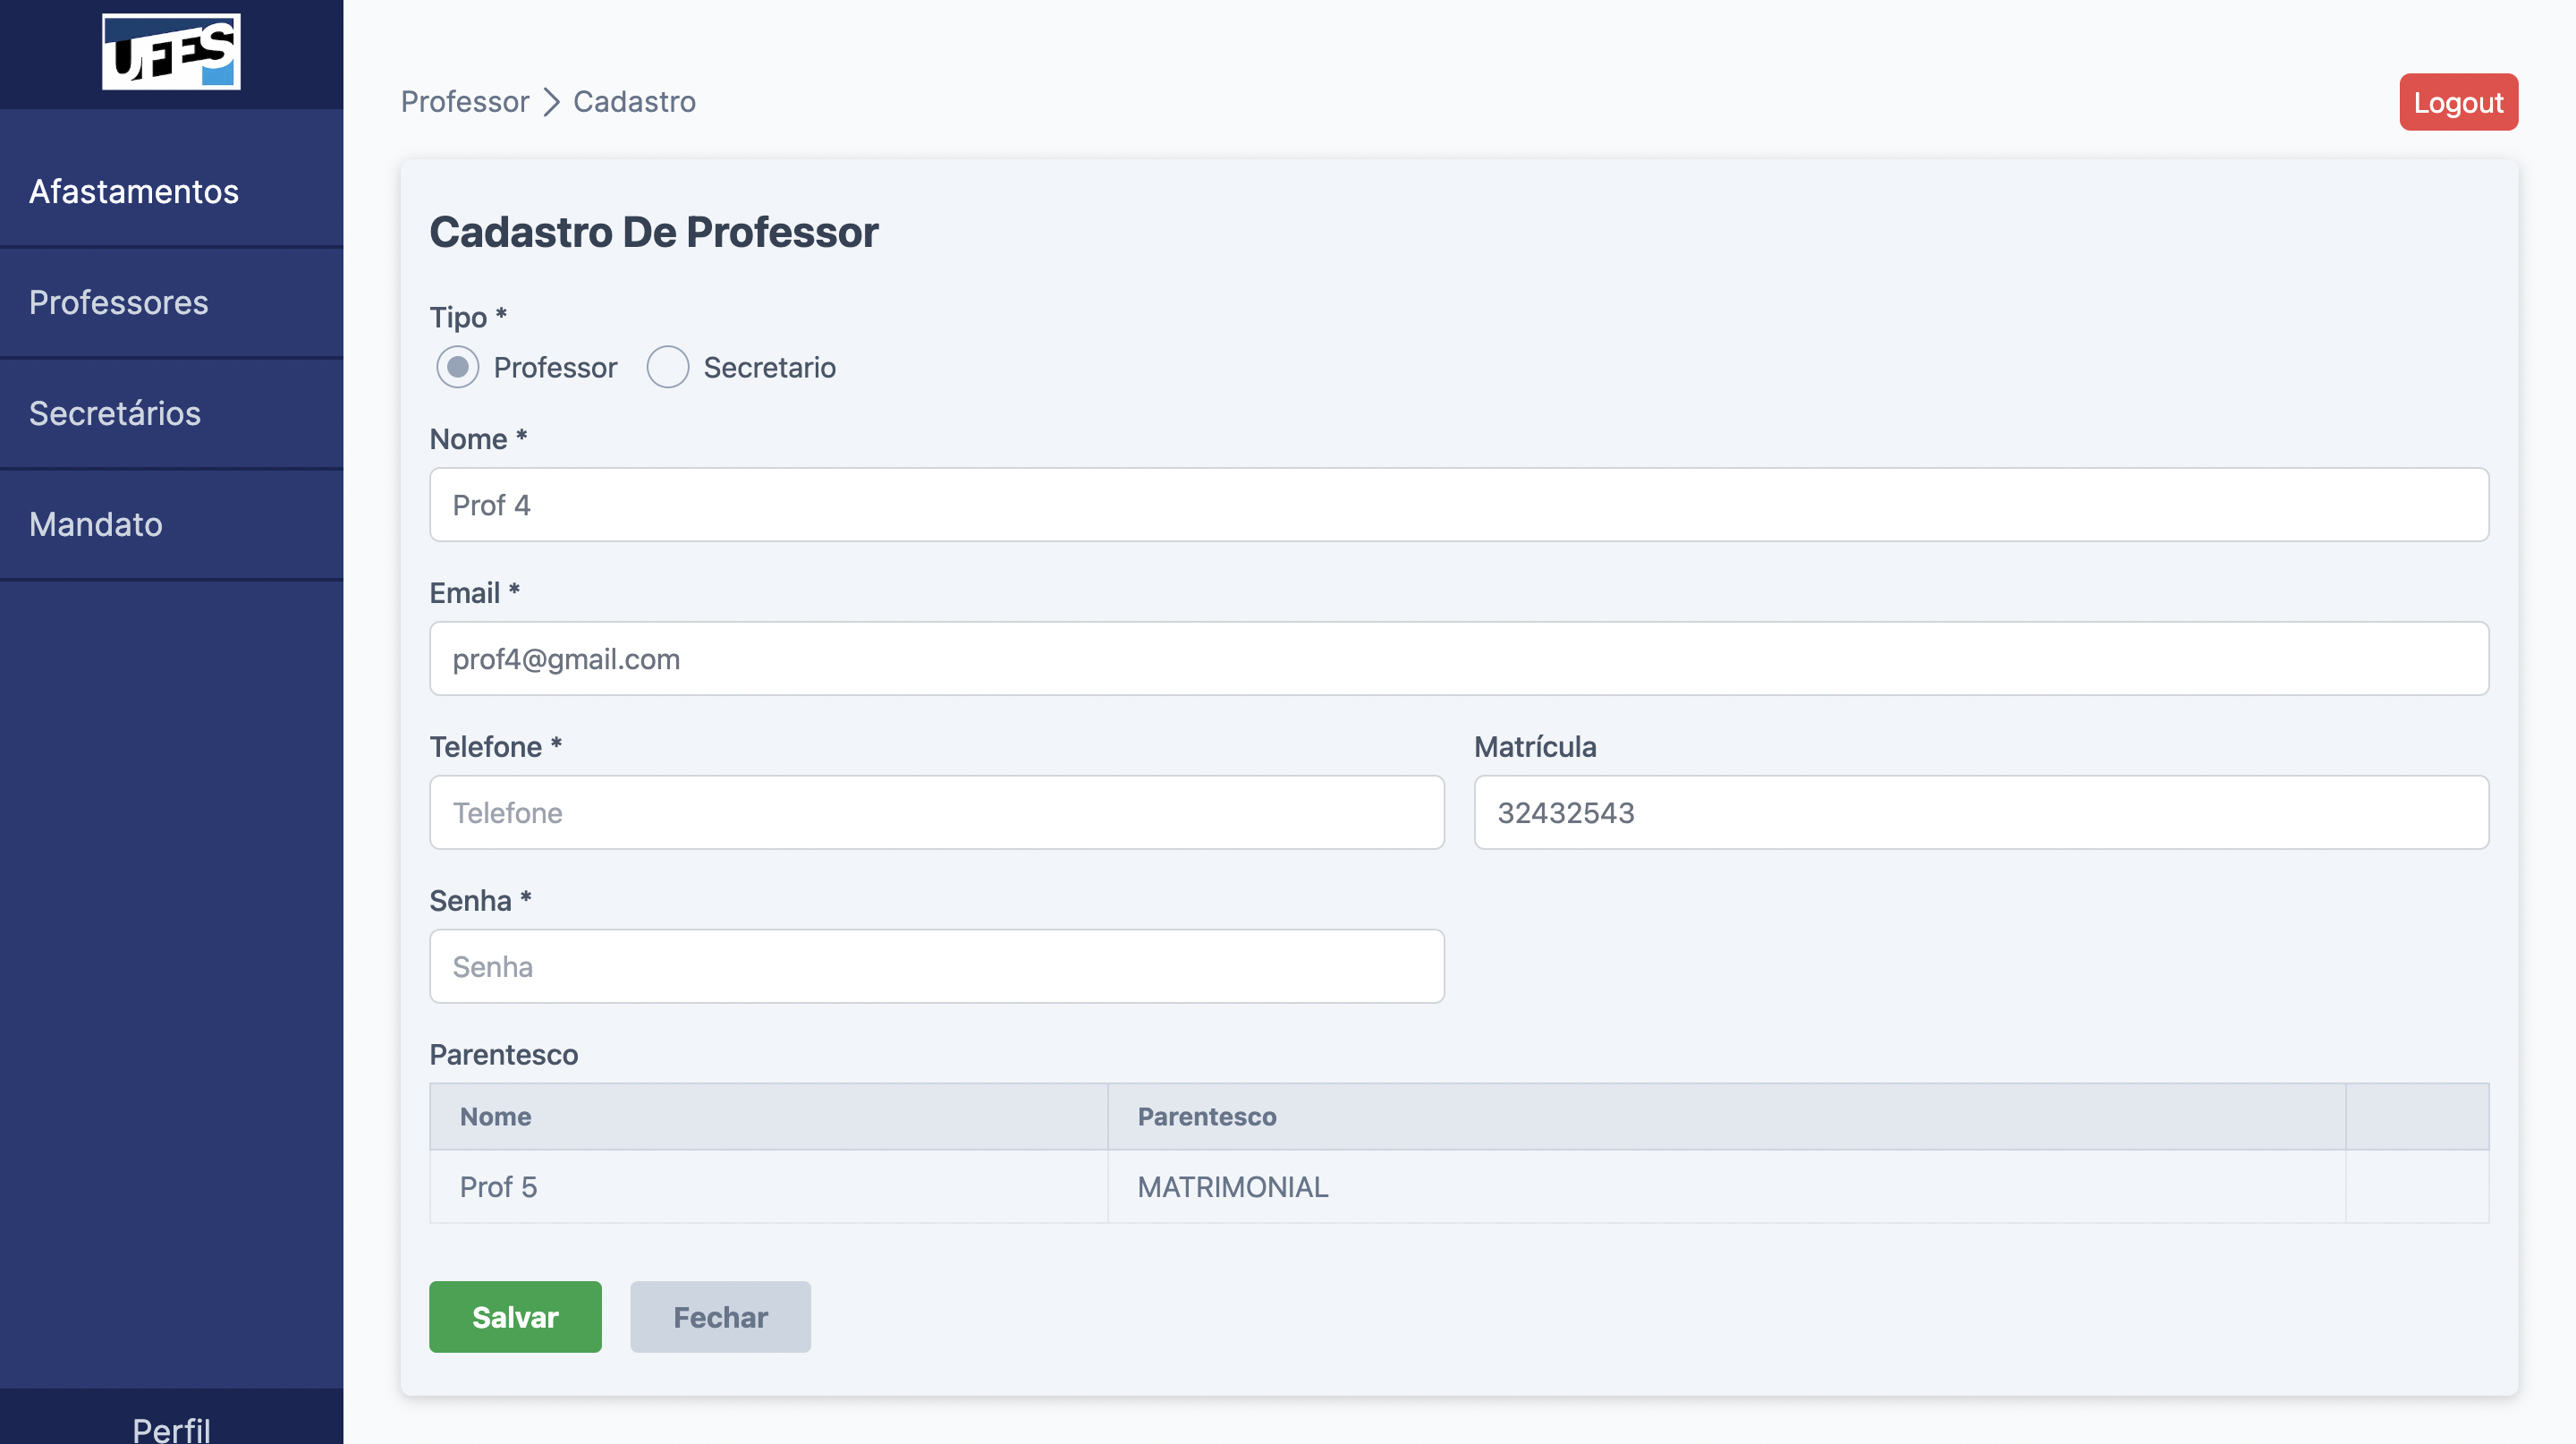
\includegraphics[width=\textwidth]{figuras/prints-app/fig-perfil.png}
    \caption{Edição de Professor do SCAP.}
    \label{fig-editar-professor}
\end{figure}


\subsection{Cadastro de Mandato}
\label{subsec-projeto-cadastro-mandato}

O secretário é responsável por gerenciar os mandatos dos professores, funções que estes exercem
no departamento. A Figura~\ref{fig-mandato} apresenta a tela de cadastro de mandatos do SCAP.
Nela é possível visualizar os mandatos atuais, e para cadastrar um novo mandato deve-se finalizar o anterior.
Para finalizar o mandato basta clicar no botão \textbf{Finalizar Mandato}, caso uma data de fim não seja enviada,
será considerada a data de hoje. Professores também podem visualizar os mandatos atuais. 

\begin{figure}[h!]
    \centering
    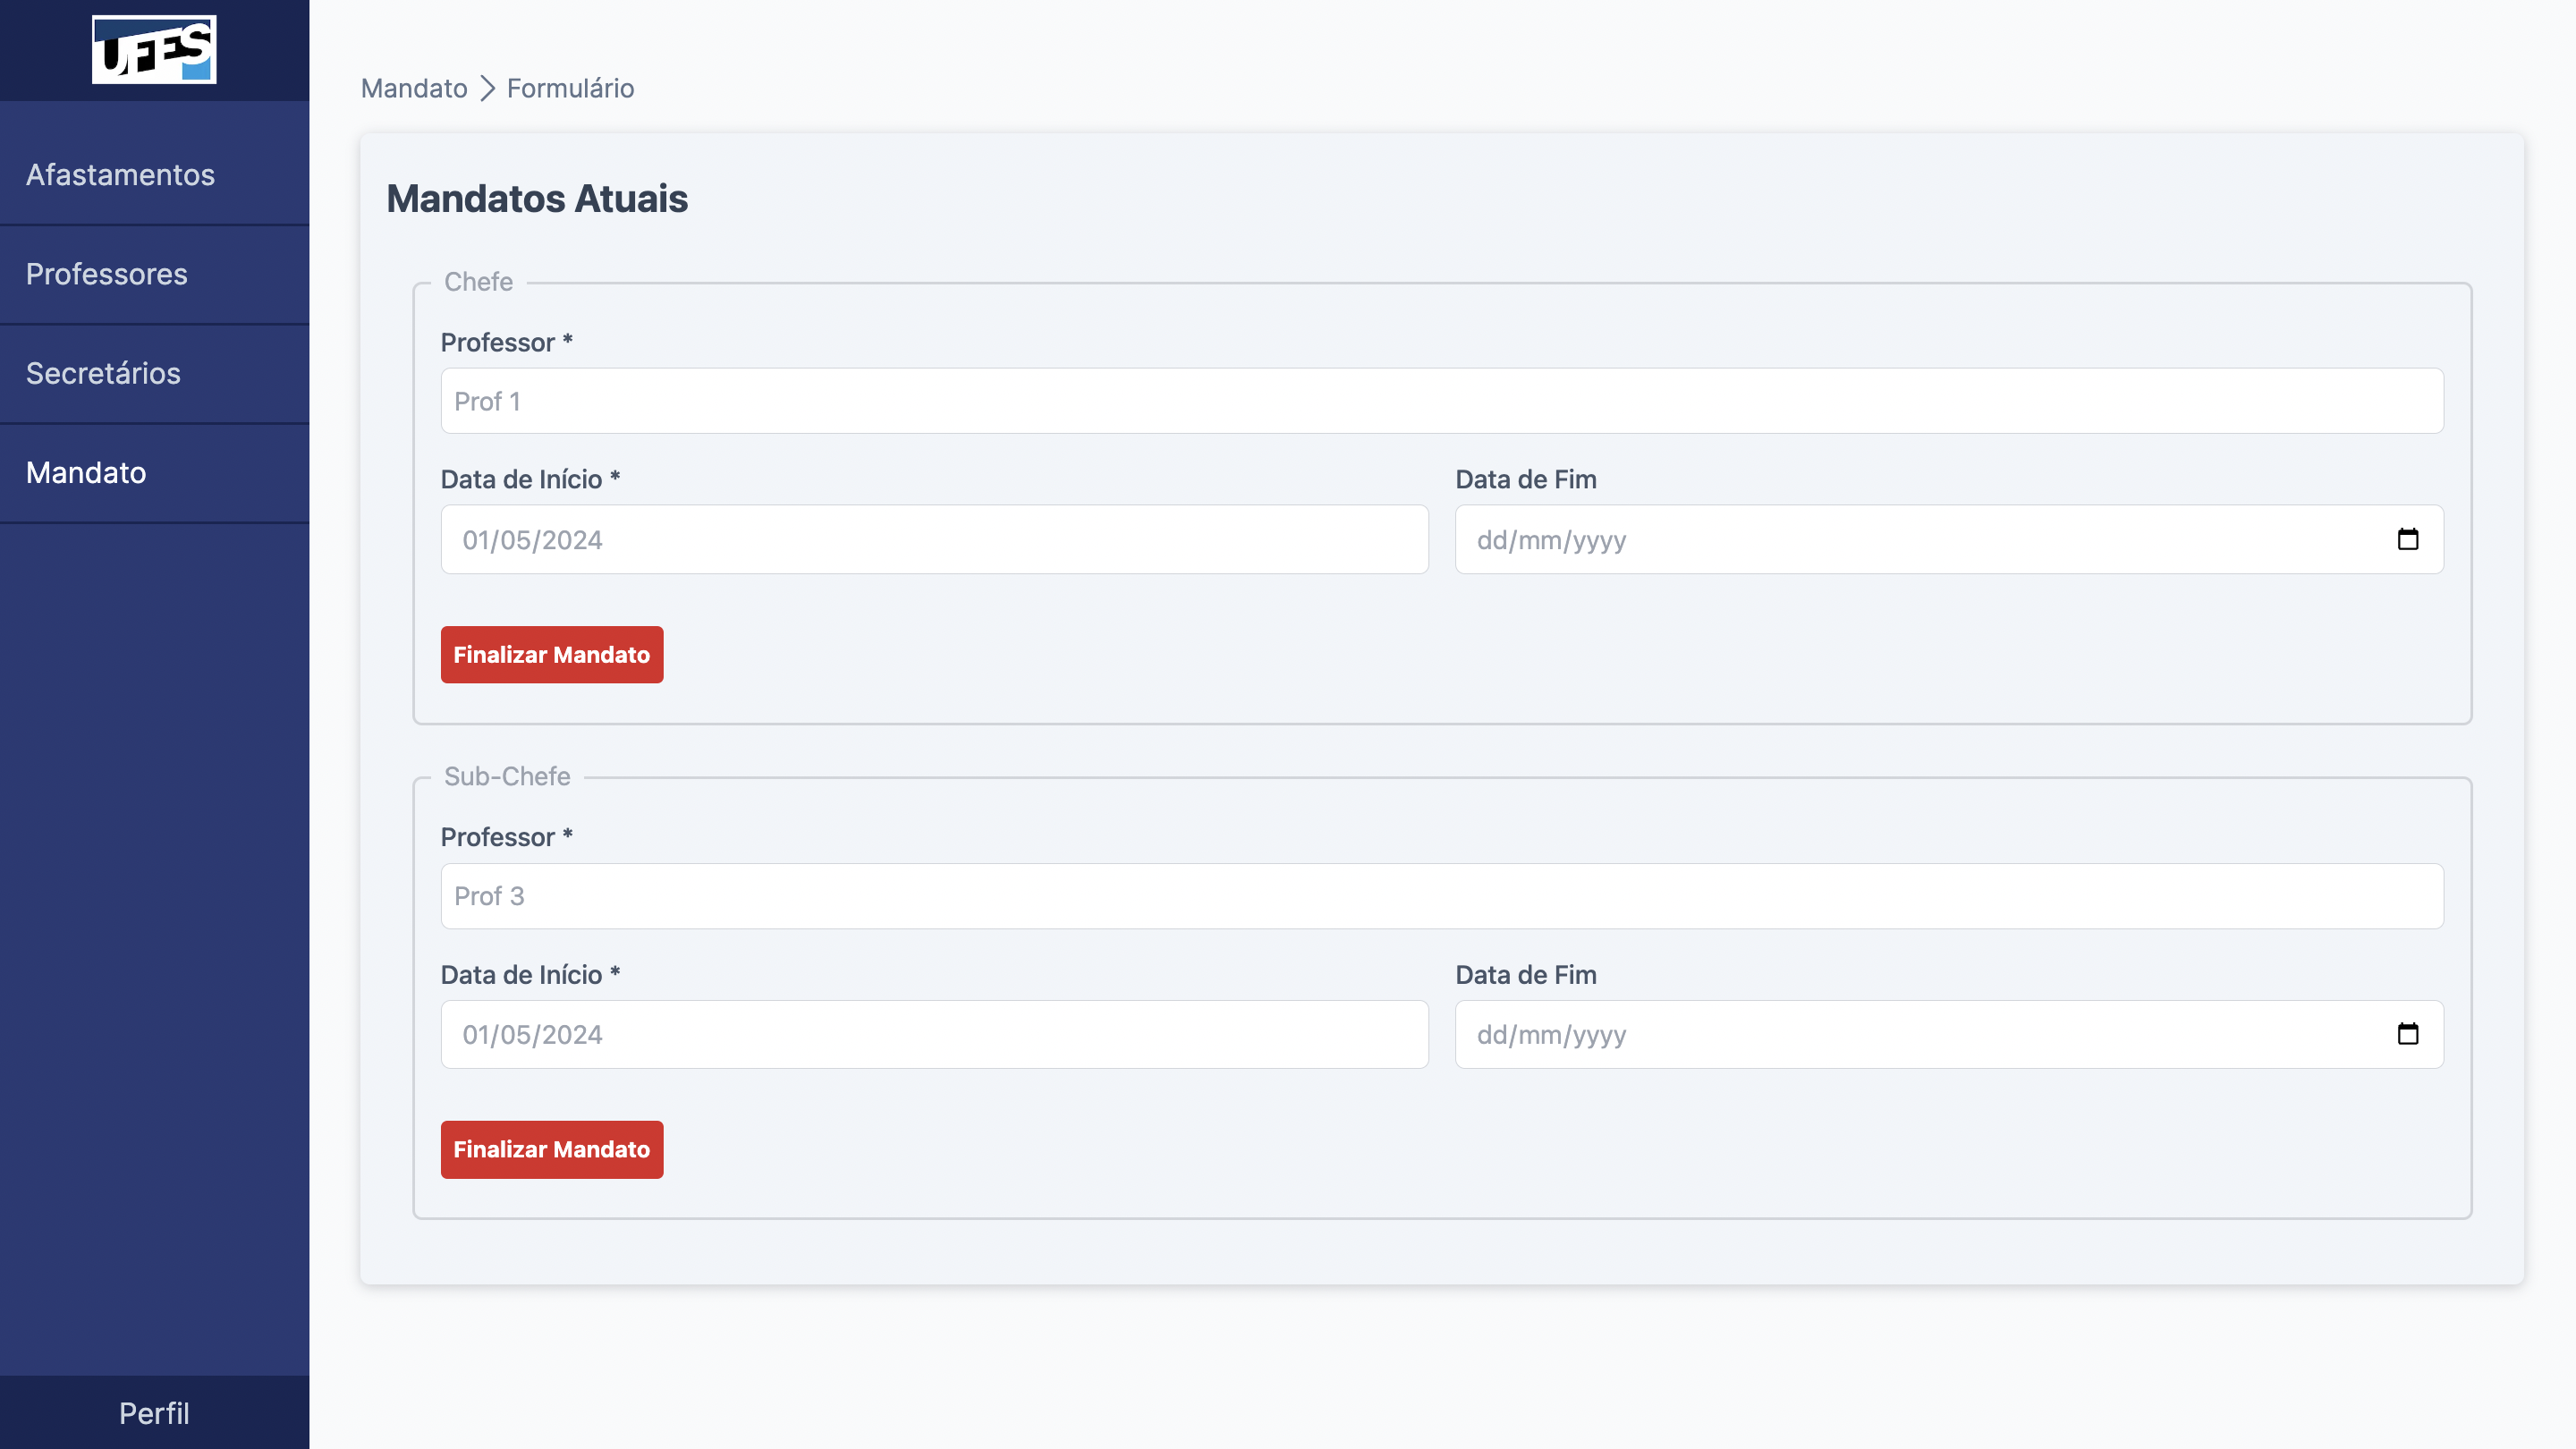
\includegraphics[width=\textwidth]{figuras/prints-app/fig-mandato-visao-secretario.png}
    \caption{Cadastro de Mandatos do SCAP.}
    \label{fig-mandato}
\end{figure}
% % ==============================================================================
% PG - Nome do Aluno
% Capítulo 5 - Considerações Finais
% ==============================================================================
\chapter{Conclusão}
\label{chap-conclusao}

% \hl{Neste capítulo devem ser realizadas as considerações finais do trabalho, sendo apresentadas suas principais contribuições, limitações, lições aprendidas durante o desenvolvimento do trabalho, dificuldades enfrentadas e perspectivas de trabalhos futuros. O capítulo deve ter entre 3 e 5 páginas.}

Este capítulo apresenta as considerações finais do trabalho, dificuldades, e perspectivas para trabalhos futuros.
Na Seção~\ref{sec-conclusoes-consideracoes}, são apresentadas as conclusões obtidas e suas relações com os objetivos definidos, enquanto
na Seção~\ref{sec-conclusoes-trabalhosfuturos} são apresentadas ideias e melhorias para trabalhos futuros.

%%% Início de seção. %%%
\section{Considerações Finais}
\label{sec-conclusoes-consideracoes}

Neste projeto uma nova implementação do SCAP aplicando o método FrameWeb foi realizada, dessa vez utilizando o \textit{framework} Next.js.
Os modelos FrameWeb produzidos foram essenciais para a implementação do SCAP, pois forneceram uma visão geral da aplicação, facilitando e agilizando o desenvolvimento do sistema.
Mesmo assim, ao longo da implementação os modelos foram revisitados diversas vezes, e inconsistências tiveram de ser consertadas.

Os objetivos definidos no Capítulo~\ref{chap-intro} estão listados abaixo.
\begin{itemize}
    \item Compreender o método FrameWeb;
    \item Analisar os requisitos da aplicação SCAP;
    \item Implementar a aplicação SCAP utilizando o \textit{framework} Next.js e o método FrameWeb.
\end{itemize}

Foi possível estudar e compreender o método FrameWeb para aplicá-lo na implementação do SCAP, considerando os requisitos levantados anteriormente.
Com isso, as disciplinas de Engenharia de Software foram revisitadas e colocadas em prática, e o conhecimento adquirido foi essencial para o andamento deste projeto.
Além disso, o projeto permitiu o aprendizado de um novo e moderno \textit{framework} de desenvolvimento, o Next.js, por meio da implementação do sistema SCAP.
Assim, os objetivos foram totalmente satisfeitos.

\vitor{Dizer explicitamente acima se os objetivos do projeto foram satisfeitos completamente, parcialmente ou não foram satisfeitos.}


% Limitações
Em seu trabalho, \citeonline{hoppe:2023} fez adaptações do modelo FrameWeb para \textit{frameworks} SPA, o que facilitou 
a modelagem dos diagramas de navegação, principalmente. No entanto, algumas dificuldades apareceram ao longo da implementação,
isso pois foram encontradas poucas referências de projetos utilizando padrões, como \textit{Repository Pattern} ou DAO, com o \textit{framework} Next.js.
Em sua maioria o Next.js é utilizado apenas como \textit{frontend}, no entanto neste projeto ele foi utilizado como \textit{fullstack}.


Tendo em vista que o foco do projeto era a aplicação e análise do método FrameWeb, duas funcionalidades não foram implementadas,
sendo elas: o envio de \textit{e-mails} e a geração de atas. Ambas funcionalidades são complexas e demandariam um tempo maior para serem implementadas.

\vitor{O trabalho do Pedro~\cite{hoppe:2023}, que você inclusive cita na Seção~\ref{sec-fundteo-frameweb}, visa trazer os frameworks SPA para o FrameWeb. O parágrafo acima não menciona isso. Elaborar melhor essa parte.}

\sophie{
Fiquei em dúvida de como escrever essa parte, acho que seria mais uma dificuldade minha do que limitação do modelo, a minha dificuldade foi em relação
a eu não conhecer o Next e não ter achado muitas referencias de padrões de projeto usando ele como fullstack
(E eu não tinha muitas experiência implementando um back assim).

O trabalho do~\cite{hoppe:2023} me pareceu ter sido mais voltado para os modelos de navegação e nos frameworks SPA
usando orientação à objeto. No meu caso os components são na verdade funções e apesar de terem também um comportamento de Controller
ainda existe um controller no back-end,
revisando os meus modelos de navegação acho até que eles podem estar errados, já que por ser função não há uma chamada de método,
mas sim chamadas à api.
}


Apesar do método FrameWeb utilizar UML, o que facilitaria a modelagem dos diagramas, a ferramenta utilizada para a modelagem, o \textit{Visual Paradigm}, 
tem uma curva de aprendizado acentuada, o que inicialmente dificultou a modelagem dos diagramas. Além disso, a ferramenta possui suporte para a geração de código
a partir dos diagramas, porém houve uma grande dificuldade de usá-la, o que fez com que a implementação fosse feita manualmente.

\vitor{A ferramenta possui suporte pra geração de código de alguns modelos (falta o de Navegação), mas para gerar código para o framework que você escolheu, é preciso construir os templates. Acertar o parágrafo acima para explicar de forma mais precisa porque não foi usada a geração de código.}
\sophie{Implementei os templates mas não consegui gerar, achei que a documentação não estava completamente clara.
Posso escrever isso e dizer que um trabalho futuro seria melhorar a ferramenta e documentação?}


%%% Início de seção. %%%
\section{Trabalhos Futuros}
\label{sec-conclusoes-trabalhosfuturos}

% \hl{Nesta seção devem ser identificados trabalhos futuros que poderão ser realizados a partir dos resultados obtidos até o momento no trabalho. Idealmente, trabalhos futuros não devem apenas ser citados. Recomenda-se discutir aspectos sobre como podem ser realizados e por que é importante que sejam realizados (que benefícios podem ser obtidos com sua realização).}

Para trabalhos futuros, seria interessante analisar se os requisitos de fato contemplam as necessidades do departamento,
implementar as funcionalidades que ficaram pendentes, e fazer o \textit{deploy} da aplicação em um servidor.

Além disso, seria também interessante utilizar as ferramentas de modelagem, sejam elas o Editor FrameWeb~\cite{campos:2017} ou o \textit{Visual Paradigm} com o plugin desenvolvido~\cite{silva:2023},
com aplicações utilizando JavaScript, assim como testar o gerador de código.

A grande maioria das aplicações, dos trabalhos anteriores, apresentados na Tabela~\ref*{tbl-comparacao-trabalhos}, foram feitas utilizando \textit{frameworks} Java, JavaScript ou PHP. Portanto, para ampliar
o campo da pesquisa, seria interessante
implementar o sistema também com \textit{frameworks} Python,\footnote{Python, \url{https://www.python.org}} como Django, ou com \textit{frameworks} Ruby,\footnote{Ruby, \url{https://www.ruby-lang.org/en/}} como Ruby on Rails,
linguagens essas muito utilizados no mercado atual.
Por fim, para deixar o modelo mais robusto, é importante comparar todos os resultados obtidos ao longo de todas as diferentes implementações feitas.

\vitor{Acho que você poderia incluir aqui a tabela com os trabalhos anteriores que implementaram o SCAP, pegando o que o Danillo Gomes fez na Tabela 2 do TCC dele e atualizando com o seu trabalho. Isso mostraria que faltam implementações com Python e Ruby, como você diz no parágrafo. Você pode obter o código-fonte \LaTeX\ da tabela aqui: \url{https://bitbucket.org/vitorsouza-students/pg-2022-danilo-gomes/src/main/pg-monografia/capitulos/ch4-avaliacao.tex}. O TCC do Danillo em PDF está aqui: \url{http://www.inf.ufes.br/~vitorsouza/wp-content/papercite-data/pdf/gomes-pg22.pdf}}


\begin{table}[h]
	\caption{Listagem de implementações do SCAP.}
	\label{tbl-comparacao-trabalhos}
	\centering\def\tabularxcolumn#1{m{#1}}\def\arraystretch{1.0}
	\begin{tabularx}{\textwidth}{ 
			| >{\hsize=0.4\hsize}X
			| >{\hsize=0.5\hsize}X	
			| >{\hsize=0.7\hsize}X
			| >{\hsize=0.4\hsize}X
			|
		}
		\hline
		\textbf{Trabalho} & 
		\textbf{\textit{Framework} MVC} & 
		\textbf{Tecnologia ORM} &
		\textbf{Tecnologia DI} \\
		\hline
		
		\citeonline{duarte:2014} &
		JSF (Java) & 
		Hibernate (Data Mapper) &
		CDI \\ 
		\hline 
		
		\citeonline{prado:2015} & 
		VRaptor (Java) & 
		Hibernate (Data Mapper) &
		CDI \\
		\hline 
		
		\citeonline{pinheiro:2017} & 
		Laravel (PHP) &
		Eloquent (Active Record)  &
		Não utilizou \\
		\hline
		
		\citeonline{matos:2017} & 
		Spring (Java) &
		Hibernate (Data Mapper)  &
		Embutido no Spring \\
		\hline 
		
		\citeonline{matos:2017} & 
		Vaadin (Java) &
		Hibernate (Data Mapper)  &
		Não utilizou \\
		\hline 
		
		\citeonline{avelar:2018} & 
		Ninja (Java) &
		Hibernate (Data Mapper)  &
		Google Guice \\
		\hline 
		
		\citeonline{ferreira:2018} & 
		Wicket (Java) &
		Hibernate (Data Mapper)  &
		CDI \\ 
		\hline 
		
		\citeonline{ferreira:2018} & 
		Tapestry (Java) &
		Hibernate (Data Mapper)  &
		Embutido no Tapestry \\ 
		\hline 
		
		\citeonline{meirelles:2019} & 
		CodeIgniter (PHP) &
		Embutido no CodeIgniter (Active Record) &
		Não utilizou \\
		\hline 
		
		\citeonline{meirelles:2019} & 
		NodeJS (JavaScript) &
		Não utilizou  &
		Não utilizou \\ 
		\hline 
		
		\citeonline{guterres:2019} & 
		Play (Scala) &
		Slick (Padrão não identificado)  &
		Não utilizou \\ 
		\hline 
		
     	\citeonline{dalapicola:2021} & 
		AdonisJS e Quasar (Javascript) &
		Lucid (Active Record)  &
		Embutido no AdonisJS \\ 
		\hline 
		
		\citeonline{berger:2021} & 
		Yii (PHP) &
		Yii  (Data Mapper)  &
		Embutido no Yii \\ 
		\hline 
		
		\citeonline{berger:2021} & 
		Symfony (PHP)  &
		Doctrine (Active Record)  &
		Embutido no Symfony \\ 
		\hline 
	
	    \citeonline{gomes:2022} & 
		Angular e NodeJS(JavaScript) &
		TypeORM (Data Mapper)  &
		Embutido no Angular\\ 
		\hline 

        Este &
        Next.js (TypeScript) &
        Prisma (Data Mapper) &
        Não utilizou \\
        \hline
		
	\end{tabularx}
\end{table}

% % ==============================================================================
% PG - Nome do Aluno
% Capítulo 6 - Dicas LaTeX
% ==============================================================================
\chapter{Dicas para escrita em \latex}
\label{sec-dicaslatex}

Utilizaremos este capítulo para apresentar alguns exemplos de uso de \latex que podem ser úteis para aqueles que possuem pouca experiência com a ferramenta e vão escrever a monografia usando \latex. Para mais informações sobre \latex, você pode consultar a  \href{https://www.overleaf.com/learn}{documentação do overleaf} ou vários materiais disponíveis online, como  \href{https://www.ime.usp.br/~viviane/MAP2212/minicurso.pdf}{esse minicurso da USP}.

Este capítulo deve ser excluído da monografia. Sugere-se também excluir as figuras e listagens usadas aqui como exemplo.



%%% Início de seção. %%%
\section{Seções e subseções}
\label{sec-dicaslatex-secoes}

O documento é organizado em capítulos (\texttt{\textbackslash chapter\{\}}), seções (\texttt{\textbackslash section\{\}}), subseções (\texttt{\textbackslash subsection\{\}}), sub-subseções (\texttt{\textbackslash subsubsection\{\}}) e assim por diante. Atenção, porém, a não criar estruturas muito profundas (sub-sub-sub-...) pois o documento não fica bem estruturado.


%%% Início de seção. %%%
\subsection{Referências a seções}
\label{sec-dicaslatex-secoes-refs}

Cada parte do documento (capítulo, seção, etc.) deve possuir um rótulo logo abaixo de sua definição. Por exemplo, este capítulo é definido com \texttt{\textbackslash chapter\{Introdução\}} seguido por \texttt{\textbackslash label\{sec-dicaslatex\}}. Assim, podemos fazer referências cruzadas usando o comando \texttt{\textbackslash ref\{rótulo\}}: ``O Capítulo~\ref{sec-dicaslatex} começa com a Seção~\ref{sec-dicaslatex-secoes}, que é ainda subdividida nas subseções~\ref{sec-dicaslatex-secoes-refs} e~\ref{sec-dicaslatex-secoes-sobrerefs}.

Para melhor organização das partes do documento, sugere-se primeiro utilizar o prefixo \texttt{sec-} (para diferenciar de referências à figuras, tabelas, etc. quando usarmos o comando \texttt{\textbackslash ref\{\}}) e também representar a hierarquia das seções nos rótulos. Por exemplo, o Capítulo~\ref{sec-dicaslatex} tem rótulo \texttt{sec-dicaslatex}, sua Seção~\ref{sec-dicaslatex-secoes} tem rótulo \texttt{sec-dicaslatex-secoes} e a Subseção~\ref{sec-dicaslatex-secoes-refs} tem rótulo \texttt{sec-dicaslatex-secoes-refs}.



%%% Início de seção. %%%
\subsection{Sobre referências cruzadas}
\label{sec-dicaslatex-secoes-sobrerefs}

Nas próximas seções, veremos que é possível fazer referência cruzada não só a seções mas também a listagens de código, figuras, tabelas, etc. Em todos estes casos, quando nos referimos à Seção X, Listagem Y ou Figura Z, consideramos que estes são os nomes próprios destes elementos e, portanto, usa-se a primeira letra maiúscula. Isso pode ser visto na Subseção~\ref{sec-dicaslatex-secoes-refs}, acima. A exceção é quando nos referimos a vários elementos ao mesmo tempo, por exemplo: ``as subseções~\ref{sec-dicaslatex-secoes-refs} e~\ref{sec-dicaslatex-secoes-sobrerefs}''.

Por fim, ao usar o comando \texttt{\textbackslash ref\{\}}, sugere-se separá-lo da palavra que vem antes dele com um \textasciitilde\ ao invés de espaço. Por exemplo: \texttt{o capítulo\textasciitilde \textbackslash ref\{sec-dicaslatex\}}. Isso faz com que o \latex não quebre linha entre a palavra \texttt{capítulo} e o número do capítulo.




%%% Início de seção. %%%
\section{Citações bibliográficas}
\label{sec-dicaslatex-citacoes}

Este documento utiliza a ferramenta de gerenciamento de referências bibliográficas do \latex, chamada \emph{BibTeX}. O arquivo \texttt{bibliografia.bib}, referenciado no arquivo \latex principal deste documento, contém algumas referências bibliográficas de exemplo. Assim como capítulos, seções, etc., tais referências também possuem rótulos, especificados como primeiro parâmetro de cada entrada (ex.: \texttt{@incollection\{souza-et-al:iism08, ...\}}.

Sugere-se um padrão para rótulos de referências bibliográficas para que fique claro também no código \latex qual referência está sendo citada. Por exemplo, ao citar a referência \texttt{souza-et-al:sesas13}, sabemos que é um artigo escrito por \emph{Souza} e outros, publicado no \emph{SESAS} em \emph{2013} (geralmente a pessoa que citou sabe que publicação é SESAS e quem é Souza).

Para citar uma referência bibliográfica contida no arquivo \emph{BibTeX}, basta usar seu rótulo como parâmetro de um de dois comandos possíveis de citação:

\begin{itemize}
	\item O comando \texttt{\textbackslash cite\{\}} efetua uma citação tradicional, colocando o nome do(s) autor(es) e o ano entre parênteses. Por exemplo, \texttt{\textbackslash cite\{souza-et-al:iism08\}} é transformado em \cite{souza-et-al:iism08};
	
	\item O comando \texttt{\textbackslash citeonline\{\}} efetua uma citação integrada ao texto, colocando o nome do(s) autor(es) direto no texto e somente o ano entre parênteses. Por exemplo, ``de acordo com \texttt{\textbackslash citeonline\{souza-et-al:iism08\}}'' é transformado em: de acordo com \citeonline{souza-et-al:iism08};
\end{itemize}

Também é possível citar vários trabalhos de uma só vez, separando os rótulos das referências bibliográficas com uma vírgula dentro do comando apropriado. Por exemplo, \texttt{\textbackslash cite\{souza-et-al:sesas13,souza-et-al:csrd13\}} \cite{souza-et-al:sesas13,souza-et-al:csrd13}.

Os trabalhos citados são automaticamente incluídos na seção de referências bibliográficas, ao final do documento. Tudo é formatado automaticamente segundo padrões da ABNT.



%%% Início de seção. %%%
\section{Listagens de código}
\label{sec-dicaslatex-listagens}

O pacote \texttt{listings}, incluído neste template, permite a inclusão de listagens de código. Análogo ao já feito anteriormente, listagens possuem rótulos para que possam ser referenciadas e sugerimos uma regra de nomenclatura para tais rótulos: usar como prefixo o rótulo do capítulo, substituindo \texttt{sec-} por \texttt{lst-}.

A Listagem~\ref{lst-intro-exemplo}, por exemplo, possui o rótulo \texttt{lst-intro-exemplo} e representa o código que foi usado no próprio documento para exibir as listagens desta seção. Como podemos ver, a sugestão é que os arquivos de código sejam colocados dentro da pasta \texttt{codigos/} e tenham nome idêntico ao rótulo, colocando a extensão adequada ao tipo de código.

\lstinputlisting[label=lst-intro-exemplo, caption=Exemplo de código \latex para inclusão de listagens de código., float=htpb]{codigos/lst-intro-exemplo.tex}

A Listagem~\ref{lst-intro-outroexemplo} mostra um exemplo de listagem com especificação da linguagem utilizada no código. O pacote \texttt{listings} reconhece algumas linguagens\footnote{Veja a lista de linguagens suportadas em \url{http://en.wikibooks.org/wiki/LaTeX/Source\_Code\_Listings\#Supported_languages}.} e faz ``coloração'' de código (na verdade, usa \textbf{negrito} e não cores) de acordo com a linguagem. O parâmetro \texttt{float=htpb} incluído em ambos os exemplos impede que a listagem seja quebrada em diferentes páginas.

\lstinputlisting[label=lst-intro-outroexemplo, caption=Exemplo de código \java especificando linguagem utilizada., language=Java, float=htpb]{codigos/lst-intro-outroexemplo.java}



%%% Início de seção. %%%
\section{Figuras}
\label{sec-dicaslatex-figuras}

Figuras podem ser inseridas no documento usando o \emph{ambiente} \texttt{figure} (ou seja, \texttt{\textbackslash begin\{figure\}} e \texttt{\textbackslash end\{figure\}}) e o comando \texttt{\textbackslash includegraphics\{\}}. Existem alguns outros elementos e propriedades úteis de serem configuradas, resultando no código exibido na Listagem~\ref{lst-intro-figuras}.

\lstinputlisting[label=lst-intro-figuras, caption=Código \latex utilizado para inclusão das figuras na Seção~\ref{sec-dicaslatex-figuras}., float=htpb]{codigos/lst-intro-figuras.tex}

O comando \texttt{\textbackslash centering} centraliza a figura na página. A opção \texttt{width} do comando \texttt{\textbackslash includegraphics\{\}} determina o tamanho da figura e usa-se \texttt{\textbackslash textwidth} (opcionalmente multiplicado por um número) para se referir à largura da página.

O parâmetro do comando \texttt{\textbackslash includegraphics\{\}} indica onde a imagem pode ser encontrada. Foi criado o diretório \texttt{figuras/} para conter as figuras do documento, dando uma melhor organização aos arquivos. Ao abrir esta pasta, repare que as figuras possuem duas versões---uma em \texttt{.eps} e outra em \texttt{.pdf}---e que o comando \texttt{\textbackslash includegraphics\{\}} não especifica a extensão. Isso se dá porque o \latex possui um compilador para formato PostScript (\texttt{latex}) que espera as imagens em \texttt{.eps} e um compilador para PDF (\texttt{pdflatex}) que espera as imagens em \texttt{.pdf}. Dependendo do seu ambiente \latex, é possível apenas colocar as figuras em formatos mais comuns, como JPG ou PNG e ele incluir no PDF sem problemas. Vale a pena testar.

Por fim, o comando \texttt{\textbackslash caption\{\}} especifica a descrição da figura e \texttt{\textbackslash label\{\}}, como de costume, estabelece um rótulo para permitir referência cruzada de figuras. Note ainda que é utilizada a mesma estratégia de nomenclatura de rótulos usada nas listagens, porém utilizando o prefixo \texttt{fig-}.

As figuras~\ref{fig-intro-exemplo} e~\ref{fig-intro-exemplosideways} mostram o resultado do código da Listagem~\ref{lst-intro-figuras}. A Figura~\ref{fig-intro-exemplosideways}, em particular, utiliza o pacote \texttt{rotating} para mostrar figuras largas em modo paisagem. Basta usar o ambiente \texttt{sidewaysfigure} ao invés de \texttt{figure}.

\begin{figure}
	\centering
	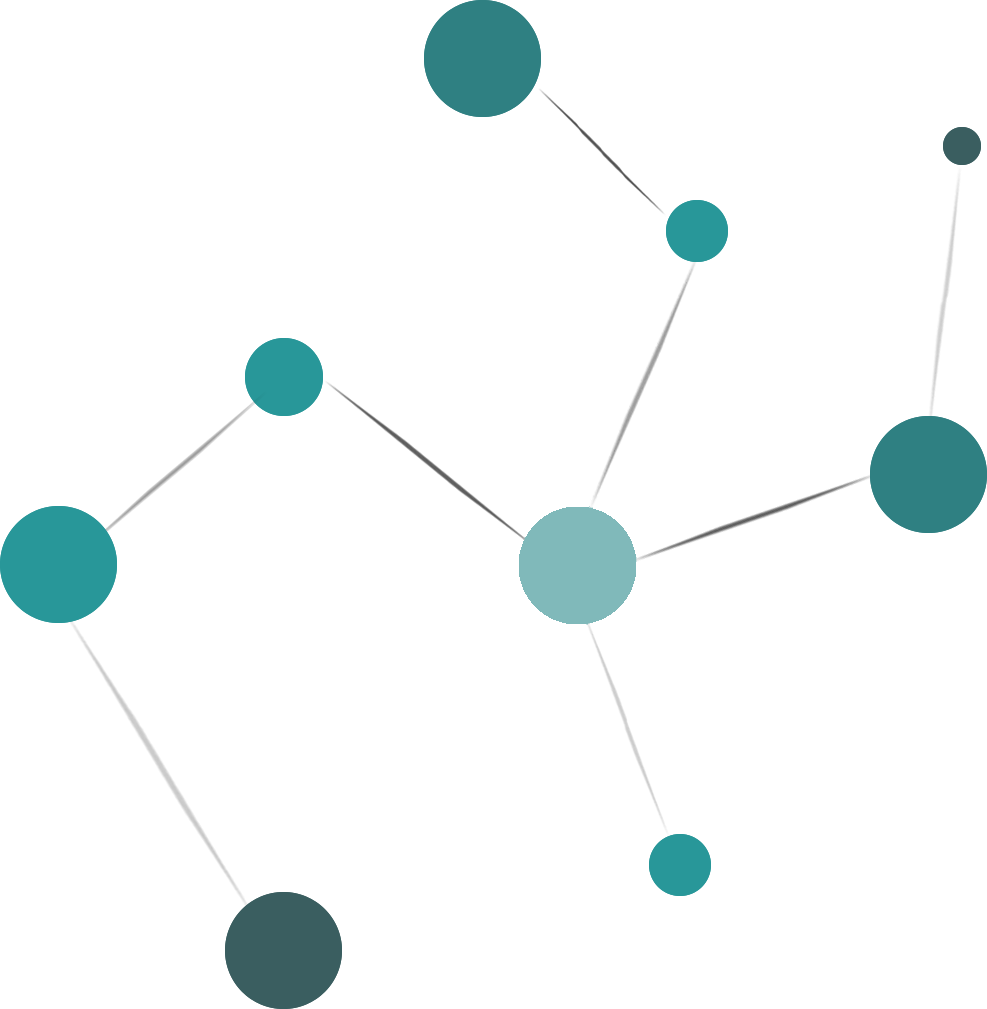
\includegraphics[width=.25\textwidth]{figuras/image-home.png} 
	\caption{Exemplo de figura.}
	\label{fig-intro-exemplo}
\end{figure}

\begin{sidewaysfigure}
	\centering
	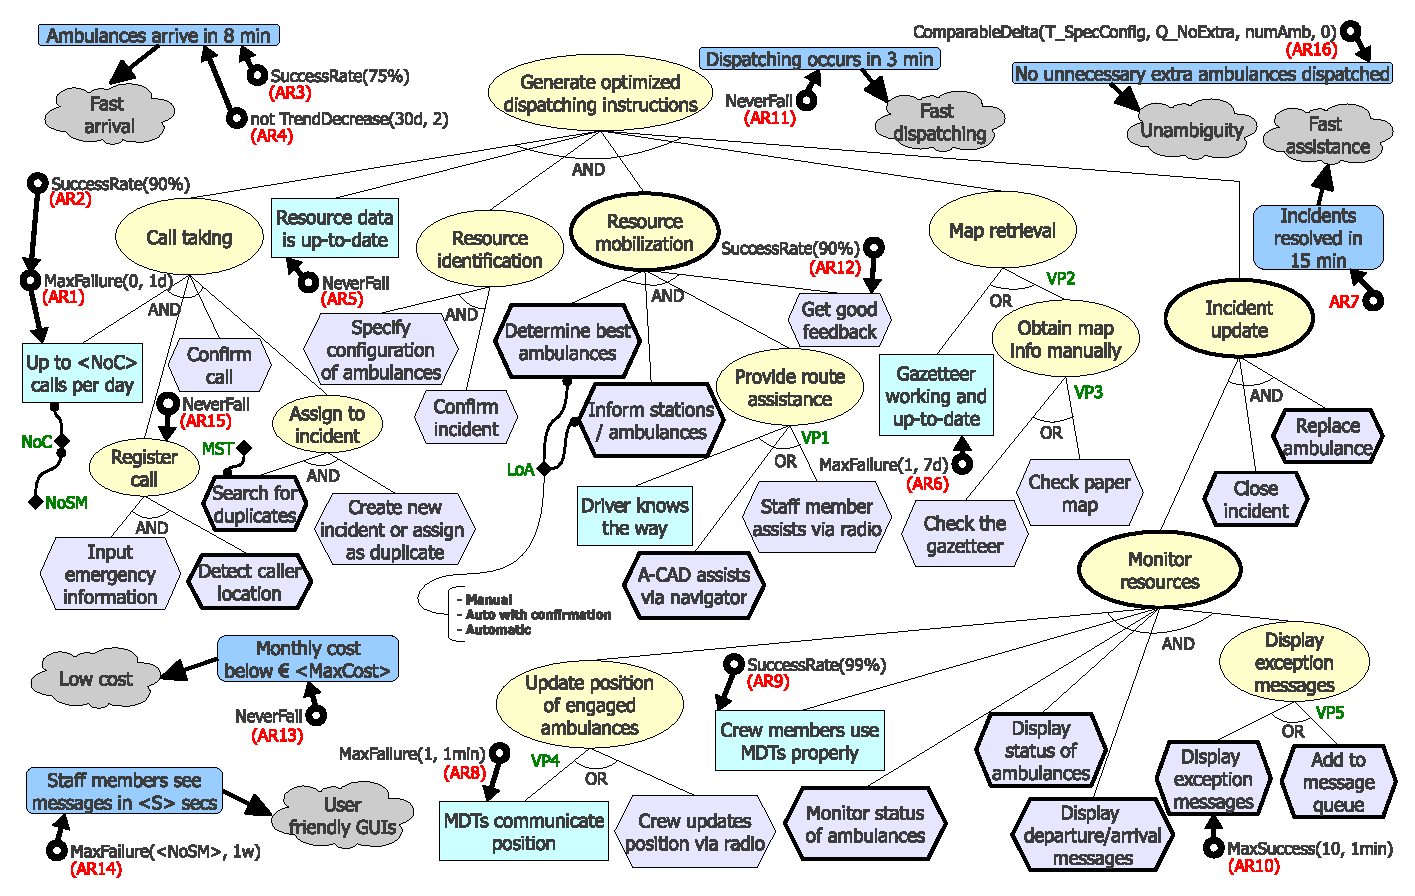
\includegraphics[width=\textwidth]{figuras/fig-intro-exemplosideways} 
	\caption{Exemplo de figura em modo paisagem: um modelo de objetivos~\cite{souza-mylopoulos:spe13}.}
	\label{fig-intro-exemplosideways}
\end{sidewaysfigure}



%%% Início de seção. %%%
\section{Tabelas}
\label{sec-dicaslatex-tabelas}

Tabelas são um ponto fraco do \latex. Elas são complicadas de fazer e, dependendo da complexidade da tabela (muitas células mescladas, por exemplo), vale a pena construi-las em outro programa (por exemplo, em seu editor de texto favorito) e inclui-las no documento como figuras. Mostramos, no entanto, alguns exemplos de tabela a seguir. O código utilizado para criar as tabelas encontra-se nas listagens~\ref{lst-intro-tabelas01}, \ref{lst-intro-tabelas02} e~\ref{lst-intro-tabelas03}.

\lstinputlisting[label=lst-intro-tabelas01, caption=Código \latex utilizado para inclusão das tabelas~\ref{tbl-intro-exemplo01} e~\ref{tbl-intro-exemplo02}., float=htpb]{codigos/lst-intro-tabelas01.tex}

\lstinputlisting[label=lst-intro-tabelas02, caption=Código \latex utilizado para inclusão da Tabela~\ref{tbl-intro-exemplo03}., float=htpb]{codigos/lst-intro-tabelas02.tex}

\lstinputlisting[label=lst-intro-tabelas03, caption=Código \latex utilizado para inclusão da Tabela~\ref{tbl-intro-exemplo04}., float=htpb]{codigos/lst-intro-tabelas03.tex}

Em particular, a Tabela~\ref{tbl-intro-exemplo04} utiliza um pacote chamado \texttt{tabularx}, que permite maior controle do layout das tabelas. Ao definir o ambiente \texttt{\textbackslash begin\{tabularx\}}, são definidos os tamanhos de cada coluna proporcional à largura ocupada pela tabela. Veja na Listagem~\ref{lst-intro-tabelas03} que as primeiras duas colunas não definem o atributo \texttt{\textbackslash hsize}, o que faz com que elas fiquem com o tamanho padrão de coluna, que é a largura da tabela dividida pelo número de colunas. Já a terceira coluna define \texttt{\textbackslash hsize=1.2\textbackslash hsize}, ou seja, esta coluna deve ser 20\% maior do que o tamanho padrão. Para isso, é preciso retirar de outras colunas, portanto a quarta e quinta colunas são definidas como 10\% menores (ou seja, \texttt{\textbackslash hsize=0.9\textbackslash hsize}).

% Exemplo de tabela 01:
\begin{table}
	\caption{Exemplo de tabela com diferentes alinhamentos de conteúdo.}
	\label{tbl-intro-exemplo01}
	\centering
	\begin{tabular}{ | c | l | r | p{40mm} |}\hline
		\textbf{Centralizado} & \textbf{Esquerda} & \textbf{Direita} & \textbf{Parágrafo}\\\hline
		C & L & R & Alinhamento de tipo parágrafo especifica largura da coluna e quebra o texto automaticamente.\\
		\hline
		Linha 2 & Linha 2 & Linha 2 & Linha 2\\
		\hline
	\end{tabular}
\end{table}

% Exemplo de tabela 02:
\begin{table}
	\caption{Exemplo que especifica largura de coluna e usa lista enumerada (adaptada de~\cite{souza-mylopoulos:spe13}).}
	\label{tbl-intro-exemplo02}
	\centering
	\renewcommand{\arraystretch}{1.2}
	\begin{small}
		\begin{tabular}{ | p{15mm} | p{77mm} | p{55mm} |}\hline
			\textbf{\textit{AwReq}} & \textbf{Adaptation strategies} & \textbf{Applicability conditions}\\\hline
			
			AR1 &
			\vspace{-2mm}\begin{enumerate}[topsep=0cm, partopsep=0cm, itemsep=0cm, parsep=0cm, leftmargin=0.5cm]
				\item \textit{Warning(``AS Management'')}
				\item \textit{Reconfigure($\varnothing$)}
			\end{enumerate}\vspace{-4mm} &
			\vspace{-2mm}\begin{enumerate}[topsep=0cm, partopsep=0cm, itemsep=0cm, parsep=0cm, leftmargin=0.5cm]
				\item Once per adaptation session;
				\item Always.
			\end{enumerate}\vspace{-4mm}
			\\\hline
			
			AR2 &
			\vspace{-2mm}\begin{enumerate}[topsep=0cm, partopsep=0cm, itemsep=0cm, parsep=0cm, leftmargin=0.5cm]
				\item \textit{Warning(``AS Management'')}
				\item \textit{Reconfigure($\varnothing$)}
			\end{enumerate}\vspace{-4mm} &
			\vspace{-2mm}\begin{enumerate}[topsep=0cm, partopsep=0cm, itemsep=0cm, parsep=0cm, leftmargin=0.5cm]
				\item Once per adaptation session;
				\item Always.
			\end{enumerate}\vspace{-4mm}
			\\\hline
		\end{tabular}
	\end{small}
\end{table}

% Exemplo de tabela 03:
\begin{table}
	\caption{Exemplo que mostra equações em duas colunas (adaptada de~\cite{souza-mylopoulos:spe13}).}
	\label{tbl-intro-exemplo03}
	\centering
	\vspace{1mm}
	\fbox{\begin{minipage}{.98\linewidth}
			\begin{minipage}{0.51\linewidth}
				\vspace{-4mm}
				\begin{eqnarray}
				\Delta \left( I_{AR1} / NoSM \right) \left[ 0, maxSM \right] > 0\\
				\Delta \left( I_{AR2} / NoSM \right) \left[ 0, maxSM \right] > 0\\
				\Delta \left( I_{AR3} / LoA \right) < 0\\
				\end{eqnarray}
				\vspace{-6mm}
			\end{minipage}
			\hspace{2mm}
			\vline 
			\begin{minipage}{0.41\linewidth}
				\vspace{-4mm}
				\begin{eqnarray}
				\Delta \left( I_{AR11} / VP2 \right) < 0\\
				\Delta \left( I_{AR12} / VP2 \right) > 0\\
				\Delta \left( I_{AR6} / VP3 \right) > 0\\
				\end{eqnarray}
				\vspace{-6mm}
			\end{minipage}
	\end{minipage}}
\end{table}

% Exemplo de tabela 04:
\begin{table}[h]
	\caption{Exemplo que utiliza o pacote \texttt{tabularx}, extraído de um artigo ainda não publicado.}
	\label{tbl-intro-exemplo04}
	\centering\tiny\def\tabularxcolumn#1{m{#1}}
	\begin{tabularx}{\columnwidth}{ >{\centering}X | >{\centering}X | >{\hsize=1.2\hsize\centering}X | >{\hsize=0.9\hsize\centering}X | >{\hsize=0.9\hsize\centering\arraybackslash}X }
		\hline
		\textbf{Applied Criteria} & \textbf{Analyzed Content} & \textbf{Initial\\Occurrences} & \textbf{Final Results} & \textbf{Reduction (\%)} \\
		\hline
		Duplicate Removal & Title, authors and year & 903 & 420 & 54,84\% \\ 
		\hline 
		IC and ECs & Title, abstract and keywords & 420 & 130 & 69,05\% \\ 
		\hline 
		IC and ECs & Full text & 130 & 117 & 10\% \\ 
		\hline 
		Final Results & -- & 903 & 117 & 87,04\% \\ 
		\hline 
	\end{tabularx}
\end{table}



%%% Páginas finais do documento: bibliografia e anexos. %%%

% Finaliza a parte no bookmark do PDF para que se inicie o bookmark na raiz e adiciona espaço de parte no sumário.
\phantompart

% Marca o início dos elementos pós-textuais.
\postextual

% Referências bibliográficas
\bibliography{bibliografia}


% Apêndices.
% \begin{apendicesenv}

% Imprime uma página indicando o início dos apêndices.
% \partapendices

% (*) Incluir como apêndice a documentação técnica produzida durante o PG (especificação de requisitos,
% projeto arquitetural, etc.). Utilizar o exemplo \includepdf caso o documento seja produzido em outro
% editor de texto (Microsoft Word, LibreOffice Writer) e transformado em PDF. Utilizar o exemplo \include
% caso os documentos tenham sido também escritos em LaTeX.
% \includepdf[pages={1-}]{apendices/apendice01-requisitos.pdf}
% \includepdf[pages={1-}]{apendices/apendice02-projeto.pdf}
% \include{ap1-requisitos}
% \include{ap2-projeto}
% \end{apendicesenv}


% Índice remissivo.
\phantompart
\printindex

% Fim do documento.
\end{document}
